\documentclass[10pt]{article}
\usepackage[margin=0.9in]{geometry}
\usepackage[T1]{fontenc}
\usepackage{lmodern}
\usepackage{amsmath,amssymb}
\usepackage{booktabs,longtable,graphicx}
\usepackage{xcolor}
\usepackage{url}
\usepackage[colorlinks=true,linkcolor=black,citecolor=blue!50!black,urlcolor=blue!50!black]{hyperref}
\usepackage{xr-hyper}
\externaldocument[M-]{main}
\newcommand{\NumValR}{300}
\newcommand{\NumValScenarios}{10}
\newcommand{\NumValRetentionMin}{0.987}
\newcommand{\NumValRetentionMax}{1.000}
\newcommand{\NumValJointMin}{0.93}
\newcommand{\NumValJointMax}{1.00}
\newcommand{\NumValNaiveFalseMin}{5}
\newcommand{\NumValNaiveFalseMax}{28}
\newcommand{\NumValNaiveMissedMin}{4}
\newcommand{\NumValNaiveMissedMax}{39}
\newcommand{\NumValSetSizeA}{16.9}
\newcommand{\NumValTrueSizeA}{5.8}
\newcommand{\NumValNaiveFalseA}{21}
\newcommand{\NumValNaiveMissedA}{29}
\newcommand{\NumValRetentionA}{0.997}
\newcommand{\NumValFreqUndA}{0.62}
\newcommand{\NumValFreqDomA}{0.10}
\newcommand{\NumValSetSizeB}{13.3}
\newcommand{\NumValTrueSizeB}{5.8}
\newcommand{\NumValNaiveFalseB}{13}
\newcommand{\NumValNaiveMissedB}{16}
\newcommand{\NumValRetentionB}{0.995}
\newcommand{\NumValFreqUndB}{0.76}
\newcommand{\NumValFreqDomB}{0.07}
\newcommand{\NumValSetSizeC}{10.1}
\newcommand{\NumValTrueSizeC}{5.9}
\newcommand{\NumValNaiveFalseC}{8}
\newcommand{\NumValNaiveMissedC}{9}
\newcommand{\NumValRetentionC}{0.987}
\newcommand{\NumValFreqUndC}{0.86}
\newcommand{\NumValFreqDomC}{0.05}
\newcommand{\NumValAltJointJointMin}{0.93}
\newcommand{\NumValAltJointJointMax}{1.00}
\newcommand{\NumValAltJointSizeKTwentyFifty}{16.9}
\newcommand{\NumValAltBoardwideJointMin}{0.91}
\newcommand{\NumValAltBoardwideJointMax}{1.00}
\newcommand{\NumValAltBoardwideSizeKTwentyFifty}{14.9}
\newcommand{\NumValAltPersystemJointMin}{0.87}
\newcommand{\NumValAltPersystemJointMax}{0.99}
\newcommand{\NumValAltPersystemSizeKTwentyFifty}{14.2}
\newcommand{\NumValAltExactJointMin}{0.90}
\newcommand{\NumValAltExactJointMax}{1.00}
\newcommand{\NumValAltExactSizeKTwentyFifty}{15.8}
\newcommand{\NumValAltExactjointJointMin}{0.94}
\newcommand{\NumValAltExactjointJointMax}{1.00}
\newcommand{\NumValAltExactjointSizeKTwentyFifty}{18.2}
\newcommand{\NumValAltUnadjustedJointMin}{0.78}
\newcommand{\NumValAltUnadjustedJointMax}{0.98}
\newcommand{\NumValAltUnadjustedSizeKTwentyFifty}{12.6}
\newcommand{\NumValAltFrequencyJointMin}{0.55}
\newcommand{\NumValAltFrequencyJointMax}{0.99}
\newcommand{\NumValAltFrequencySizeKTwentyFifty}{10.4}
\newcommand{\NumValJointRetentionMin}{0.93}
\newcommand{\NumValJointRetentionMax}{1.00}
\newcommand{\NumValBandNaiveCovMin}{18}
\newcommand{\NumValBandNaiveCovMax}{62}
\newcommand{\NumValBandCovMin}{0.98}
\newcommand{\NumValBandCovMax}{0.99}
\newcommand{\NumValBandCovObsMin}{0.98}
\newcommand{\NumValBandCovObsMax}{0.99}
\newcommand{\NumValBandCovFixed}{0.98}
\newcommand{\NumValBandWidthMin}{15}
\newcommand{\NumValBandWidthMax}{57}
\newcommand{\NumValScenariosBase}{7}
\newcommand{\NumValRetentionExtraMin}{0.989}
\newcommand{\NumValRetentionExtraMax}{1.000}
\newcommand{\NumValRetentionFixed}{1.000}
\newcommand{\NumValSetSizeFixed}{13.4}
\newcommand{\NumValRetentionSixty}{0.997}
\newcommand{\NumValSetSizeSixty}{48.5}
\newcommand{\NumValTrueSizeSixty}{7.9}
\newcommand{\NumValNaiveFalseSixty}{28}
\newcommand{\NumValCellR}{2000}
\newcommand{\NumValCellK}{20}
\newcommand{\NumValCellT}{500}
\newcommand{\NumValCellJoint}{0.953}
\newcommand{\NumValCellFrequency}{0.962}
\newcommand{\NumHalBoards}{11}
\newcommand{\NumHalBoardsPerTask}{10}
\newcommand{\NumHalBoardsRunTotal}{1}
\newcommand{\NumHalSystems}{356}
\newcommand{\NumHalObservedFrontier}{64}
\newcommand{\NumHalFrontierSet}{280}
\newcommand{\NumHalObservedFrontierPct}{18}
\newcommand{\NumHalFrontierSetPct}{79}
\newcommand{\NumHalSetShareMinPct}{42}
\newcommand{\NumHalSetShareMaxPct}{100}
\newcommand{\NumHalBoardsSetAll}{2}
\newcommand{\NumHalBoardsBestOne}{2}
\newcommand{\NumHalBoardsCheaperBest}{9}
\newcommand{\NumHalMarginSeMin}{3.04}
\newcommand{\NumHalMarginSeMax}{3.77}
\newcommand{\NumHalSetShareMinName}{USACO}
\newcommand{\NumHalSetShareMaxNames}{AssistantBench and SciCode}
\newcommand{\NumHalBoardsSetSameFixed}{10}
\newcommand{\NumHalSetDiffMax}{0}
\newcommand{\NumHalBoardsBestAll}{2}
\newcommand{\NumHalBoardsCheaperBestInformative}{7}
\newcommand{\NumHalBoardsBestOneNames}{CORE-Bench hard and USACO}
\newcommand{\NumHalExactSet}{269}
\newcommand{\NumHalExactSetPct}{76}
\newcommand{\NumHalPerSystemSet}{248}
\newcommand{\NumHalBoardwideSet}{259}
\newcommand{\NumHalExactJointSet}{291}
\newcommand{\NumHalBandWidthMin}{6}
\newcommand{\NumHalBandWidthMax}{62}
\newcommand{\NumHalBandWidthMinName}{ColBench frontend}
\newcommand{\NumHalBandWidthMaxName}{CORE-Bench hard}
\newcommand{\NumHalBandCMin}{2.90}
\newcommand{\NumHalBandCMax}{3.67}
\newcommand{\NumAssistantbenchBandWidth}{39}
\newcommand{\NumColbenchBackendProgrammingBandWidth}{10}
\newcommand{\NumColbenchFrontendDesignBandWidth}{6}
\newcommand{\NumCorebenchHardBandWidth}{62}
\newcommand{\NumGaiaBandWidth}{31}
\newcommand{\NumOnlineMindTwowebBandWidth}{18}
\newcommand{\NumScicodeBandWidth}{26}
\newcommand{\NumScienceagentbenchBandWidth}{34}
\newcommand{\NumSwebenchVerifiedMiniBandWidth}{45}
\newcommand{\NumTaubenchAirlineBandWidth}{51}
\newcommand{\NumUsacoBandWidth}{16}
\newcommand{\NumHalBoardsExactJointLarger}{7}
\newcommand{\NumHalBoardsExactJointSmaller}{0}
\newcommand{\NumHalBoardsExactLarger}{6}
\newcommand{\NumHalBoardsExactSmaller}{0}
\newcommand{\NumResBoards}{11}
\newcommand{\NumResTasksMedianMin}{122}
\newcommand{\NumResTasksMedianMax}{7,863}
\newcommand{\NumResTasksFiveMin}{52}
\newcommand{\NumResTasksFiveMax}{1,748}
\newcommand{\NumAssistantbenchResMedian}{171}
\newcommand{\NumAssistantbenchResFive}{442}
\newcommand{\NumColbenchBackendProgrammingResMedian}{2,857}
\newcommand{\NumColbenchBackendProgrammingResFive}{1,012}
\newcommand{\NumColbenchFrontendDesignResMedian}{7,863}
\newcommand{\NumColbenchFrontendDesignResFive}{52}
\newcommand{\NumCorebenchHardResMedian}{408}
\newcommand{\NumCorebenchHardResFive}{1,630}
\newcommand{\NumGaiaResMedian}{606}
\newcommand{\NumGaiaResFive}{1,699}
\newcommand{\NumOnlineMindTwowebResMedian}{1,811}
\newcommand{\NumOnlineMindTwowebResFive}{1,370}
\newcommand{\NumScicodeResMedian}{265}
\newcommand{\NumScicodeResFive}{365}
\newcommand{\NumScienceagentbenchResMedian}{529}
\newcommand{\NumScienceagentbenchResFive}{1,169}
\newcommand{\NumSwebenchVerifiedMiniResMedian}{122}
\newcommand{\NumSwebenchVerifiedMiniResFive}{1,179}
\newcommand{\NumTaubenchAirlineResMedian}{291}
\newcommand{\NumTaubenchAirlineResFive}{1,748}
\newcommand{\NumUsacoResMedian}{1,057}
\newcommand{\NumUsacoResFive}{697}
\newcommand{\NumHalBoardsSetAllNames}{AssistantBench and SciCode}
\newcommand{\NumAssistantbenchSystems}{32}
\newcommand{\NumAssistantbenchTasks}{33}
\newcommand{\NumAssistantbenchFrontier}{3}
\newcommand{\NumAssistantbenchSet}{32}
\newcommand{\NumAssistantbenchBest}{32}
\newcommand{\NumAssistantbenchTopAcc}{15.2}
\newcommand{\NumAssistantbenchTopCost}{4.39}
\newcommand{\NumAssistantbenchCbAcc}{3.0}
\newcommand{\NumAssistantbenchCbCost}{0.02}
\newcommand{\NumAssistantbenchMargin}{3.09}
\newcommand{\NumAssistantbenchSetPct}{100}
\newcommand{\NumColbenchBackendProgrammingSystems}{22}
\newcommand{\NumColbenchBackendProgrammingTasks}{1000}
\newcommand{\NumColbenchBackendProgrammingFrontier}{9}
\newcommand{\NumColbenchBackendProgrammingSet}{14}
\newcommand{\NumColbenchBackendProgrammingBest}{5}
\newcommand{\NumColbenchBackendProgrammingTopAcc}{43.7}
\newcommand{\NumColbenchBackendProgrammingTopCost}{0.20}
\newcommand{\NumColbenchBackendProgrammingCbAcc}{38.6}
\newcommand{\NumColbenchBackendProgrammingCbCost}{0.02}
\newcommand{\NumColbenchBackendProgrammingMargin}{3.36}
\newcommand{\NumColbenchBackendProgrammingSetPct}{64}
\newcommand{\NumColbenchFrontendDesignSystems}{14}
\newcommand{\NumColbenchFrontendDesignTasks}{100}
\newcommand{\NumColbenchFrontendDesignFrontier}{4}
\newcommand{\NumColbenchFrontendDesignSet}{7}
\newcommand{\NumColbenchFrontendDesignBest}{5}
\newcommand{\NumColbenchFrontendDesignTopAcc}{82.9}
\newcommand{\NumColbenchFrontendDesignTopCost}{0.12}
\newcommand{\NumColbenchFrontendDesignCbAcc}{81.6}
\newcommand{\NumColbenchFrontendDesignCbCost}{0.03}
\newcommand{\NumColbenchFrontendDesignMargin}{3.14}
\newcommand{\NumColbenchFrontendDesignSetPct}{50}
\newcommand{\NumCorebenchHardSystems}{60}
\newcommand{\NumCorebenchHardTasks}{45}
\newcommand{\NumCorebenchHardFrontier}{8}
\newcommand{\NumCorebenchHardSet}{53}
\newcommand{\NumCorebenchHardBest}{1}
\newcommand{\NumCorebenchHardTopAcc}{75.6}
\newcommand{\NumCorebenchHardTopCost}{6.08}
\newcommand{\NumCorebenchHardCbAcc}{75.6}
\newcommand{\NumCorebenchHardCbCost}{6.08}
\newcommand{\NumCorebenchHardMargin}{3.77}
\newcommand{\NumCorebenchHardSetPct}{88}
\newcommand{\NumGaiaSystems}{36}
\newcommand{\NumGaiaTasks}{165}
\newcommand{\NumGaiaFrontier}{10}
\newcommand{\NumGaiaSet}{22}
\newcommand{\NumGaiaBest}{7}
\newcommand{\NumGaiaTopAcc}{74.5}
\newcommand{\NumGaiaTopCost}{1.13}
\newcommand{\NumGaiaCbAcc}{64.2}
\newcommand{\NumGaiaCbCost}{0.74}
\newcommand{\NumGaiaMargin}{3.65}
\newcommand{\NumGaiaSetPct}{61}
\newcommand{\NumOnlineMindTwowebSystems}{32}
\newcommand{\NumOnlineMindTwowebTasks}{300}
\newcommand{\NumOnlineMindTwowebFrontier}{6}
\newcommand{\NumOnlineMindTwowebSet}{23}
\newcommand{\NumOnlineMindTwowebBest}{16}
\newcommand{\NumOnlineMindTwowebTopAcc}{42.3}
\newcommand{\NumOnlineMindTwowebTopCost}{0.57}
\newcommand{\NumOnlineMindTwowebCbAcc}{36.3}
\newcommand{\NumOnlineMindTwowebCbCost}{0.30}
\newcommand{\NumOnlineMindTwowebMargin}{3.56}
\newcommand{\NumOnlineMindTwowebSetPct}{72}
\newcommand{\NumScicodeSystems}{37}
\newcommand{\NumScicodeTasks}{65}
\newcommand{\NumScicodeFrontier}{3}
\newcommand{\NumScicodeSet}{37}
\newcommand{\NumScicodeBest}{37}
\newcommand{\NumScicodeTopAcc}{9.2}
\newcommand{\NumScicodeTopCost}{0.72}
\newcommand{\NumScicodeCbAcc}{1.5}
\newcommand{\NumScicodeCbCost}{0.00}
\newcommand{\NumScicodeMargin}{3.56}
\newcommand{\NumScicodeSetPct}{100}
\newcommand{\NumScienceagentbenchSystems}{25}
\newcommand{\NumScienceagentbenchTasks}{102}
\newcommand{\NumScienceagentbenchFrontier}{4}
\newcommand{\NumScienceagentbenchSet}{21}
\newcommand{\NumScienceagentbenchBest}{17}
\newcommand{\NumScienceagentbenchTopAcc}{33.3}
\newcommand{\NumScienceagentbenchTopCost}{0.06}
\newcommand{\NumScienceagentbenchCbAcc}{27.5}
\newcommand{\NumScienceagentbenchCbCost}{0.02}
\newcommand{\NumScienceagentbenchMargin}{3.46}
\newcommand{\NumScienceagentbenchSetPct}{84}
\newcommand{\NumSwebenchVerifiedMiniSystems}{39}
\newcommand{\NumSwebenchVerifiedMiniTasks}{50}
\newcommand{\NumSwebenchVerifiedMiniFrontier}{6}
\newcommand{\NumSwebenchVerifiedMiniSet}{26}
\newcommand{\NumSwebenchVerifiedMiniBest}{11}
\newcommand{\NumSwebenchVerifiedMiniTopAcc}{72.0}
\newcommand{\NumSwebenchVerifiedMiniTopCost}{1.57}
\newcommand{\NumSwebenchVerifiedMiniCbAcc}{54.0}
\newcommand{\NumSwebenchVerifiedMiniCbCost}{0.67}
\newcommand{\NumSwebenchVerifiedMiniMargin}{3.66}
\newcommand{\NumSwebenchVerifiedMiniSetPct}{67}
\newcommand{\NumTaubenchAirlineSystems}{47}
\newcommand{\NumTaubenchAirlineTasks}{50}
\newcommand{\NumTaubenchAirlineFrontier}{7}
\newcommand{\NumTaubenchAirlineSet}{40}
\newcommand{\NumTaubenchAirlineBest}{26}
\newcommand{\NumTaubenchAirlineTopAcc}{66.0}
\newcommand{\NumTaubenchAirlineTopCost}{3.14}
\newcommand{\NumTaubenchAirlineCbAcc}{44.0}
\newcommand{\NumTaubenchAirlineCbCost}{0.04}
\newcommand{\NumTaubenchAirlineMargin}{3.67}
\newcommand{\NumTaubenchAirlineSetPct}{85}
\newcommand{\NumUsacoSystems}{12}
\newcommand{\NumUsacoTasks}{307}
\newcommand{\NumUsacoFrontier}{4}
\newcommand{\NumUsacoSet}{5}
\newcommand{\NumUsacoBest}{1}
\newcommand{\NumUsacoTopAcc}{69.7}
\newcommand{\NumUsacoTopCost}{0.11}
\newcommand{\NumUsacoCbAcc}{69.7}
\newcommand{\NumUsacoCbCost}{0.11}
\newcommand{\NumUsacoMargin}{3.04}
\newcommand{\NumUsacoSetPct}{42}
\newcommand{\NumCertBoards}{11}
\newcommand{\NumCertSystems}{356}
\newcommand{\NumCertCheapest}{43}
\newcommand{\NumCertEntrants}{69}
\newcommand{\NumCertDominated}{244}
\newcommand{\NumCertUnadjusted}{12}
\newcommand{\NumCertSpending}{6}
\newcommand{\NumCertFallback}{6}
\newcommand{\NumCertIUUnadjusted}{13}
\newcommand{\NumCertIUSpending}{8}
\newcommand{\NumCertIUFallback}{8}
\newcommand{\NumCertExUnadjusted}{12}
\newcommand{\NumCertExSpending}{7}
\newcommand{\NumCertExFallback}{7}
\newcommand{\NumCertBothSpending}{6}
\newcommand{\NumCertIUNotPair}{2}
\newcommand{\NumCertPairNotIU}{0}
\newcommand{\NumCertEntrantsPct}{19}
\newcommand{\NumCertSpendingPct}{9}
\newcommand{\NumCertUnadjustedPct}{17}
\newcommand{\NumCertMinMarginPt}{6}
\newcommand{\NumCertMaxMarginPt}{44}
\newcommand{\NumCertMinTasks}{45}
\newcommand{\NumCertEitherSpending}{8}
\newcommand{\NumCertMaxAnyRule}{8}
\newcommand{\NumCertMultiDate}{47}
\newcommand{\NumCertMultiDatePct}{68}
\newcommand{\NumCertSmallStep}{35}
\newcommand{\NumCertSmallStepSmallBoard}{20}
\newcommand{\NumCertBudgetExhausted}{6}
\newcommand{\NumCertDatesWithEntrants}{55}
\newcommand{\NumCertJitterR}{200}
\newcommand{\NumCertJitterBoards}{9}
\newcommand{\NumCertJitterStableMin}{0.82}
\newcommand{\NumCertJitterStableMax}{1.00}
\newcommand{\NumCertJitterSpendingBase}{5}
\newcommand{\NumCertJitterSpendingMin}{5}
\newcommand{\NumCertJitterSpendingMax}{7}
\newcommand{\NumCertJitterEntrantsMin}{50}
\newcommand{\NumCertJitterEntrantsMax}{73}
\newcommand{\NumCertJitterEntrantsBase}{59}
\newcommand{\NumCertJitterIUMin}{6}
\newcommand{\NumCertJitterIUMax}{10}
\newcommand{\NumCertJitterIUBase}{7}
\newcommand{\NumEntrantNullR}{20000}
\newcommand{\NumEntrantNullRExact}{20000}
\newcommand{\NumEntrantNullIndepMin}{1.1}
\newcommand{\NumEntrantNullIndepMax}{3.6}
\newcommand{\NumEntrantNullCopyMin}{3.3}
\newcommand{\NumEntrantNullCopyMax}{34.8}
\newcommand{\NumEntrantPowerMin}{10}
\newcommand{\NumEntrantPowerMax}{76}
\newcommand{\NumEntrantNullIUIndepMin}{1.7}
\newcommand{\NumEntrantNullIUIndepMax}{4.4}
\newcommand{\NumEntrantNullIUCopyMin}{1.6}
\newcommand{\NumEntrantNullIUCopyMax}{4.2}
\newcommand{\NumEntrantPowerIUMin}{15}
\newcommand{\NumEntrantPowerIUMax}{78}
\newcommand{\NumEntrantNullExIndepMin}{1.1}
\newcommand{\NumEntrantNullExIndepMax}{3.8}
\newcommand{\NumEntrantNullExCopyMin}{0.9}
\newcommand{\NumEntrantNullExCopyMax}{2.9}
\newcommand{\NumEntrantPowerExMin}{12}
\newcommand{\NumEntrantPowerExMax}{77}
\newcommand{\NumFlipBoards}{11}
\newcommand{\NumFlipBoardsChanged}{8}
\newcommand{\NumFlipBoardsChangedCounting}{2}
\newcommand{\NumFlipSystemsChanged}{28}
\newcommand{\NumFlipLost}{10}
\newcommand{\NumFlipGained}{18}
\newcommand{\NumFlipCounting}{4}
\newcommand{\NumFlipPricing}{24}
\newcommand{\NumFlipFrontierReported}{56}
\newcommand{\NumFlipFrontierOurs}{64}
\newcommand{\NumFlipChangedPct}{50}
\newcommand{\NumFlipZeroReported}{5}
\newcommand{\NumFlipZeroReportedOnFrontier}{5}
\newcommand{\NumFlipZeroPhrase}{all of them}
\newcommand{\NumCurseValR}{300}
\newcommand{\NumCurseValNaiveBiasMin}{+0.3}
\newcommand{\NumCurseValNaiveBiasMax}{+2.2}
\newcommand{\NumCurseValIterBiasAbsMax}{0.8}
\newcommand{\NumCurseValCondBiasAbsMax}{0.7}
\newcommand{\NumCurseValNaiveCovMin}{0.93}
\newcommand{\NumCurseValIterCovMin}{0.89}
\newcommand{\NumCurseValIterCovMax}{0.93}
\newcommand{\NumCurseValCondCovMin}{0.95}
\newcommand{\NumCurseValCondCovMax}{0.96}
\newcommand{\NumCurseValNaiveBiasKTwentyMin}{+0.3}
\newcommand{\NumCurseValNaiveBiasKTwentyMax}{+2.2}
\newcommand{\NumCurseValTrulyUndMin}{75}
\newcommand{\NumCurseValTrulyUndMax}{92}
\newcommand{\NumCurseMembers}{64}
\newcommand{\NumCurseWithRival}{53}
\newcommand{\NumCurseMeanShrinkPt}{1.7}
\newcommand{\NumCurseMaxShrinkPt}{9.4}
\newcommand{\NumCurseMeanShrinkCondPt}{1.1}
\newcommand{\NumCurseDegenerate}{0}
\newcommand{\NumCurseBelowRival}{11}
\newcommand{\NumCurseBelowRivalCond}{7}
\newcommand{\NumCurseBoardsBelow}{5}
\newcommand{\NumCurseShrinkOverTwoPt}{14}
\newcommand{\NumHeldoutR}{200}
\newcommand{\NumHeldoutBoards}{6}
\newcommand{\NumHeldoutKeptMin}{1.00}
\newcommand{\NumHeldoutKeptMax}{1.00}
\newcommand{\NumHeldoutPlainMin}{0.61}
\newcommand{\NumHeldoutPlainMax}{0.99}
\newcommand{\NumHeldoutNaiveBiasMin}{+0.1}
\newcommand{\NumHeldoutNaiveBiasMax}{+3.4}
\newcommand{\NumHeldoutIterBiasAbsMax}{0.8}
\newcommand{\NumHeldoutCondBiasAbsMax}{1.3}
\newcommand{\NumHeldoutIterCovMin}{0.83}
\newcommand{\NumHeldoutCondCovMin}{0.91}
\newcommand{\NumHeldoutWinners}{6060}
\newcommand{\NumHalSystemsMissingOutcome}{9}
\newcommand{\NumHalSystemsUncosted}{47}
\newcommand{\NumHalUncostedTasksPct}{1.5}
\newcommand{\NumHalSystemsUncostedOverTenPct}{7}
\newcommand{\NumHalReruns}{0}
\newcommand{\NumRerunPairs}{8}
\newcommand{\NumRerunBoards}{3}
\newcommand{\NumRerunSdPt}{5.9}
\newcommand{\NumRerunMeanAbsDiffPt}{6.4}
\newcommand{\NumRerunTaskSePt}{6.9}
\newcommand{\NumRerunSeSharePct}{76}
\newcommand{\NumRerunMaxAbsDiffPt}{14.0}
\newcommand{\NumRerunCostRatioMedian}{1.09}
\newcommand{\NumRerunCostRatioMax}{1.72}
\newcommand{\NumRerunAgreeMin}{72}
\newcommand{\NumRerunAgreeMax}{92}
\newcommand{\NumRerunSetBefore}{280}
\newcommand{\NumRerunSetAfter}{304}
\newcommand{\NumRerunInflationMin}{1.23}
\newcommand{\NumRerunInflationMax}{3.70}
\newcommand{\NumClusterSwebenchGroups}{2}
\newcommand{\NumClusterSwebenchLargest}{25}
\newcommand{\NumClusterSwebenchSetTasks}{26}
\newcommand{\NumClusterSwebenchSetClusters}{24}
\newcommand{\NumClusterSwebenchMarginTasks}{3.66}
\newcommand{\NumClusterSwebenchMarginClusters}{3.36}
\newcommand{\NumClusterSwebenchBestTasks}{11}
\newcommand{\NumClusterSwebenchBestClusters}{15}
\newcommand{\NumClusterUsacoGroups}{4}
\newcommand{\NumClusterUsacoLargest}{123}
\newcommand{\NumClusterUsacoSetTasks}{5}
\newcommand{\NumClusterUsacoSetClusters}{8}
\newcommand{\NumClusterUsacoMarginTasks}{3.04}
\newcommand{\NumClusterUsacoMarginClusters}{5.52}
\newcommand{\NumClusterUsacoBestTasks}{1}
\newcommand{\NumClusterUsacoBestClusters}{2}
\newcommand{\NumHalBenchmarks}{11}
\newcommand{\NumHalRunsRead}{375}
\newcommand{\NumHalRunsKept}{356}
\newcommand{\NumHalDropped}{19}
\newcommand{\NumHalDroppedNoCalls}{8}
\newcommand{\NumHalDroppedCoverage}{11}
\newcommand{\NumHalDroppedOther}{0}
\newcommand{\NumHalBoardsRunTotalKept}{32}
\newcommand{\NumHalUploadsIndexed}{380}
\newcommand{\NumHalUploadsSkipped}{5}
\newcommand{\NumHalUploadsFailed}{0}
\newcommand{\NumHalUploadsRead}{375}
\newcommand{\NumDupRunsTotal}{332}
\newcommand{\NumDupRunsExactlyTwo}{141}
\newcommand{\NumDupRunsBetween}{44}
\newcommand{\NumDupRunsAboveTwo}{17}
\newcommand{\NumDupRunsOne}{130}
\newcommand{\NumDupRunsAffected}{202}
\newcommand{\NumDupOverstatementPct}{49}
\newcommand{\NumCostRatioMax}{31}
\newcommand{\NumCostRatioMedian}{2.00}
\newcommand{\NumCostRatioRuns}{318}
\newcommand{\NumCostRatioAboveOneAndHalf}{179}
\newcommand{\NumCostReportedTotal}{44,679}
\newcommand{\NumCostRecountedTotal}{26,782}

\renewcommand{\thetable}{T\arabic{table}}

\title{Supplement to ``Who Is Really on the Frontier?\\Confidence Sets for Cost-Accuracy Pareto Leaderboards''}
\author{David Banahene \quad Jeffery Opoku}
\date{}

\begin{document}
\maketitle
\small

Every table here is generated from the result files by \texttt{src/make\_supplement.py}. The numbers are the ones the main text uses. System names are the agent-and-model part of HAL's run names. A dagger marks a board whose costs are run totals, spread evenly over the tasks and treated as fixed.

\section*{S1. Every system on every board}
Cost per task is in dollars. We use one price table and count each model call once. ``Front.'' marks the observed frontier. ``Set'' marks the frontier confidence set at the 5\% level. ``Fixed'' is the same set with costs fixed at their means. ``Rob.'' is the tie-robust set. ``Stab.'' is the bootstrap frontier stability. ``Best'' is the confidence set of the most accurate system. The rival lead (``Lead'') is the accuracy of the strongest rival that costs no more, minus the accuracy of this system, in paired standard errors. A system leaves the frontier set when its rival lead is bigger than the board's simultaneous margin.
{\scriptsize\setlength{\tabcolsep}{2pt}
\begin{longtable}{lrrrcccccrr}
\caption{AssistantBench: 32 systems on 33 tasks, cheapest first. Unc.: tasks with an outcome but no logged model call, priced at the run's mean costed task. Front.: on the observed frontier. Set: in the frontier set. Fixed: in the frontier set with every cost fixed at its mean. Rob.: in the tie-robust set. Stab.: share of task resamples in which the system is on the observed frontier. Best: in the best set. Lead: rival lead, how far the strongest cheaper-or-equal system sits above this one, in paired standard errors (negative when this system is ahead); the simultaneous margin for this board is 3.09.}\label{tab:supp-hal_assistantbench}\\
\toprule
System & \$/task & Unc. & Acc.\ \% & Front. & Set & Fixed & Rob. & Stab. & Best & Lead \\
\midrule
\endfirsthead
\toprule
System & \$/task & Unc. & Acc.\ \% & Front. & Set & Fixed & Rob. & Stab. & Best & Lead \\
\midrule
\endhead
\bottomrule
\endfoot
HAL Generalist Agent (g~ & 0.021 & 0 & 3.0 & yes & yes & yes & yes & 0.84 & yes &  \\
Assistantbench Browser ~ (1) & 0.028 & 0 & 0.0 &  & yes & yes & yes & 0.08 & yes & +1.0 \\
Hal Generalist Agent (o~ (1) & 0.029 & 0 & 3.0 &  & yes & yes & yes & 0.15 & yes & +0.0 \\
Assistantbench Browser ~ (2) & 0.041 & 0 & 0.0 &  & yes & yes & yes & 0.00 & yes & +1.0 \\
HAL Generalist Agent (d~ (1) & 0.060 & 0 & 12.1 & yes & yes & yes & yes & 0.84 & yes & -1.4 \\
Assistantbench Browser ~ (3) & 0.062 & 0 & 6.1 &  & yes & yes & yes & 0.33 & yes & +1.0 \\
Hal Generalist Agent (o~ (2) & 0.073 & 0 & 0.0 &  & yes & yes & yes & 0.00 & yes & +2.1 \\
Hal Generalist Agent (o~ (3) & 0.080 & 0 & 3.0 &  & yes & yes & yes & 0.00 & yes & +1.4 \\
Assistantbench Browser ~ (4) & 0.084 & 0 & 6.1 &  & yes & yes & yes & 0.10 & yes & +0.8 \\
Assistantbench Browser ~ (5) & 0.089 & 0 & 6.1 &  & yes & yes & yes & 0.10 & yes & +0.8 \\
Assistantbench Browser ~ (6) & 0.094 & 0 & 6.1 &  & yes & yes & yes & 0.03 & yes & +1.0 \\
Assistantbench Browser ~ (7) & 0.101 & 0 & 0.0 &  & yes & yes & yes & 0.00 & yes & +2.1 \\
Hal Generalist Agent (g~ & 0.104 & 0 & 9.1 &  & yes & yes & yes & 0.09 & yes & +0.6 \\
Assistantbench Browser ~ (8) & 0.120 & 0 & 6.1 &  & yes & yes & yes & 0.00 & yes & +0.8 \\
Hal Generalist Agent (o~ (4) & 0.127 & 0 & 6.1 &  & yes & yes & yes & 0.01 & yes & +1.0 \\
Assistantbench Browser ~ (9) & 0.293 & 0 & 0.0 &  & yes & yes & yes & 0.00 & yes & +2.1 \\
HAL Generalist Agent (c~ (1) & 0.294 & 0 & 0.0 &  & yes & yes & yes & 0.00 & yes & +2.1 \\
Assistantbench Browser ~ (10) & 0.295 & 0 & 0.0 &  & yes & yes & yes & 0.00 & yes & +2.1 \\
HAL Generalist Agent (c~ (2) & 0.297 & 0 & 3.0 &  & yes & yes & yes & 0.00 & yes & +1.4 \\
HAL Generalist Agent (c~ (3) & 0.320 & 0 & 3.0 &  & yes & yes & yes & 0.00 & yes & +1.4 \\
HAL Generalist Agent (d~ (2) & 0.370 & 0 & 0.0 &  & yes & yes & yes & 0.00 & yes & +2.1 \\
Assistantbench Browser ~ (11) & 0.434 & 0 & 3.0 &  & yes & yes & yes & 0.02 & yes & +1.4 \\
Assistantbench Browser ~ (12) & 0.451 & 0 & 9.1 &  & yes & yes & yes & 0.14 & yes & +0.4 \\
Assistantbench Browser ~ (13) & 0.489 & 0 & 0.0 &  & yes & yes & yes & 0.00 & yes & +2.1 \\
Assistantbench Browser ~ (14) & 0.574 & 0 & 3.0 &  & yes & yes & yes & 0.00 & yes & +1.8 \\
Assistantbench Browser ~ (15) & 0.756 & 0 & 6.1 &  & yes & yes & yes & 0.03 & yes & +1.0 \\
Assistantbench Browser ~ (16) & 1.107 & 0 & 0.0 &  & yes & yes & yes & 0.00 & yes & +2.1 \\
Assistantbench Browser ~ (17) & 2.983 & 0 & 3.0 &  & yes & yes & yes & 0.00 & yes & +1.8 \\
HAL Generalist Agent (c~ (4) & 3.287 & 0 & 6.1 &  & yes & yes & yes & 0.03 & yes & +0.8 \\
HAL Generalist Agent (c~ (5) & 3.412 & 0 & 6.1 &  & yes & yes & yes & 0.03 & yes & +0.8 \\
HAL Generalist Agent (c~ (6) & 4.394 & 0 & 15.2 & yes & yes & yes & yes & 0.42 & yes & -0.6 \\
Assistantbench Browser ~ (18) & 10.094 & 0 & 0.0 &  & yes & yes & yes & 0.00 & yes & +2.4 \\
\end{longtable}

\begin{longtable}{lrrrcccccrr}
\caption{ColBench backend programming: 22 systems on 1000 tasks, cheapest first. Unc.: tasks with an outcome but no logged model call, priced at the run's mean costed task. Front.: on the observed frontier. Set: in the frontier set. Fixed: in the frontier set with every cost fixed at its mean. Rob.: in the tie-robust set. Stab.: share of task resamples in which the system is on the observed frontier. Best: in the best set. Lead: rival lead, how far the strongest cheaper-or-equal system sits above this one, in paired standard errors (negative when this system is ahead); the simultaneous margin for this board is 3.36.}\label{tab:supp-hal_colbench_backend_programming}\\
\toprule
System & \$/task & Unc. & Acc.\ \% & Front. & Set & Fixed & Rob. & Stab. & Best & Lead \\
\midrule
\endfirsthead
\toprule
System & \$/task & Unc. & Acc.\ \% & Front. & Set & Fixed & Rob. & Stab. & Best & Lead \\
\midrule
\endhead
\bottomrule
\endfoot
colbench\_text\_deepseekv3 & 0.002 & 202 & 21.0 & yes & yes & yes & yes & 1.00 &  &  \\
colbench\_backend\_progra~ (1) & 0.002 & 0 & 24.5 & yes & yes & yes & yes & 1.00 &  & -3.0 \\
colbench\_text\_gemmini2f~ & 0.006 & 0 & 32.9 & yes & yes & yes & yes & 0.93 &  & -6.0 \\
colbench\_backend\_progra~ (2) & 0.006 & 0 & 33.8 & yes & yes & yes & yes & 0.76 &  & -0.7 \\
colbench\_text\_deepseekr1 & 0.007 & 377 & 18.9 &  &  &  &  & 0.00 &  & +10.4 \\
colbench\_text\_o4mini & 0.009 & 0 & 30.9 &  & yes & yes & yes & 0.01 &  & +2.0 \\
colbench\_text\_gpt41 & 0.014 & 0 & 35.6 & yes & yes & yes & yes & 0.86 &  & -1.2 \\
colbench\_backend\_progra~ (3) & 0.015 & 0 & 37.2 & yes & yes & yes & yes & 0.83 &  & -1.0 \\
colbench\_example\_agent\_~ & 0.016 & 0 & 38.6 & yes & yes & yes & yes & 0.81 & yes & -0.9 \\
colbench\_backend\_progra~ (4) & 0.024 & 0 & 41.2 & yes & yes & yes & yes & 0.95 & yes & -1.7 \\
colbench\_backend\_progra~ (5) & 0.026 & 0 & 37.1 &  & yes & yes & yes & 0.00 &  & +2.7 \\
Hal Generalist Agent (D~ (1) & 0.030 & 0 & 34.5 &  &  &  &  & 0.00 &  & +4.6 \\
colbench\_backend\_progra~ (6) & 0.031 & 0 & 34.3 &  &  &  &  & 0.00 &  & +4.6 \\
colbench\_text\_sonnet37 & 0.034 & 0 & 37.4 &  & yes & yes & yes & 0.00 &  & +2.8 \\
colbench\_backend\_progra~ (7) & 0.035 & 0 & 40.7 &  & yes & yes & yes & 0.35 & yes & +0.4 \\
colbench\_backend\_progra~ (8) & 0.041 & 0 & 40.0 &  & yes & yes & yes & 0.10 & yes & +0.9 \\
colbench\_backend\_progra~ (9) & 0.053 & 1 & 22.3 &  &  &  &  & 0.00 &  & +12.2 \\
Hal Generalist Agent (G~ & 0.056 & 0 & 35.9 &  &  &  & yes & 0.00 &  & +3.5 \\
Hal Generalist Agent (O~ (1) & 0.063 & 0 & 30.4 &  &  &  &  & 0.00 &  & +5.0 \\
Hal Generalist Agent (D~ (2) & 0.106 & 0 & 29.6 &  &  &  &  & 0.00 &  & +5.4 \\
Hal Generalist Agent (O~ (2) & 0.106 & 0 & 25.0 &  &  &  &  & 0.00 &  & +7.9 \\
Hal Generalist Agent (S~ & 0.202 & 0 & 43.7 & yes & yes & yes & yes & 0.82 & yes & -1.2 \\
\end{longtable}

\begin{longtable}{lrrrcccccrr}
\caption{ColBench frontend design: 14 systems on 100 tasks, cheapest first. Unc.: tasks with an outcome but no logged model call, priced at the run's mean costed task. Front.: on the observed frontier. Set: in the frontier set. Fixed: in the frontier set with every cost fixed at its mean. Rob.: in the tie-robust set. Stab.: share of task resamples in which the system is on the observed frontier. Best: in the best set. Lead: rival lead, how far the strongest cheaper-or-equal system sits above this one, in paired standard errors (negative when this system is ahead); the simultaneous margin for this board is 3.14.}\label{tab:supp-hal_colbench_frontend_design}\\
\toprule
System & \$/task & Unc. & Acc.\ \% & Front. & Set & Fixed & Rob. & Stab. & Best & Lead \\
\midrule
\endfirsthead
\toprule
System & \$/task & Unc. & Acc.\ \% & Front. & Set & Fixed & Rob. & Stab. & Best & Lead \\
\midrule
\endhead
\bottomrule
\endfoot
colbench\_text\_deepseekr1 & 0.009 & 2 & 74.9 & yes & yes & yes & yes & 0.97 &  &  \\
colbench\_text\_deepseekv3 & 0.010 & 16 & 75.2 & yes & yes & yes & yes & 0.66 &  & -0.3 \\
colbench\_text\_gemini & 0.027 & 0 & 81.6 & yes & yes & yes & yes & 1.00 & yes & -5.0 \\
Hal Generalist Agent (D~ (1) & 0.060 & 0 & 71.3 &  &  &  &  & 0.00 &  & +7.7 \\
colbench\_text\_o4minilow & 0.061 & 0 & 81.0 &  & yes & yes & yes & 0.25 & yes & +0.7 \\
Hal Generalist Agent (G~ & 0.065 & 0 & 72.2 &  &  &  &  & 0.00 &  & +8.2 \\
Hal Generalist Agent (o~ (1) & 0.097 & 0 & 72.1 &  &  &  &  & 0.00 &  & +7.7 \\
colbench\_text\_o4minimed~ & 0.124 & 0 & 82.9 & yes & yes & yes & yes & 0.90 & yes & -1.3 \\
Hal Generalist Agent (o~ (2) & 0.132 & 0 & 67.4 &  &  &  &  & 0.00 &  & +15.1 \\
colbench\_text\_o4minihigh & 0.142 & 0 & 82.5 &  & yes & yes & yes & 0.35 & yes & +0.4 \\
Hal Generalist Agent (o~ (3) & 0.144 & 0 & 70.7 &  &  &  &  & 0.00 &  & +10.7 \\
Hal Generalist Agent (D~ (2) & 0.172 & 0 & 57.0 &  &  &  &  & 0.00 &  & +16.8 \\
colbench\_text\_sonnet & 0.713 & 0 & 82.8 &  & yes & yes & yes & 0.38 & yes & +0.1 \\
Hal Generalist Agent (S~ & 1.048 & 0 & 69.3 &  &  &  &  & 0.00 &  & +8.7 \\
\end{longtable}

\begin{longtable}{lrrrcccccrr}
\caption{CORE-Bench hard: 60 systems on 45 tasks, cheapest first. Unc.: tasks with an outcome but no logged model call, priced at the run's mean costed task. Front.: on the observed frontier. Set: in the frontier set. Fixed: in the frontier set with every cost fixed at its mean. Rob.: in the tie-robust set. Stab.: share of task resamples in which the system is on the observed frontier. Best: in the best set. Lead: rival lead, how far the strongest cheaper-or-equal system sits above this one, in paired standard errors (negative when this system is ahead); the simultaneous margin for this board is 3.77.}\label{tab:supp-hal_corebench_hard}\\
\toprule
System & \$/task & Unc. & Acc.\ \% & Front. & Set & Fixed & Rob. & Stab. & Best & Lead \\
\midrule
\endfirsthead
\toprule
System & \$/task & Unc. & Acc.\ \% & Front. & Set & Fixed & Rob. & Stab. & Best & Lead \\
\midrule
\endhead
\bottomrule
\endfoot
HAL Generalist Agent(De~ (1) & 0.017 & 0 & 8.9 & yes & yes & yes & yes & 1.00 &  &  \\
HAL Generalist Agent (1) & 0.046 & 0 & 8.9 &  & yes & yes & yes & 0.42 &  & +0.0 \\
HAL Generalist Agent(De~ (2) & 0.057 & 0 & 8.9 &  & yes & yes & yes & 0.26 &  & +0.0 \\
HAL Generalist Agent (2) & 0.062 & 0 & 8.9 &  & yes & yes & yes & 0.19 &  & +0.0 \\
Hal Generalist Agent(Ge~ & 0.078 & 0 & 4.4 &  & yes & yes & yes & 0.01 &  & +1.0 \\
CORE-Agent (1) & 0.093 & 0 & 11.1 & yes & yes & yes & yes & 0.26 &  & -0.3 \\
CORE-Agent (2) & 0.095 & 1 & 11.1 &  & yes & yes & yes & 0.21 &  & +0.0 \\
HAL Generalist Agent(o4~ (1) & 0.121 & 0 & 15.6 & yes & yes & yes & yes & 0.35 &  & -0.7 \\
CORE-Agent(Deepseek-V3.~ & 0.136 & 2 & 20.0 & yes & yes & yes & yes & 0.59 &  & -0.6 \\
CORE-Agent (3) & 0.138 & 0 & 11.1 &  & yes & yes & yes & 0.07 &  & +1.4 \\
coreagent & 0.159 & 0 & 20.0 &  & yes & yes & yes & 0.41 &  & +0.0 \\
HAL Generalist Agent (3) & 0.190 & 0 & 15.6 &  & yes & yes & yes & 0.07 &  & +0.7 \\
HAL Generalist Agent (4) & 0.196 & 0 & 6.7 &  & yes & yes & yes & 0.00 &  & +2.2 \\
HAL Generalist Agent (5) & 0.209 & 0 & 15.6 &  & yes & yes & yes & 0.04 &  & +0.7 \\
HAL Generalist Agent (6) & 0.210 & 1 & 8.9 &  & yes & yes & yes & 0.00 &  & +1.9 \\
CORE-Agent (4) & 0.216 & 5 & 15.6 &  & yes & yes & yes & 0.02 &  & +1.0 \\
CORE-Agent (5) & 0.267 & 0 & 17.8 &  & yes & yes & yes & 0.07 &  & +0.4 \\
CORE-Agent (6) & 0.281 & 0 & 17.8 &  & yes & yes & yes & 0.06 &  & +0.4 \\
HAL Generalist Agent(gp~ (1) & 0.296 & 0 & 22.2 & yes & yes & yes & yes & 0.19 &  & -0.3 \\
Hal Generalist Agent(De~ & 0.308 & 0 & 2.2 &  & yes & yes & yes & 0.00 &  & +3.1 \\
HAL Generalist Agent(gp~ (2) & 0.320 & 1 & 11.1 &  & yes & yes & yes & 0.00 &  & +1.7 \\
HAL Generalist Agent (7) & 0.325 & 2 & 13.3 &  & yes & yes & yes & 0.00 &  & +1.4 \\
Core Agent & 0.338 & 0 & 40.0 & yes & yes & yes & yes & 0.83 &  & -1.9 \\
HAL Generalist Agent(o4~ (2) & 0.365 & 0 & 35.6 &  & yes & yes & yes & 0.47 &  & +0.4 \\
HAL Generalist Agent (8) & 0.395 & 1 & 35.6 &  & yes & yes & yes & 0.30 &  & +0.6 \\
HAL Generalist Agent (9) & 0.447 & 11 & 4.4 &  &  &  & yes & 0.00 &  & +4.5 \\
HAL Generalist Agent(o3~ & 0.470 & 1 & 22.2 &  & yes & yes & yes & 0.01 &  & +1.8 \\
HAL Generalist Agent (10) & 0.504 & 0 & 24.4 &  & yes & yes & yes & 0.00 &  & +1.9 \\
HAL Generalist Agent (11) & 0.523 & 0 & 6.7 &  &  &  & yes & 0.00 &  & +4.2 \\
CORE-Agent (7) & 0.527 & 0 & 33.3 &  & yes & yes & yes & 0.07 &  & +0.7 \\
CORE-Agent (8) & 0.546 & 0 & 26.7 &  & yes & yes & yes & 0.01 &  & +1.4 \\
CORE-Agent (9) & 0.692 & 0 & 24.4 &  & yes & yes & yes & 0.00 &  & +1.6 \\
Core-Agent(Deepseek-R1) & 0.788 & 1 & 4.4 &  &  &  & yes & 0.00 &  & +4.9 \\
HAL Generalist Agent (12) & 0.815 & 0 & 8.9 &  & yes & yes & yes & 0.00 &  & +3.7 \\
CORE-Agent(Claude-Haiku~ & 0.976 & 0 & 11.1 &  & yes & yes & yes & 0.00 &  & +3.3 \\
CORE-Agent(Claude-Sonne~ (1) & 1.140 & 1 & 28.9 &  & yes & yes & yes & 0.02 &  & +1.0 \\
HAL Generalist Agent (13) & 1.146 & 0 & 26.7 &  & yes & yes & yes & 0.01 &  & +1.4 \\
HAL Generalist Agent (14) & 1.236 & 1 & 31.1 &  & yes & yes & yes & 0.03 &  & +1.0 \\
HAL Generalist Agent(so~ (1) & 1.258 & 0 & 31.1 &  & yes & yes & yes & 0.02 &  & +1.1 \\
HAL Generalist Agent (15) & 1.405 & 0 & 22.2 &  & yes & yes & yes & 0.00 &  & +1.8 \\
CORE-Agent (10) & 1.450 & 1 & 8.9 &  &  &  & yes & 0.00 &  & +4.0 \\
HAL Generalist Agent(so~ (2) & 1.469 & 0 & 37.8 &  & yes & yes & yes & 0.17 &  & +0.2 \\
CORE-Agent (11) & 1.609 & 0 & 24.4 &  & yes & yes & yes & 0.00 &  & +1.9 \\
CORE-Agent (12) & 1.622 & 0 & 35.6 &  & yes & yes & yes & 0.07 &  & +0.5 \\
CORE-Agent (13) & 1.671 & 0 & 33.3 &  & yes & yes & yes & 0.04 &  & +0.7 \\
HAL-Generalist-Agent(Cl~ (1) & 1.892 & 0 & 33.3 &  & yes & yes & yes & 0.04 &  & +0.8 \\
HAL-Generalist-Agent(Cl~ (2) & 1.950 & 0 & 28.9 &  & yes & yes & yes & 0.00 &  & +1.4 \\
CORE-Agent (14) & 2.026 & 0 & 22.2 &  & yes & yes & yes & 0.00 &  & +2.0 \\
CORE-Agent(Claude-Sonne~ (2) & 2.099 & 1 & 44.4 & yes & yes & yes & yes & 0.43 &  & -0.5 \\
CORE-Agent(Claude- Sonn~ & 2.208 & 1 & 37.8 &  & yes & yes & yes & 0.11 &  & +0.8 \\
CORE-Agent(Claude-Sonne~ (3) & 2.232 & 0 & 33.3 &  & yes & yes & yes & 0.00 &  & +1.5 \\
Hal Generalist Agent Op~ (1) & 2.554 & 1 & 31.1 &  & yes & yes & yes & 0.02 &  & +1.3 \\
Hal Generalist Agent Op~ (2) & 2.831 & 0 & 33.3 &  & yes & yes & yes & 0.02 &  & +1.2 \\
Core Agent Opus 4.5 high & 3.390 & 0 & 42.2 &  & yes & yes & yes & 0.17 &  & +0.3 \\
Core Agent Opus 4.5 & 3.755 & 0 & 42.2 &  & yes & yes & yes & 0.12 &  & +0.3 \\
Coreagent(claude-opus-4~ & 6.082 & 0 & 75.6 & yes & yes & yes & yes & 1.00 & yes & -3.7 \\
HAL Generalist Agent (16) & 8.147 & 1 & 33.3 &  &  &  & yes & 0.00 &  & +5.7 \\
HAL Generalist Agent (17) & 8.525 & 1 & 35.6 &  &  &  & yes & 0.00 &  & +5.0 \\
CORE-Agent (15) & 9.164 & 0 & 51.1 &  & yes & yes & yes & 0.01 &  & +3.4 \\
CORE-Agent (16) & 11.331 & 0 & 42.2 &  &  &  & yes & 0.00 &  & +4.0 \\
\end{longtable}

\begin{longtable}{lrrrcccccrr}
\caption{GAIA: 36 systems on 165 tasks, cheapest first. Unc.: tasks with an outcome but no logged model call, priced at the run's mean costed task. Front.: on the observed frontier. Set: in the frontier set. Fixed: in the frontier set with every cost fixed at its mean. Rob.: in the tie-robust set. Stab.: share of task resamples in which the system is on the observed frontier. Best: in the best set. Lead: rival lead, how far the strongest cheaper-or-equal system sits above this one, in paired standard errors (negative when this system is ahead); the simultaneous margin for this board is 3.65.}\label{tab:supp-hal_gaia}\\
\toprule
System & \$/task & Unc. & Acc.\ \% & Front. & Set & Fixed & Rob. & Stab. & Best & Lead \\
\midrule
\endfirsthead
\toprule
System & \$/task & Unc. & Acc.\ \% & Front. & Set & Fixed & Rob. & Stab. & Best & Lead \\
\midrule
\endhead
\bottomrule
\endfoot
HAL Generalist Agent (d~ (1) & 0.006 & 0 & 22.4 & yes & yes & yes & yes & 1.00 &  &  \\
HAL Generalist Agent (g~ (1) & 0.024 & 0 & 32.7 & yes & yes & yes & yes & 0.98 &  & -2.7 \\
HAL Generalist Agent (o~ (1) & 0.032 & 0 & 33.9 & yes & yes & yes & yes & 0.59 &  & -0.3 \\
HF Open Deep Research (~ (1) & 0.057 & 0 & 19.4 &  &  &  & yes & 0.00 &  & +3.7 \\
HAL Generalist Agent (o~ (2) & 0.086 & 0 & 46.7 & yes & yes & yes & yes & 0.99 &  & -3.1 \\
HAL Generalist Agent (D~ & 0.089 & 0 & 36.4 &  & yes & yes & yes & 0.30 &  & +2.2 \\
HAL Generalist Agent (g~ (2) & 0.121 & 0 & 49.7 & yes & yes & yes & yes & 0.63 &  & -0.6 \\
HAL Generalist Agent (o~ (3) & 0.145 & 0 & 54.5 & yes & yes & yes & yes & 0.71 &  & -1.0 \\
HF Open Deep Research (~ (2) & 0.154 & 1 & 18.2 &  &  &  &  & 0.00 &  & +7.8 \\
HAL Generalist Agent (o~ (4) & 0.175 & 0 & 58.2 & yes & yes & yes & yes & 0.75 &  & -1.0 \\
HF Open Deep Research (~ (3) & 0.190 & 1 & 50.3 &  & yes & yes & yes & 0.06 &  & +1.6 \\
HF Open Deep Research (~ (4) & 0.195 & 1 & 47.9 &  & yes & yes & yes & 0.01 &  & +2.2 \\
HAL Generalist Agent (g~ (3) & 0.219 & 0 & 59.4 & yes & yes & yes & yes & 0.55 &  & -0.3 \\
HAL Generalist Agent (d~ (2) & 0.222 & 0 & 30.3 &  &  &  & yes & 0.00 &  & +6.6 \\
HF Open Deep Research (~ (5) & 0.232 & 0 & 28.5 &  &  &  & yes & 0.00 &  & +6.6 \\
HF Open Deep Research (~ (6) & 0.283 & 0 & 32.7 &  &  &  & yes & 0.00 &  & +5.6 \\
HF Open Deep Research (~ (7) & 0.434 & 0 & 24.8 &  &  &  &  & 0.00 &  & +7.4 \\
HF Open Deep Research (~ (8) & 0.482 & 0 & 55.8 &  & yes & yes & yes & 0.11 &  & +0.8 \\
HF Open Deep Research (~ (9) & 0.689 & 0 & 35.8 &  &  &  &  & 0.00 &  & +4.9 \\
HAL Generalist Agent (c~ (1) & 0.742 & 0 & 64.2 & yes & yes & yes & yes & 0.72 & yes & -1.0 \\
HAL Generalist Agent (c~ (2) & 0.791 & 0 & 56.4 &  & yes & yes & yes & 0.04 &  & +1.8 \\
HAL Generalist Agent (C~ & 0.843 & 10 & 56.4 &  & yes & yes & yes & 0.05 &  & +1.6 \\
HAL Generalist Agent (c~ (3) & 1.023 & 0 & 74.5 & yes & yes & yes & yes & 0.85 & yes & -2.4 \\
HF Open Deep Research (~ (10) & 1.024 & 0 & 62.4 &  & yes & yes & yes & 0.11 &  & +3.2 \\
HAL Generalist Agent (c~ (4) & 1.089 & 0 & 70.9 &  & yes & yes & yes & 0.25 & yes & +1.2 \\
HAL Generalist Agent (c~ (5) & 1.134 & 0 & 74.5 &  & yes & yes & yes & 0.56 & yes & +0.0 \\
HF Open Deep Research (~ (11) & 2.678 & 10 & 37.0 &  &  &  &  & 0.00 &  & +8.4 \\
HAL Generalist Agent (c~ (6) & 2.700 & 64 & 30.3 &  &  &  &  & 0.00 &  & +10.4 \\
HF Open Deep Research (~ (12) & 2.724 & 0 & 30.9 &  &  &  &  & 0.00 &  & +10.8 \\
HF Open Deep Research (~ (13) & 3.228 & 0 & 30.9 &  &  &  &  & 0.00 &  & +9.9 \\
HAL Generalist Agent (c~ (7) & 3.407 & 0 & 68.5 &  & yes & yes & yes & 0.00 & yes & +1.9 \\
HAL Generalist Agent (c~ (8) & 3.889 & 0 & 64.2 &  & yes & yes & yes & 0.00 & yes & +2.9 \\
HAL Generalist Agent (c~ (9) & 4.059 & 1 & 64.8 &  & yes & yes & yes & 0.00 & yes & +2.6 \\
HF Open Deep Research (~ (14) & 7.920 & 0 & 28.5 &  &  &  &  & 0.00 &  & +11.3 \\
HF Open Deep Research (~ (15) & 8.931 & 0 & 25.5 &  &  &  &  & 0.00 &  & +12.3 \\
HF Open Deep Research (~ (16) & 10.219 & 0 & 57.6 &  &  &  &  & 0.00 &  & +4.1 \\
\end{longtable}

\begin{longtable}{lrrrcccccrr}
\caption{Online-Mind2Web$^{\dagger}$: 32 systems on 300 tasks, cheapest first. Unc.: tasks with an outcome but no logged model call, priced at the run's mean costed task. Front.: on the observed frontier. Set: in the frontier set. Fixed: in the frontier set with every cost fixed at its mean. Rob.: in the tie-robust set. Stab.: share of task resamples in which the system is on the observed frontier. Best: in the best set. Lead: rival lead, how far the strongest cheaper-or-equal system sits above this one, in paired standard errors (negative when this system is ahead); the simultaneous margin for this board is 3.56.}\label{tab:supp-hal_online_mind2web}\\
\toprule
System & \$/task & Unc. & Acc.\ \% & Front. & Set & Fixed & Rob. & Stab. & Best & Lead \\
\midrule
\endfirsthead
\toprule
System & \$/task & Unc. & Acc.\ \% & Front. & Set & Fixed & Rob. & Stab. & Best & Lead \\
\midrule
\endhead
\bottomrule
\endfoot
SeeAct(gemini-2.0-flash) & 0.017 & 0 & 26.7 & yes & yes & yes & yes & 1.00 &  &  \\
Browser-Use\_test(gemini~ (1) & 0.060 & 0 & 29.0 & yes & yes & yes & yes & 0.78 &  & -0.9 \\
SeeAct(claude-haiku-4-5~ (1) & 0.223 & 0 & 32.7 & yes & yes & yes & yes & 0.87 &  & -1.2 \\
SeeAct(gpt-5-2025-08-07~ (1) & 0.263 & 0 & 30.3 &  & yes & yes & yes & 0.17 &  & +0.8 \\
SeeAct(claude-haiku-4-5~ (2) & 0.297 & 0 & 36.3 & yes & yes & yes & yes & 0.92 & yes & -1.5 \\
SeeAct(gemini-2.5-pro-p~ & 0.512 & 0 & 39.7 & yes & yes & yes & yes & 0.85 & yes & -1.1 \\
SeeAct(o4-mini-2025-04-~ (1) & 0.541 & 0 & 31.7 &  & yes & yes & yes & 0.00 &  & +2.7 \\
SeeAct(gpt-5-2025-08-07~ (2) & 0.570 & 0 & 42.3 & yes & yes & yes & yes & 0.82 & yes & -1.0 \\
Browser-Use(o4-mini-202~ (1) & 0.671 & 0 & 18.3 &  &  &  &  & 0.00 &  & +7.6 \\
SeeAct(claude-sonnet-4-~ (1) & 0.683 & 0 & 35.0 &  & yes & yes & yes & 0.00 & yes & +2.4 \\
Browser-Use\_test(DeepSe~ (1) & 0.716 & 0 & 32.3 &  & yes & yes & yes & 0.00 &  & +3.3 \\
SeeAct(o4-mini-2025-04-~ (2) & 0.763 & 0 & 32.0 &  &  &  &  & 0.00 &  & +3.8 \\
Browser-Use(gpt-4.1-202~ & 0.789 & 0 & 36.3 &  & yes & yes & yes & 0.03 & yes & +1.8 \\
SeeAct(claude-sonnet-4-~ (2) & 0.821 & 0 & 36.7 &  & yes & yes & yes & 0.01 & yes & +2.0 \\
SeeAct(o3-2025-04-16) & 0.862 & 0 & 39.0 &  & yes & yes & yes & 0.08 & yes & +1.2 \\
SeeAct(gpt-4.1-2025-04-~ & 0.904 & 0 & 30.3 &  &  &  &  & 0.00 &  & +3.9 \\
Browser-Use\_test(DeepSe~ (2) & 0.936 & 0 & 25.3 &  &  &  &  & 0.00 &  & +5.0 \\
SeeAct(claude-3-7-sonne~ (1) & 0.973 & 0 & 28.3 &  &  &  &  & 0.00 &  & +5.1 \\
SeeAct(claude-sonnet-4-~ (3) & 0.977 & 0 & 38.0 &  & yes & yes & yes & 0.03 & yes & +1.4 \\
Browser-Use(o4-mini-202~ (2) & 0.993 & 0 & 20.0 &  &  &  &  & 0.00 &  & +7.0 \\
SeeAct(claude-sonnet-4-~ (4) & 1.088 & 0 & 36.7 &  & yes & yes & yes & 0.01 & yes & +1.9 \\
Browser-Use\_test(gemini~ (2) & 1.105 & 0 & 41.0 &  & yes & yes & yes & 0.26 & yes & +0.4 \\
SeeAct(gpt-5-2025-08-07~ (3) & 1.143 & 0 & 41.7 &  & yes & yes & yes & 0.22 & yes & +0.3 \\
Browser-Use(gpt-5-2025-~ (1) & 1.157 & 0 & 22.0 &  &  &  &  & 0.00 &  & +6.9 \\
SeeAct(claude-3-7-sonne~ (2) & 1.225 & 0 & 30.3 &  &  &  &  & 0.00 &  & +4.2 \\
Browser-Use(o3-2025-04-~ & 1.239 & 0 & 29.0 &  &  &  &  & 0.00 &  & +4.1 \\
Browser-Use(gpt-5-2025-~ (2) & 2.454 & 0 & 32.0 &  & yes & yes & yes & 0.00 &  & +3.2 \\
Browser-Use\_test(claude~ (1) & 3.088 & 0 & 38.3 &  & yes & yes & yes & 0.03 & yes & +1.2 \\
Browser-Use(gpt-5-2025-~ (3) & 3.565 & 0 & 35.7 &  & yes & yes & yes & 0.00 & yes & +1.9 \\
Browser-Use\_test(claude~ (2) & 3.840 & 0 & 39.3 &  & yes & yes & yes & 0.06 & yes & +0.9 \\
Browser-Use\_test(claude~ (3) & 5.258 & 0 & 40.0 &  & yes & yes & yes & 0.07 & yes & +0.7 \\
Browser-Use\_test(claude~ (4) & 5.366 & 0 & 39.3 &  & yes & yes & yes & 0.03 & yes & +0.9 \\
\end{longtable}

\begin{longtable}{lrrrcccccrr}
\caption{SciCode: 37 systems on 65 tasks, cheapest first. Unc.: tasks with an outcome but no logged model call, priced at the run's mean costed task. Front.: on the observed frontier. Set: in the frontier set. Fixed: in the frontier set with every cost fixed at its mean. Rob.: in the tie-robust set. Stab.: share of task resamples in which the system is on the observed frontier. Best: in the best set. Lead: rival lead, how far the strongest cheaper-or-equal system sits above this one, in paired standard errors (negative when this system is ahead); the simultaneous margin for this board is 3.56.}\label{tab:supp-hal_scicode}\\
\toprule
System & \$/task & Unc. & Acc.\ \% & Front. & Set & Fixed & Rob. & Stab. & Best & Lead \\
\midrule
\endfirsthead
\toprule
System & \$/task & Unc. & Acc.\ \% & Front. & Set & Fixed & Rob. & Stab. & Best & Lead \\
\midrule
\endhead
\bottomrule
\endfoot
Scicode Zero Shot Agent~ (1) & 0.002 & 0 & 1.5 & yes & yes & yes & yes & 1.00 & yes &  \\
Scicode Zero Shot Agent~ (2) & 0.012 & 0 & 3.1 & yes & yes & yes & yes & 0.63 & yes & -1.0 \\
Scicode Zero Shot Agent~ (3) & 0.026 & 0 & 9.2 & yes & yes & yes & yes & 0.98 & yes & -2.0 \\
Scicode Zero Shot Agent~ (4) & 0.039 & 0 & 6.2 &  & yes & yes & yes & 0.19 & yes & +0.7 \\
Scicode Tool Calling Ag~ (1) & 0.041 & 0 & 1.5 &  & yes & yes & yes & 0.00 & yes & +2.3 \\
Scicode Zero Shot Agent~ (5) & 0.042 & 0 & 6.2 &  & yes & yes & yes & 0.07 & yes & +1.0 \\
Scicode Zero Shot Agent~ (6) & 0.077 & 0 & 3.1 &  & yes & yes & yes & 0.00 & yes & +1.7 \\
Scicode Zero Shot Agent~ (7) & 0.078 & 0 & 0.0 &  & yes & yes & yes & 0.00 & yes & +2.6 \\
Scicode Zero Shot Agent~ (8) & 0.083 & 1 & 6.2 &  & yes & yes & yes & 0.04 & yes & +1.0 \\
Scicode Zero Shot Agent~ (9) & 0.089 & 0 & 4.6 &  & yes & yes & yes & 0.01 & yes & +1.4 \\
Scicode Zero Shot Agent~ (10) & 0.143 & 1 & 0.0 &  & yes & yes & yes & 0.00 & yes & +2.6 \\
Scicode Tool Calling Ag~ (2) & 0.320 & 0 & 4.6 &  & yes & yes & yes & 0.00 & yes & +1.8 \\
Hal Generalist Agent (o~ (1) & 0.355 & 0 & 6.2 &  & yes & yes & yes & 0.06 & yes & +0.8 \\
Hal Generalist Agent (g~ & 0.359 & 0 & 1.5 &  & yes & yes & yes & 0.00 & yes & +1.9 \\
Hal Generalist Agent (o~ (2) & 0.382 & 0 & 3.1 &  & yes & yes & yes & 0.00 & yes & +1.7 \\
Scicode Tool Calling Ag~ (3) & 0.394 & 0 & 1.5 &  & yes & yes & yes & 0.00 & yes & +2.3 \\
Scicode Tool Calling Ag~ (4) & 0.399 & 0 & 3.1 &  & yes & yes & yes & 0.00 & yes & +2.0 \\
Scicode Tool Calling Ag~ (5) & 0.404 & 0 & 0.0 &  & yes & yes & yes & 0.00 & yes & +2.6 \\
Scicode Tool Calling Ag~ (6) & 0.494 & 0 & 4.6 &  & yes & yes & yes & 0.00 & yes & +1.8 \\
Hal Generalist Agent (o~ (3) & 0.576 & 0 & 1.5 &  & yes & yes & yes & 0.00 & yes & +1.9 \\
Hal Generalist Agent (o~ (4) & 0.623 & 1 & 1.5 &  & yes & yes & yes & 0.00 & yes & +2.3 \\
Scicode Tool Calling Ag~ (7) & 0.722 & 0 & 9.2 &  & yes & yes & yes & 0.26 & yes & +0.0 \\
HAL Generalist Agent (c~ (1) & 0.990 & 4 & 3.1 &  & yes & yes & yes & 0.00 & yes & +1.7 \\
Hal Generalist Agent (o~ (5) & 1.029 & 0 & 6.2 &  & yes & yes & yes & 0.01 & yes & +1.0 \\
Scicode Tool Calling Ag~ (8) & 1.442 & 0 & 6.2 &  & yes & yes & yes & 0.01 & yes & +1.0 \\
Scicode Tool Calling Ag~ (9) & 1.499 & 0 & 3.1 &  & yes & yes & yes & 0.00 & yes & +2.0 \\
Scicode Tool Calling Ag~ (10) & 1.599 & 0 & 4.6 &  & yes & yes & yes & 0.01 & yes & +1.4 \\
Scicode Tool Calling Ag~ (11) & 1.604 & 0 & 3.1 &  & yes & yes & yes & 0.00 & yes & +2.0 \\
HAL Generalist Agent (d~ (1) & 1.714 & 1 & 0.0 &  & yes & yes & yes & 0.00 & yes & +2.6 \\
Scicode Tool Calling Ag~ (12) & 1.807 & 0 & 0.0 &  & yes & yes & yes & 0.00 & yes & +2.6 \\
Scicode Tool Calling Ag~ (13) & 1.818 & 0 & 1.5 &  & yes & yes & yes & 0.00 & yes & +2.3 \\
Scicode Tool Calling Ag~ (14) & 2.142 & 0 & 0.0 &  & yes & yes & yes & 0.00 & yes & +2.6 \\
HAL Generalist Agent (c~ (2) & 2.895 & 0 & 3.1 &  & yes & yes & yes & 0.01 & yes & +1.4 \\
HAL Generalist Agent (d~ (2) & 3.744 & 0 & 0.0 &  & yes & yes & yes & 0.00 & yes & +2.6 \\
SciCode Tool Calling Ag~ & 7.811 & 0 & 7.7 &  & yes & yes & yes & 0.06 & yes & +0.6 \\
Scicode Tool Calling Ag~ (15) & 9.128 & 0 & 6.2 &  & yes & yes & yes & 0.00 & yes & +1.4 \\
Scicode Tool Calling Ag~ (16) & 9.617 & 0 & 7.7 &  & yes & yes & yes & 0.04 & yes & +0.6 \\
\end{longtable}

\begin{longtable}{lrrrcccccrr}
\caption{ScienceAgentBench: 25 systems on 102 tasks, cheapest first. Unc.: tasks with an outcome but no logged model call, priced at the run's mean costed task. Front.: on the observed frontier. Set: in the frontier set. Fixed: in the frontier set with every cost fixed at its mean. Rob.: in the tie-robust set. Stab.: share of task resamples in which the system is on the observed frontier. Best: in the best set. Lead: rival lead, how far the strongest cheaper-or-equal system sits above this one, in paired standard errors (negative when this system is ahead); the simultaneous margin for this board is 3.46.}\label{tab:supp-hal_scienceagentbench}\\
\toprule
System & \$/task & Unc. & Acc.\ \% & Front. & Set & Fixed & Rob. & Stab. & Best & Lead \\
\midrule
\endfirsthead
\toprule
System & \$/task & Unc. & Acc.\ \% & Front. & Set & Fixed & Rob. & Stab. & Best & Lead \\
\midrule
\endhead
\bottomrule
\endfoot
SAB Self-Debug gemini-2~ (1) & 0.002 & 0 & 12.7 & yes & yes & yes & yes & 1.00 &  &  \\
SAB Self-Debug DS-V3 & 0.010 & 0 & 15.7 & yes & yes & yes & yes & 0.80 &  & -1.0 \\
SAB Self-Debug o4-mini ~ (1) & 0.019 & 0 & 27.5 & yes & yes & yes & yes & 0.99 & yes & -2.4 \\
SAB Self-Debug Claude-H~ (1) & 0.026 & 0 & 18.6 &  & yes & yes & yes & 0.04 & yes & +1.7 \\
SAB Self-Debug Claude-H~ (2) & 0.033 & 0 & 23.5 &  & yes & yes & yes & 0.15 & yes & +0.8 \\
sab\_selfdebug\_gpt\_41 & 0.034 & 0 & 24.5 &  & yes & yes & yes & 0.20 & yes & +0.6 \\
SAB Self-Debug o4-mini ~ (2) & 0.055 & 0 & 27.5 &  & yes & yes & yes & 0.27 & yes & +0.0 \\
SAB Self-Debug o3 medium & 0.057 & 0 & 33.3 & yes & yes & yes & yes & 0.77 & yes & -1.2 \\
SAB Self-Debug Claude-3~ (1) & 0.064 & 0 & 25.5 &  & yes & yes & yes & 0.04 & yes & +1.6 \\
SAB Self-Debug Claude-3~ (2) & 0.070 & 0 & 22.5 &  & yes & yes & yes & 0.01 & yes & +2.2 \\
SAB Self-Debug Claude-S~ (1) & 0.072 & 0 & 29.4 &  & yes & yes & yes & 0.11 & yes & +0.9 \\
SAB Self-Debug Claude-S~ (2) & 0.073 & 0 & 30.4 &  & yes & yes & yes & 0.18 & yes & +0.6 \\
SAB Self-Debug GPT-5-Me~ & 0.089 & 0 & 30.4 &  & yes & yes & yes & 0.08 & yes & +0.8 \\
sab\_selfdebug\_dsr1 & 0.089 & 0 & 23.5 &  & yes & yes & yes & 0.00 & yes & +2.0 \\
SAB Self-Debug gemini-2~ (2) & 0.110 & 0 & 18.6 &  & yes & yes & yes & 0.00 & yes & +2.8 \\
SAB Self-Debug Claude-3~ (3) & 0.115 & 0 & 30.4 &  & yes & yes & yes & 0.09 & yes & +0.7 \\
HAL Generalist Agent (o~ (1) & 0.138 & 0 & 9.8 &  &  &  &  & 0.00 &  & +4.5 \\
HAL Generalist Agent (g~ & 0.232 & 0 & 6.9 &  &  &  &  & 0.00 &  & +5.3 \\
HAL Generalist Agent (d~ & 0.273 & 0 & 1.0 &  &  &  &  & 0.00 &  & +6.7 \\
SAB Self-Debug Claude-O~ (1) & 0.327 & 0 & 27.5 &  & yes & yes & yes & 0.03 & yes & +1.2 \\
SAB Self-Debug Claude-O~ (2) & 0.331 & 0 & 26.5 &  & yes & yes & yes & 0.02 & yes & +1.5 \\
HAL Generalist Agent (o~ (2) & 0.331 & 0 & 21.6 &  & yes & yes & yes & 0.00 & yes & +2.4 \\
HAL Generalist Agent (o~ (3) & 0.336 & 0 & 19.6 &  & yes & yes & yes & 0.00 &  & +3.1 \\
HAL Generalist Agent (c~ (1) & 0.404 & 0 & 10.8 &  &  &  &  & 0.00 &  & +5.0 \\
HAL Generalist Agent (c~ (2) & 0.473 & 0 & 17.6 &  & yes & yes & yes & 0.00 &  & +2.9 \\
\end{longtable}

\begin{longtable}{lrrrcccccrr}
\caption{SWE-bench Verified mini: 39 systems on 50 tasks, cheapest first. Unc.: tasks with an outcome but no logged model call, priced at the run's mean costed task. Front.: on the observed frontier. Set: in the frontier set. Fixed: in the frontier set with every cost fixed at its mean. Rob.: in the tie-robust set. Stab.: share of task resamples in which the system is on the observed frontier. Best: in the best set. Lead: rival lead, how far the strongest cheaper-or-equal system sits above this one, in paired standard errors (negative when this system is ahead); the simultaneous margin for this board is 3.66.}\label{tab:supp-hal_swebench_verified_mini}\\
\toprule
System & \$/task & Unc. & Acc.\ \% & Front. & Set & Fixed & Rob. & Stab. & Best & Lead \\
\midrule
\endfirsthead
\toprule
System & \$/task & Unc. & Acc.\ \% & Front. & Set & Fixed & Rob. & Stab. & Best & Lead \\
\midrule
\endhead
\bottomrule
\endfoot
hal\_generalist\_agent\_ge~ & 0.073 & 0 & 2.0 & yes & yes & yes & yes & 0.63 &  &  \\
hal\_generalist\_agent\_o3~ (1) & 0.075 & 0 & 0.0 &  & yes & yes & yes & 0.20 &  & +1.0 \\
hal\_generalist\_agent\_o3~ (2) & 0.077 & 0 & 0.0 &  & yes & yes & yes & 0.40 &  & +1.0 \\
My Agent(gemini/gemini-~ & 0.094 & 0 & 22.0 & yes & yes & yes & yes & 1.00 &  & -3.1 \\
HAL Generalist Agent (o~ (1) & 0.229 & 0 & 2.0 &  & yes & yes & yes & 0.00 &  & +3.5 \\
hal\_generalist\_agent\_de~ (1) & 0.302 & 0 & 10.0 &  & yes & yes & yes & 0.02 &  & +1.9 \\
HAL Generalist Agent (g~ (1) & 0.324 & 0 & 2.0 &  & yes & yes & yes & 0.00 &  & +3.5 \\
HAL Generalist Agent (o~ (2) & 0.398 & 0 & 6.0 &  & yes & yes & yes & 0.01 &  & +2.7 \\
HAL Generalist (gpt-5-2~ & 0.451 & 0 & 14.0 &  & yes & yes & yes & 0.09 &  & +1.2 \\
SWE-Agent(claude-3-7-so~ (1) & 0.667 & 0 & 54.0 & yes & yes & yes & yes & 0.72 & yes & -4.4 \\
SWE-Agent(claude-3-7-so~ (2) & 0.681 & 0 & 52.0 &  & yes & yes & yes & 0.53 &  & +0.4 \\
My Agent(claude-3-7-son~ & 0.794 & 0 & 50.0 &  & yes & yes & yes & 0.11 &  & +0.7 \\
SWE-Agent(gpt-5-2025-08~ & 1.020 & 0 & 64.0 & yes & yes & yes & yes & 0.89 & yes & -1.4 \\
My Agent(o3-mini) & 1.212 & 1 & 46.0 &  & yes & yes & yes & 0.02 &  & +2.4 \\
SWE-Agent(gpt-4.1) & 1.265 & 0 & 46.0 &  & yes & yes & yes & 0.00 &  & +2.9 \\
HAL Generalist (claude-~ (1) & 1.306 & 0 & 44.0 &  & yes & yes & yes & 0.00 &  & +2.6 \\
hal\_generalist\_agent\_de~ (2) & 1.467 & 0 & 6.0 &  &  &  & yes & 0.00 &  & +7.6 \\
HAL Generalist Agent (g~ (2) & 1.496 & 0 & 2.0 &  &  &  &  & 0.00 &  & +8.9 \\
SWE-Agent(claude-sonnet~ (1) & 1.509 & 0 & 68.0 & yes & yes & yes & yes & 0.59 & yes & -0.7 \\
HAL Generalist (claude-~ (2) & 1.536 & 0 & 38.0 &  &  &  & yes & 0.00 &  & +4.6 \\
SWE-Agent(claude-sonnet~ (2) & 1.573 & 0 & 72.0 & yes & yes & yes & yes & 0.75 & yes & -1.0 \\
HAL Generalist (claude-~ (3) & 1.744 & 0 & 24.0 &  &  &  & yes & 0.00 &  & +6.7 \\
HAL Generalist (o3-2025~ & 1.884 & 0 & 0.0 &  &  &  & yes & 0.00 &  & +11.2 \\
HAL Generalist (claude-~ (4) & 1.999 & 2 & 40.0 &  &  &  & yes & 0.00 &  & +4.4 \\
My Agent(claude-opus-4-~ & 2.119 & 0 & 60.0 &  & yes & yes & yes & 0.01 & yes & +1.8 \\
HAL Generalist Agent (c~ & 2.140 & 1 & 26.0 &  &  &  &  & 0.00 &  & +6.5 \\
SWE-Agent(o4-mini-2025-~ (1) & 2.318 & 1 & 52.0 &  & yes & yes & yes & 0.00 &  & +3.1 \\
SWE-Agent(o4-mini-2025-~ (2) & 2.445 & 2 & 56.0 &  & yes & yes & yes & 0.00 & yes & +2.4 \\
HAL Generalist (claude-~ (5) & 2.616 & 1 & 34.0 &  &  &  & yes & 0.00 &  & +5.1 \\
SWE-Agent(claude-opus-4~ (1) & 2.623 & 0 & 66.0 &  & yes & yes & yes & 0.10 & yes & +0.9 \\
SWE-Agent(claude-opus-4~ (2) & 2.811 & 0 & 54.0 &  & yes & yes & yes & 0.00 & yes & +2.3 \\
SWE-Agent(claude-opus-4~ (3) & 3.403 & 0 & 68.0 &  & yes & yes & yes & 0.13 & yes & +0.6 \\
My Agent(gpt-4o) & 3.507 & 0 & 28.0 &  &  &  &  & 0.00 &  & +5.4 \\
HAL Generalist (claude-~ (6) & 4.171 & 0 & 24.0 &  &  &  &  & 0.00 &  & +6.2 \\
My Agent(o1) & 4.478 & 0 & 40.0 &  &  &  & yes & 0.00 &  & +4.4 \\
HAL Generalist (claude-~ (7) & 7.648 & 0 & 34.0 &  &  &  &  & 0.00 &  & +5.5 \\
HAL Generalist (claude-~ (8) & 7.999 & 0 & 56.0 &  & yes & yes & yes & 0.00 & yes & +2.7 \\
HAL Generalist (claude-~ (9) & 8.068 & 0 & 30.0 &  &  &  &  & 0.00 &  & +5.5 \\
HAL Generalist (claude-~ (10) & 9.553 & 0 & 52.0 &  & yes & yes & yes & 0.00 & yes & +2.9 \\
\end{longtable}

\begin{longtable}{lrrrcccccrr}
\caption{tau-bench airline: 47 systems on 50 tasks, cheapest first. Unc.: tasks with an outcome but no logged model call, priced at the run's mean costed task. Front.: on the observed frontier. Set: in the frontier set. Fixed: in the frontier set with every cost fixed at its mean. Rob.: in the tie-robust set. Stab.: share of task resamples in which the system is on the observed frontier. Best: in the best set. Lead: rival lead, how far the strongest cheaper-or-equal system sits above this one, in paired standard errors (negative when this system is ahead); the simultaneous margin for this board is 3.67.}\label{tab:supp-hal_taubench_airline}\\
\toprule
System & \$/task & Unc. & Acc.\ \% & Front. & Set & Fixed & Rob. & Stab. & Best & Lead \\
\midrule
\endfirsthead
\toprule
System & \$/task & Unc. & Acc.\ \% & Front. & Set & Fixed & Rob. & Stab. & Best & Lead \\
\midrule
\endhead
\bottomrule
\endfoot
HAL Generalist Agent (g~ (1) & 0.020 & 0 & 22.0 & yes & yes & yes & yes & 1.00 &  &  \\
Taubench ToolCalling (g~ (1) & 0.028 & 0 & 28.0 & yes & yes & yes & yes & 0.71 &  & -0.7 \\
TAU-bench FewShot (gemi~ & 0.044 & 0 & 44.0 & yes & yes & yes & yes & 0.86 & yes & -2.1 \\
Taubench ToolCalling (o~ (1) & 0.045 & 0 & 36.0 &  & yes & yes & yes & 0.40 &  & +0.9 \\
Taubench ToolCalling (g~ (2) & 0.077 & 0 & 36.0 &  & yes & yes & yes & 0.09 &  & +0.9 \\
Taubench ToolCalling (o~ (2) & 0.084 & 0 & 56.0 & yes & yes & yes & yes & 0.78 & yes & -1.3 \\
Taubench ToolCalling (o~ (3) & 0.090 & 0 & 54.0 &  & yes & yes & yes & 0.45 & yes & +0.3 \\
HAL Generalist Agent (d~ (1) & 0.107 & 0 & 18.0 &  &  &  & yes & 0.00 &  & +5.1 \\
HAL Generalist Agent (g~ (2) & 0.115 & 0 & 16.0 &  &  &  & yes & 0.00 &  & +5.3 \\
TAU-bench FewShot (o3-m~ (1) & 0.128 & 0 & 40.0 &  & yes & yes & yes & 0.00 &  & +2.4 \\
Taubench ToolCalling (d~ (1) & 0.130 & 1 & 44.0 &  & yes & yes & yes & 0.02 &  & +1.4 \\
TAU-bench FewShot (o3-m~ (2) & 0.140 & 0 & 48.0 &  & yes & yes & yes & 0.05 & yes & +1.1 \\
TAU-bench FewShot (o4-m~ (1) & 0.145 & 0 & 60.0 & yes & yes & yes & yes & 0.52 & yes & -0.5 \\
TAU-bench FewShot (o4-m~ (2) & 0.149 & 0 & 48.0 &  & yes & yes & yes & 0.03 & yes & +1.5 \\
HAL Generalist Agent (o~ (1) & 0.173 & 0 & 22.0 &  &  &  & yes & 0.00 &  & +4.2 \\
HAL Generalist Agent (o~ (2) & 0.174 & 0 & 18.0 &  &  &  & yes & 0.00 &  & +4.9 \\
TAU-bench FewShot (o3-2~ (1) & 0.178 & 0 & 44.0 &  & yes & yes & yes & 0.00 & yes & +1.9 \\
Taubench ToolCalling (g~ (3) & 0.182 & 0 & 48.0 &  & yes & yes & yes & 0.02 & yes & +1.4 \\
TAU-bench FewShot (gpt-~ (1) & 0.213 & 0 & 56.0 &  & yes & yes & yes & 0.17 & yes & +0.5 \\
TAU-bench FewShot (o3-2~ (2) & 0.242 & 0 & 48.0 &  & yes & yes & yes & 0.00 & yes & +1.8 \\
taubench\_fewshot\_o3mini~ & 0.243 & 0 & 40.0 &  & yes & yes & yes & 0.00 &  & +2.6 \\
TauBench Few-Shot Minim~ & 0.248 & 0 & 50.0 &  & yes & yes & yes & 0.03 & yes & +1.2 \\
TauBench Few-Shot High ~ & 0.259 & 0 & 52.0 &  & yes & yes & yes & 0.02 & yes & +1.2 \\
HAL Generalist Agent (o~ (3) & 0.263 & 0 & 20.0 &  &  &  &  & 0.00 &  & +5.3 \\
Taubench ToolCalling (d~ (2) & 0.283 & 0 & 36.0 &  & yes & yes & yes & 0.00 &  & +2.9 \\
HAL Generalist Agent (d~ (2) & 0.302 & 0 & 10.0 &  &  &  &  & 0.00 &  & +6.5 \\
TAU-bench FewShot (deep~ (1) & 0.306 & 0 & 34.0 &  &  &  & yes & 0.00 &  & +3.8 \\
TAU-bench FewShot (deep~ (2) & 0.317 & 0 & 36.0 &  & yes & yes & yes & 0.00 &  & +3.1 \\
Taubench ToolCalling (c~ (1) & 0.324 & 0 & 44.0 &  & yes & yes & yes & 0.00 & yes & +1.8 \\
Taubench ToolCalling (c~ (2) & 0.338 & 0 & 52.0 &  & yes & yes & yes & 0.04 & yes & +0.9 \\
HAL Generalist High Rea~ (1) & 0.447 & 0 & 30.0 &  & yes & yes & yes & 0.00 &  & +3.7 \\
TAU-bench FewShot (gpt-~ (2) & 0.465 & 0 & 40.0 &  & yes & yes & yes & 0.00 &  & +2.2 \\
HAL Generalist Minimal ~ & 0.517 & 0 & 38.0 &  & yes & yes & yes & 0.00 &  & +2.7 \\
HAL Generalist Agent (c~ (1) & 0.677 & 0 & 44.0 &  & yes & yes & yes & 0.01 & yes & +1.7 \\
TAU-bench FewShot (clau~ (1) & 0.712 & 0 & 34.0 &  & yes & yes & yes & 0.00 &  & +3.1 \\
TAU-bench FewShot (clau~ (2) & 0.726 & 0 & 60.0 &  & yes & yes & yes & 0.27 & yes & +0.0 \\
HAL Generalist Agent (c~ (2) & 0.824 & 0 & 56.0 &  & yes & yes & yes & 0.10 & yes & +0.5 \\
Taubench ToolCalling (c~ (3) & 1.415 & 0 & 50.0 &  & yes & yes & yes & 0.01 & yes & +1.4 \\
Taubench ToolCalling (c~ (4) & 1.518 & 0 & 52.0 &  & yes & yes & yes & 0.01 & yes & +1.2 \\
HAL Generalist High Rea~ (2) & 2.793 & 0 & 32.0 &  & yes & yes & yes & 0.00 &  & +3.3 \\
TauBench FewShot No Rea~ & 2.942 & 0 & 54.0 &  & yes & yes & yes & 0.01 & yes & +0.9 \\
TauBench FewShot High R~ & 2.986 & 0 & 62.0 & yes & yes & yes & yes & 0.22 & yes & -0.3 \\
HAL Generalist (claude-~ & 2.987 & 0 & 44.0 &  & yes & yes & yes & 0.00 & yes & +2.1 \\
HAL Generalist High Rea~ (3) & 2.992 & 0 & 44.0 &  & yes & yes & yes & 0.00 & yes & +2.1 \\
TauBench Few Shot High ~ & 3.138 & 0 & 66.0 & yes & yes & yes & yes & 0.44 & yes & -0.5 \\
HAL Generalist No Reaso~ & 3.593 & 0 & 54.0 &  & yes & yes & yes & 0.01 & yes & +1.5 \\
TauBench Few Shot (clau~ & 3.633 & 0 & 56.0 &  & yes & yes & yes & 0.01 & yes & +1.2 \\
\end{longtable}

\begin{longtable}{lrrrcccccrr}
\caption{USACO: 12 systems on 307 tasks, cheapest first. Unc.: tasks with an outcome but no logged model call, priced at the run's mean costed task. Front.: on the observed frontier. Set: in the frontier set. Fixed: in the frontier set with every cost fixed at its mean. Rob.: in the tie-robust set. Stab.: share of task resamples in which the system is on the observed frontier. Best: in the best set. Lead: rival lead, how far the strongest cheaper-or-equal system sits above this one, in paired standard errors (negative when this system is ahead); the simultaneous margin for this board is 3.04.}\label{tab:supp-hal_usaco}\\
\toprule
System & \$/task & Unc. & Acc.\ \% & Front. & Set & Fixed & Rob. & Stab. & Best & Lead \\
\midrule
\endfirsthead
\toprule
System & \$/task & Unc. & Acc.\ \% & Front. & Set & Fixed & Rob. & Stab. & Best & Lead \\
\midrule
\endhead
\bottomrule
\endfoot
usaco\_episodic (1) & 0.020 & 0 & 39.1 & yes & yes & yes & yes & 1.00 &  &  \\
USACO Episodic + Semant~ (1) & 0.034 & 0 & 30.9 &  &  &  & yes & 0.00 &  & +3.3 \\
usaco\_episodic (2) & 0.037 & 0 & 35.2 &  & yes & yes & yes & 0.05 &  & +1.6 \\
usaco\_episodic (3) & 0.046 & 0 & 45.0 & yes & yes & yes & yes & 1.00 &  & -2.7 \\
USACO Episodic + Semant~ (2) & 0.076 & 18 & 58.0 & yes & yes & yes & yes & 1.00 &  & -5.3 \\
USACO Episodic + Semant~ (3) & 0.098 & 14 & 46.3 &  &  &  &  & 0.00 &  & +4.4 \\
usaco\_episodic (4) & 0.106 & 16 & 49.8 &  &  &  &  & 0.00 &  & +3.6 \\
USACO Episodic + Semant~ (4) & 0.113 & 24 & 69.7 & yes & yes & yes & yes & 1.00 & yes & -4.7 \\
USACO Episodic + Semant~ (5) & 0.126 & 0 & 29.3 &  &  &  &  & 0.00 &  & +14.0 \\
usaco\_episodic (5) & 0.154 & 47 & 38.1 &  &  &  &  & 0.00 &  & +11.4 \\
USACO Episodic + Semant~ (6) & 0.436 & 0 & 51.5 &  &  &  &  & 0.00 &  & +7.2 \\
USACO Episodic + Semant~ (7) & 0.450 & 0 & 48.2 &  &  &  &  & 0.00 &  & +7.9 \\
\end{longtable}
}


\section*{S2. Certification of frontier entrants}
First we show the frontier entrants on HAL's own timeline. Then we show every certification step. In the first part, the proposition numbers are those of Appendix A of the main text.

\begin{table}[h]
\centering\small
\resizebox{\textwidth}{!}{\begin{tabular}{lrrrrrrr}
\toprule
 & & & & & \multicolumn{3}{c}{Certified} \\
Benchmark & Systems & Cheapest so far & Entrants & Dominated & unadjusted & spending & fallback \\
\midrule
assistantbench & 32 & 2 & 1 & 29 & 0 & 0 & 0 \\
colbench backend programming & 22 & 3 & 7 & 12 & 3 & 2 & 3 \\
colbench frontend design & 14 & 3 & 1 & 10 & 0 & 0 & 0 \\
corebench hard & 60 & 6 & 12 & 42 & 1 & 0 & 0 \\
gaia & 36 & 5 & 11 & 20 & 1 & 0 & 0 \\
online mind2web$^{\dagger}$ & 32 & 6 & 10 & 16 & 1 & 1 & 1 \\
scicode & 37 & 4 & 0 & 33 & 0 & 0 & 0 \\
scienceagentbench & 25 & 3 & 5 & 17 & 0 & 0 & 0 \\
swebench verified mini & 39 & 5 & 10 & 24 & 2 & 1 & 1 \\
taubench airline & 47 & 5 & 7 & 35 & 1 & 0 & 0 \\
usaco & 12 & 1 & 5 & 6 & 3 & 2 & 2 \\
\midrule
All & 356 & 43 & 69 & 244 & 12 & 6 & 7 \\
\bottomrule
\end{tabular}
}
\caption{Frontier entrants on each HAL board. We walk through the submissions in date order and fix each system's mean cost per task on arrival. Cheapest so far: the system was cheaper than everything before it, so it joined the frontier with no rival to beat (no test). Entrants: the system beat every cheaper system on arrival. We tested it against the most accurate of them, using the selective record test and the per-date factor. Dominated: a cheaper earlier system was at least as accurate, so the system was never on the frontier. Record claim: the pairwise selective test of Proposition~\ref{M-prop:entrant}. Pareto certificate: the composite test of Proposition~\ref{M-prop:pareto}, in its normal form. Pareto certificate, exact: the exact randomisation form of Proposition~\ref{M-prop:exact}. For each of the three, we show whether it is certified at the 5\% level with only the per-date factor applied (unadj.), under alpha-spending, and under the online fallback. The levels are spent per date with an entrant. Spending and fallback control the family-wise error over the board's whole chain.}
\label{tab:certify}
\end{table}
Table~\ref{tab:certify} applies the rule of Section~\ref{M-sec:certify} to each board's history. Of \NumCertSystems{} arrivals, \NumCertCheapest{} were the cheapest system so far. They joined the frontier without a rival to beat. \NumCertDominated{} were dominated on arrival by a cheaper system, so they were never on the frontier. \NumCertEntrants{} (\NumCertEntrantsPct\%) beat every cheaper system. These were frontier entrants in the sense a leaderboard would announce. We tested each entrant against its most accurate cheaper rival. With only the per-date factor applied, \NumCertUnadjusted{} of the \NumCertEntrants{} pass at the 5\% level. Under alpha-spending \NumCertSpending{} pass, and under the online fallback \NumCertFallback{} pass. The levels are spent over the \NumCertDatesWithEntrants{} dates on which an entrant arrived. The composite test of Proposition~\ref{M-prop:pareto} certifies Pareto membership rather than a record claim. It passes \NumCertIUUnadjusted{} at the 5\% level. It certifies \NumCertIUSpending{} under alpha-spending and \NumCertIUFallback{} under the fallback. \NumCertBothSpending{} entrants are certified by both rules, \NumCertPairNotIU{} by the record claim only, and \NumCertIUNotPair{} by the Pareto certificate only. The exact randomization form of the certificate (Proposition~\ref{M-prop:exact}) passes \NumCertExUnadjusted{} at the 5\% level. It certifies \NumCertExSpending{} under alpha-spending and \NumCertExFallback{} under the fallback. Under either certificate, the certified steps are the large, well-measured ones. They are \NumCertMinMarginPt{} to \NumCertMaxMarginPt{} points on boards with at least \NumCertMinTasks{} tasks. The uncertified entrants fall into overlapping groups. In the first group, \NumCertSmallStepSmallBoard{} beat their rival by under five points on boards of at most 165 tasks, which is within about one standard error. In the second, \NumCertMultiDate{} of the \NumCertEntrants{} arrived on a date with other submissions, and the per-date factor prices this. In the third, \NumCertBudgetExhausted{} pass the 5\% level after that factor, but not the level left in the alpha-spending budget by the time they arrive. This is the price of error control over the whole chain. A maintainer who announced every entrant as "new on the frontier" would have made \NumCertEntrants{} claims. Of these, \NumCertSpending{} to \NumCertMaxAnyRule{} survive a guarantee, depending on the claim and the rule.

The counts depend on how submissions are batched, and we report that dependence. Batching by calendar week instead of by date gives \NumCertWeekEntrants{} entrants. It certifies \NumCertWeekSpending{} as record claims and \NumCertWeekIUSpending{} as Pareto members. Reversing the order within a date, worst first instead of best first, gives \NumCertWorstEntrants{} entrants, with \NumCertWorstSpending{} certified as record claims and \NumCertWorstIUSpending{} as Pareto members. The number of entrants moves because the order decides which system faces which cheaper rival. The number certified stays between \NumCertVariantSpendingMin{} and \NumCertVariantSpendingMax{} as record claims, and between \NumCertVariantIUMin{} and \NumCertVariantIUMax{} as Pareto members, across the three rules.

\medskip
Next are the steps behind the table above. They show the pairwise record claim and, in the last two columns, the composite Pareto certificate.
{\tiny\setlength{\tabcolsep}{1.5pt}
\begin{longtable}{rlllrrrrrcrcrcrc}
\caption{AssistantBench: frontier entrants in arrival order. Holder: the most accurate cheaper-or-equal earlier system. $p$ raw: selective record test; $g$: submissions on the entrant's date; $p = \min(1, g \cdot p_{\mathrm{raw}})$. Levels under alpha-spending and the online fallback, with the certification decision; the last two columns are the composite-null (intersection-union) $p$-value after the per-date factor and its decision under alpha-spending.}\label{tab:supp-cert-hal_assistantbench}\\
\toprule
$t$ & Date & Entrant & Holder & Margin & $p$ raw & $g$ & $p$ & Spending & Cert. & Fallback & Cert. & $p_{\mathrm{IU}}$ & Cert. & $p_{\mathrm{ex}}$ & Cert. \\
\midrule
\endfirsthead
\toprule
$t$ & Date & Entrant & Holder & Margin & $p$ raw & $g$ & $p$ & Spending & Cert. & Fallback & Cert. & $p_{\mathrm{IU}}$ & Cert. & $p_{\mathrm{ex}}$ & Cert. \\
\midrule
\endhead
\bottomrule
\endfoot
1 & 2025-08-11 & HAL Generalist Ag~ & HAL Generalist ~ & +3.0 & 1.000 & 1 & 1.000 & 0.0304 &  & 0.0304 &  & 0.633 &  & 1.000 &  \\
\end{longtable}

\begin{longtable}{rlllrrrrrcrcrcrc}
\caption{ColBench backend programming: frontier entrants in arrival order. Holder: the most accurate cheaper-or-equal earlier system. $p$ raw: selective record test; $g$: submissions on the entrant's date; $p = \min(1, g \cdot p_{\mathrm{raw}})$. Levels under alpha-spending and the online fallback, with the certification decision; the last two columns are the composite-null (intersection-union) $p$-value after the per-date factor and its decision under alpha-spending.}\label{tab:supp-cert-hal_colbench_backend_programming}\\
\toprule
$t$ & Date & Entrant & Holder & Margin & $p$ raw & $g$ & $p$ & Spending & Cert. & Fallback & Cert. & $p_{\mathrm{IU}}$ & Cert. & $p_{\mathrm{ex}}$ & Cert. \\
\midrule
\endfirsthead
\toprule
$t$ & Date & Entrant & Holder & Margin & $p$ raw & $g$ & $p$ & Spending & Cert. & Fallback & Cert. & $p_{\mathrm{IU}}$ & Cert. & $p_{\mathrm{ex}}$ & Cert. \\
\midrule
\endhead
\bottomrule
\endfoot
1 & 2025-04-20 & colbench\_text\_gpt~ & colbench\_text\_g~ & +2.7 & 0.088 & 1 & 0.088 & 0.0304 &  & 0.0304 &  & 0.080 &  & 0.088 &  \\
2 & 2025-05-23 & Hal Generalist Ag~ & colbench\_text\_s~ & +6.3 & 0.004 & 1 & 0.004 & 0.0076 & yes & 0.0076 & yes & 0.004 & yes & 0.004 & yes \\
3 & 2025-09-22 & colbench\_backend\_~ & colbench\_text\_g~ & +5.6 & 0.000 & 9 & 0.002 & 0.0034 & yes & 0.0110 & yes & 0.002 & yes & 0.002 & yes \\
3 & 2025-09-22 & colbench\_example\_~ & colbench\_text\_g~ & +3.0 & 0.052 & 9 & 0.469 & 0.0034 &  & 0.0110 &  & 0.398 &  & 0.421 &  \\
3 & 2025-09-22 & colbench\_backend\_~ & colbench\_text\_g~ & +1.6 & 0.367 & 9 & 1.000 & 0.0034 &  & 0.0110 &  & 1.000 &  & 1.000 &  \\
3 & 2025-09-22 & colbench\_backend\_~ & colbench\_text\_g~ & +0.9 & 0.548 & 9 & 1.000 & 0.0034 &  & 0.0110 &  & 1.000 &  & 1.000 &  \\
4 & 2025-09-23 & colbench\_backend\_~ & colbench\_text\_d~ & +3.5 & 0.004 & 1 & 0.004 & 0.0019 &  & 0.0019 &  & 0.003 &  & 0.004 &  \\
\end{longtable}

\begin{longtable}{rlllrrrrrcrcrcrc}
\caption{ColBench frontend design: frontier entrants in arrival order. Holder: the most accurate cheaper-or-equal earlier system. $p$ raw: selective record test; $g$: submissions on the entrant's date; $p = \min(1, g \cdot p_{\mathrm{raw}})$. Levels under alpha-spending and the online fallback, with the certification decision; the last two columns are the composite-null (intersection-union) $p$-value after the per-date factor and its decision under alpha-spending.}\label{tab:supp-cert-hal_colbench_frontend_design}\\
\toprule
$t$ & Date & Entrant & Holder & Margin & $p$ raw & $g$ & $p$ & Spending & Cert. & Fallback & Cert. & $p_{\mathrm{IU}}$ & Cert. & $p_{\mathrm{ex}}$ & Cert. \\
\midrule
\endfirsthead
\toprule
$t$ & Date & Entrant & Holder & Margin & $p$ raw & $g$ & $p$ & Spending & Cert. & Fallback & Cert. & $p_{\mathrm{IU}}$ & Cert. & $p_{\mathrm{ex}}$ & Cert. \\
\midrule
\endhead
\bottomrule
\endfoot
1 & 2025-04-23 & colbench\_text\_dee~ & colbench\_text\_d~ & +0.3 & 0.755 & 1 & 0.755 & 0.0304 &  & 0.0304 &  & 0.823 &  & 0.757 &  \\
\end{longtable}

\begin{longtable}{rlllrrrrrcrcrcrc}
\caption{CORE-Bench hard: frontier entrants in arrival order. Holder: the most accurate cheaper-or-equal earlier system. $p$ raw: selective record test; $g$: submissions on the entrant's date; $p = \min(1, g \cdot p_{\mathrm{raw}})$. Levels under alpha-spending and the online fallback, with the certification decision; the last two columns are the composite-null (intersection-union) $p$-value after the per-date factor and its decision under alpha-spending.}\label{tab:supp-cert-hal_corebench_hard}\\
\toprule
$t$ & Date & Entrant & Holder & Margin & $p$ raw & $g$ & $p$ & Spending & Cert. & Fallback & Cert. & $p_{\mathrm{IU}}$ & Cert. & $p_{\mathrm{ex}}$ & Cert. \\
\midrule
\endfirsthead
\toprule
$t$ & Date & Entrant & Holder & Margin & $p$ raw & $g$ & $p$ & Spending & Cert. & Fallback & Cert. & $p_{\mathrm{IU}}$ & Cert. & $p_{\mathrm{ex}}$ & Cert. \\
\midrule
\endhead
\bottomrule
\endfoot
1 & 2025-04-19 & CORE-Agent & coreagent & +15.6 & 0.092 & 8 & 0.738 & 0.0304 &  & 0.0304 &  & 0.449 &  & 0.738 &  \\
1 & 2025-04-19 & CORE-Agent & coreagent & +13.3 & 0.145 & 8 & 1.000 & 0.0304 &  & 0.0304 &  & 0.517 &  & 0.702 &  \\
2 & 2025-05-15 & HAL Generalist Ag~ & coreagent & +4.4 & 1.000 & 4 & 1.000 & 0.0076 &  & 0.0076 &  & 1.000 &  & 1.000 &  \\
3 & 2025-08-06 & CORE-Agent & CORE-Agent & +15.6 & 0.092 & 4 & 0.369 & 0.0034 &  & 0.0034 &  & 0.225 &  & 0.369 &  \\
4 & 2025-08-19 & HAL Generalist Ag~ & coreagent & +15.6 & 0.065 & 4 & 0.262 & 0.0019 &  & 0.0019 &  & 0.146 &  & 0.262 &  \\
4 & 2025-08-19 & HAL Generalist Ag~ & coreagent & +2.2 & 1.000 & 4 & 1.000 & 0.0019 &  & 0.0019 &  & 1.000 &  & 1.000 &  \\
4 & 2025-08-19 & HAL Generalist Ag~ & CORE-Agent & +4.4 & 1.000 & 4 & 1.000 & 0.0019 &  & 0.0019 &  & 1.000 &  & 1.000 &  \\
5 & 2025-08-20 & HAL Generalist Ag~ & HAL Generalist ~ & +2.2 & 1.000 & 4 & 1.000 & 0.0012 &  & 0.0012 &  & 1.000 &  & 1.000 &  \\
6 & 2025-08-21 & CORE-Agent(Deepse~ & HAL Generalist ~ & +4.4 & 1.000 & 3 & 1.000 & 0.0008 &  & 0.0008 &  & 1.000 &  & 1.000 &  \\
7 & 2025-10-01 & CORE-Agent(Claude~ & HAL Generalist ~ & +6.7 & 0.607 & 2 & 1.000 & 0.0006 &  & 0.0006 &  & 0.944 &  & 1.000 &  \\
8 & 2025-11-22 & Core Agent & HAL Generalist ~ & +17.8 & 0.118 & 2 & 0.236 & 0.0005 &  & 0.0005 &  & 0.125 &  & 0.162 &  \\
9 & 2025-12-15 & Coreagent(claude-~ & CORE-Agent(Clau~ & +31.1 & 0.002 & 1 & 0.002 & 0.0004 &  & 0.0004 &  & 0.000 & yes & 0.001 &  \\
\end{longtable}

\begin{longtable}{rlllrrrrrcrcrcrc}
\caption{GAIA: frontier entrants in arrival order. Holder: the most accurate cheaper-or-equal earlier system. $p$ raw: selective record test; $g$: submissions on the entrant's date; $p = \min(1, g \cdot p_{\mathrm{raw}})$. Levels under alpha-spending and the online fallback, with the certification decision; the last two columns are the composite-null (intersection-union) $p$-value after the per-date factor and its decision under alpha-spending.}\label{tab:supp-cert-hal_gaia}\\
\toprule
$t$ & Date & Entrant & Holder & Margin & $p$ raw & $g$ & $p$ & Spending & Cert. & Fallback & Cert. & $p_{\mathrm{IU}}$ & Cert. & $p_{\mathrm{ex}}$ & Cert. \\
\midrule
\endfirsthead
\toprule
$t$ & Date & Entrant & Holder & Margin & $p$ raw & $g$ & $p$ & Spending & Cert. & Fallback & Cert. & $p_{\mathrm{IU}}$ & Cert. & $p_{\mathrm{ex}}$ & Cert. \\
\midrule
\endhead
\bottomrule
\endfoot
1 & 2025-04-17 & HF Open Deep Rese~ & HAL Generalist ~ & +0.6 & 1.000 & 5 & 1.000 & 0.0304 &  & 0.0304 &  & 1.000 &  & 1.000 &  \\
2 & 2025-04-18 & HF Open Deep Rese~ & HF Open Deep Re~ & +5.5 & 0.314 & 1 & 0.314 & 0.0076 &  & 0.0076 &  & 0.270 &  & 0.314 &  \\
3 & 2025-04-20 & HAL Generalist Ag~ & HAL Generalist ~ & +4.8 & 0.438 & 1 & 0.438 & 0.0034 &  & 0.0034 &  & 0.346 &  & 0.361 &  \\
4 & 2025-04-23 & HAL Generalist Ag~ & HAL Generalist ~ & +3.6 & 0.479 & 1 & 0.479 & 0.0019 &  & 0.0019 &  & 0.350 &  & 0.370 &  \\
5 & 2025-04-25 & HAL Generalist Ag~ & HAL Generalist ~ & +6.1 & 0.265 & 2 & 0.529 & 0.0012 &  & 0.0012 &  & 0.401 &  & 0.429 &  \\
6 & 2025-08-05 & HAL Generalist Ag~ & HAL Generalist ~ & +0.6 & 1.000 & 2 & 1.000 & 0.0008 &  & 0.0008 &  & 1.000 &  & 1.000 &  \\
7 & 2025-09-24 & HAL Generalist Ag~ & HAL Generalist ~ & +4.2 & 0.419 & 1 & 0.419 & 0.0006 &  & 0.0006 &  & 0.362 &  & 0.419 &  \\
8 & 2025-09-26 & HAL Generalist Ag~ & HAL Generalist ~ & +1.2 & 1.000 & 1 & 1.000 & 0.0005 &  & 0.0005 &  & 0.799 &  & 0.808 &  \\
9 & 2025-09-30 & HAL Generalist Ag~ & HAL Generalist ~ & +6.7 & 0.185 & 1 & 0.185 & 0.0004 &  & 0.0004 &  & 0.155 &  & 0.185 &  \\
10 & 2025-10-01 & HAL Generalist Ag~ & HAL Generalist ~ & +3.6 & 0.406 & 3 & 1.000 & 0.0003 &  & 0.0003 &  & 0.832 &  & 0.900 &  \\
11 & 2025-10-14 & HAL Generalist Ag~ & HAL Generalist ~ & +10.3 & 0.024 & 2 & 0.048 & 0.0003 &  & 0.0003 &  & 0.036 &  & 0.048 &  \\
\end{longtable}

\begin{longtable}{rlllrrrrrcrcrcrc}
\caption{Online-Mind2Web: frontier entrants in arrival order. Holder: the most accurate cheaper-or-equal earlier system. $p$ raw: selective record test; $g$: submissions on the entrant's date; $p = \min(1, g \cdot p_{\mathrm{raw}})$. Levels under alpha-spending and the online fallback, with the certification decision; the last two columns are the composite-null (intersection-union) $p$-value after the per-date factor and its decision under alpha-spending.}\label{tab:supp-cert-hal_online_mind2web}\\
\toprule
$t$ & Date & Entrant & Holder & Margin & $p$ raw & $g$ & $p$ & Spending & Cert. & Fallback & Cert. & $p_{\mathrm{IU}}$ & Cert. & $p_{\mathrm{ex}}$ & Cert. \\
\midrule
\endfirsthead
\toprule
$t$ & Date & Entrant & Holder & Margin & $p$ raw & $g$ & $p$ & Spending & Cert. & Fallback & Cert. & $p_{\mathrm{IU}}$ & Cert. & $p_{\mathrm{ex}}$ & Cert. \\
\midrule
\endhead
\bottomrule
\endfoot
1 & 2025-05-05 & Browser-Use\_test(~ & Browser-Use(gpt~ & +2.0 & 0.628 & 2 & 1.000 & 0.0304 &  & 0.0304 &  & 1.000 &  & 1.000 &  \\
2 & 2025-05-09 & Browser-Use\_test(~ & Browser-Use(o4-~ & +14.0 & 0.000 & 2 & 0.000 & 0.0076 & yes & 0.0076 & yes & 0.000 & yes & 0.000 & yes \\
3 & 2025-05-18 & SeeAct(o3-2025-04~ & Browser-Use(gpt~ & +2.7 & 0.517 & 1 & 0.517 & 0.0034 &  & 0.0110 &  & 0.427 &  & 0.439 &  \\
4 & 2025-08-10 & Browser-Use\_test(~ & SeeAct(gemini-2~ & +0.3 & 1.000 & 4 & 1.000 & 0.0019 &  & 0.0019 &  & 1.000 &  & 1.000 &  \\
4 & 2025-08-10 & Browser-Use\_test(~ & SeeAct(gemini-2~ & +2.3 & 0.464 & 4 & 1.000 & 0.0019 &  & 0.0019 &  & 1.000 &  & 1.000 &  \\
5 & 2025-08-11 & Browser-Use\_test(~ & SeeAct(gemini-2~ & +1.3 & 0.834 & 2 & 1.000 & 0.0012 &  & 0.0012 &  & 1.000 &  & 1.000 &  \\
5 & 2025-08-11 & SeeAct(gpt-5-2025~ & Browser-Use\_tes~ & +1.3 & 0.810 & 2 & 1.000 & 0.0012 &  & 0.0012 &  & 1.000 &  & 1.000 &  \\
6 & 2025-08-13 & SeeAct(gpt-5-2025~ & SeeAct(gemini-2~ & +2.7 & 0.438 & 2 & 0.877 & 0.0008 &  & 0.0008 &  & 0.693 &  & 0.723 &  \\
7 & 2025-10-28 & SeeAct(claude-hai~ & SeeAct(gpt-5-20~ & +6.0 & 0.039 & 4 & 0.158 & 0.0006 &  & 0.0006 &  & 0.115 &  & 0.130 &  \\
7 & 2025-10-28 & SeeAct(claude-hai~ & Browser-Use\_tes~ & +3.7 & 0.272 & 4 & 1.000 & 0.0006 &  & 0.0006 &  & 0.953 &  & 1.000 &  \\
\end{longtable}

\begin{longtable}{rlllrrrrrcrcrcrc}
\caption{ScienceAgentBench: frontier entrants in arrival order. Holder: the most accurate cheaper-or-equal earlier system. $p$ raw: selective record test; $g$: submissions on the entrant's date; $p = \min(1, g \cdot p_{\mathrm{raw}})$. Levels under alpha-spending and the online fallback, with the certification decision; the last two columns are the composite-null (intersection-union) $p$-value after the per-date factor and its decision under alpha-spending.}\label{tab:supp-cert-hal_scienceagentbench}\\
\toprule
$t$ & Date & Entrant & Holder & Margin & $p$ raw & $g$ & $p$ & Spending & Cert. & Fallback & Cert. & $p_{\mathrm{IU}}$ & Cert. & $p_{\mathrm{ex}}$ & Cert. \\
\midrule
\endfirsthead
\toprule
$t$ & Date & Entrant & Holder & Margin & $p$ raw & $g$ & $p$ & Spending & Cert. & Fallback & Cert. & $p_{\mathrm{IU}}$ & Cert. & $p_{\mathrm{ex}}$ & Cert. \\
\midrule
\endhead
\bottomrule
\endfoot
1 & 2025-04-17 & SAB Self-Debug Cl~ & SAB Self-Debug ~ & +4.9 & 0.383 & 2 & 0.767 & 0.0304 &  & 0.0304 &  & 0.599 &  & 0.767 &  \\
2 & 2025-04-18 & sab\_selfdebug\_gpt~ & SAB Self-Debug ~ & +8.8 & 0.049 & 2 & 0.098 & 0.0076 &  & 0.0076 &  & 0.065 &  & 0.098 &  \\
3 & 2025-04-21 & SAB Self-Debug o3~ & sab\_selfdebug\_g~ & +8.8 & 0.136 & 3 & 0.408 & 0.0034 &  & 0.0034 &  & 0.311 &  & 0.408 &  \\
3 & 2025-04-21 & SAB Self-Debug o4~ & sab\_selfdebug\_g~ & +2.9 & 0.678 & 3 & 1.000 & 0.0034 &  & 0.0034 &  & 1.000 &  & 1.000 &  \\
3 & 2025-04-21 & SAB Self-Debug o4~ & SAB Self-Debug ~ & +11.8 & 0.034 & 3 & 0.103 & 0.0034 &  & 0.0034 &  & 0.058 &  & 0.075 &  \\
\end{longtable}

\begin{longtable}{rlllrrrrrcrcrcrc}
\caption{SWE-bench Verified mini: frontier entrants in arrival order. Holder: the most accurate cheaper-or-equal earlier system. $p$ raw: selective record test; $g$: submissions on the entrant's date; $p = \min(1, g \cdot p_{\mathrm{raw}})$. Levels under alpha-spending and the online fallback, with the certification decision; the last two columns are the composite-null (intersection-union) $p$-value after the per-date factor and its decision under alpha-spending.}\label{tab:supp-cert-hal_swebench_verified_mini}\\
\toprule
$t$ & Date & Entrant & Holder & Margin & $p$ raw & $g$ & $p$ & Spending & Cert. & Fallback & Cert. & $p_{\mathrm{IU}}$ & Cert. & $p_{\mathrm{ex}}$ & Cert. \\
\midrule
\endfirsthead
\toprule
$t$ & Date & Entrant & Holder & Margin & $p$ raw & $g$ & $p$ & Spending & Cert. & Fallback & Cert. & $p_{\mathrm{IU}}$ & Cert. & $p_{\mathrm{ex}}$ & Cert. \\
\midrule
\endhead
\bottomrule
\endfoot
1 & 2025-04-06 & My Agent(o1) & My Agent(gpt-4o) & +12.0 & 0.227 & 1 & 0.227 & 0.0304 &  & 0.0304 &  & 0.122 &  & 0.148 &  \\
2 & 2025-08-08 & SWE-Agent(claude-~ & My Agent(claude~ & +4.0 & 1.000 & 1 & 1.000 & 0.0076 &  & 0.0076 &  & 0.599 &  & 0.632 &  \\
3 & 2025-10-31 & SWE-Agent(claude-~ & SWE-Agent(claud~ & +14.0 & 0.065 & 9 & 0.589 & 0.0034 &  & 0.0034 &  & 0.337 &  & 0.589 &  \\
3 & 2025-10-31 & SWE-Agent(claude-~ & My Agent(claude~ & +16.0 & 0.028 & 9 & 0.256 & 0.0034 &  & 0.0034 &  & 0.097 &  & 0.160 &  \\
3 & 2025-10-31 & SWE-Agent(gpt-5-2~ & My Agent(claude~ & +14.0 & 0.065 & 9 & 0.589 & 0.0034 &  & 0.0034 &  & 0.337 &  & 0.589 &  \\
3 & 2025-10-31 & SWE-Agent(claude-~ & hal\_generalist\_~ & +44.0 & 0.000 & 9 & 0.000 & 0.0034 & yes & 0.0034 & yes & 0.000 & yes & 0.000 & yes \\
4 & 2025-11-01 & SWE-Agent(claude-~ & SWE-Agent(gpt-5~ & +8.0 & 0.501 & 1 & 0.501 & 0.0019 &  & 0.0019 &  & 0.279 &  & 0.316 &  \\
5 & 2025-11-02 & SWE-Agent(claude-~ & SWE-Agent(gpt-5~ & +4.0 & 1.000 & 1 & 1.000 & 0.0012 &  & 0.0012 &  & 0.525 &  & 0.571 &  \\
6 & 2025-11-09 & HAL Generalist (g~ & hal\_generalist\_~ & +4.0 & 1.000 & 4 & 1.000 & 0.0008 &  & 0.0008 &  & 1.000 &  & 1.000 &  \\
7 & 2025-11-10 & My Agent(gemini/g~ & hal\_generalist\_~ & +20.0 & 0.008 & 1 & 0.008 & 0.0006 &  & 0.0006 &  & 0.003 &  & 0.005 &  \\
\end{longtable}

\begin{longtable}{rlllrrrrrcrcrcrc}
\caption{tau-bench airline: frontier entrants in arrival order. Holder: the most accurate cheaper-or-equal earlier system. $p$ raw: selective record test; $g$: submissions on the entrant's date; $p = \min(1, g \cdot p_{\mathrm{raw}})$. Levels under alpha-spending and the online fallback, with the certification decision; the last two columns are the composite-null (intersection-union) $p$-value after the per-date factor and its decision under alpha-spending.}\label{tab:supp-cert-hal_taubench_airline}\\
\toprule
$t$ & Date & Entrant & Holder & Margin & $p$ raw & $g$ & $p$ & Spending & Cert. & Fallback & Cert. & $p_{\mathrm{IU}}$ & Cert. & $p_{\mathrm{ex}}$ & Cert. \\
\midrule
\endfirsthead
\toprule
$t$ & Date & Entrant & Holder & Margin & $p$ raw & $g$ & $p$ & Spending & Cert. & Fallback & Cert. & $p_{\mathrm{IU}}$ & Cert. & $p_{\mathrm{ex}}$ & Cert. \\
\midrule
\endhead
\bottomrule
\endfoot
1 & 2025-04-07 & TAU-bench FewShot~ & TAU-bench FewSh~ & +12.0 & 0.319 & 2 & 0.639 & 0.0304 &  & 0.0304 &  & 0.395 &  & 0.448 &  \\
2 & 2025-04-20 & TAU-bench FewShot~ & TAU-bench FewSh~ & +12.0 & 0.227 & 5 & 1.000 & 0.0076 &  & 0.0076 &  & 0.610 &  & 0.742 &  \\
3 & 2025-06-25 & TAU-bench FewShot~ & HAL Generalist ~ & +22.0 & 0.035 & 1 & 0.035 & 0.0034 &  & 0.0034 &  & 0.020 &  & 0.035 &  \\
4 & 2025-08-01 & TauBench Few Shot~ & TAU-bench FewSh~ & +6.0 & 0.629 & 2 & 1.000 & 0.0019 &  & 0.0019 &  & 0.997 &  & 1.000 &  \\
5 & 2025-08-05 & TauBench FewShot ~ & TAU-bench FewSh~ & +2.0 & 1.000 & 4 & 1.000 & 0.0012 &  & 0.0012 &  & 1.000 &  & 1.000 &  \\
6 & 2025-10-13 & Taubench ToolCall~ & HAL Generalist ~ & +6.0 & 0.664 & 6 & 1.000 & 0.0008 &  & 0.0008 &  & 1.000 &  & 1.000 &  \\
7 & 2025-10-20 & Taubench ToolCall~ & TAU-bench FewSh~ & +12.0 & 0.344 & 6 & 1.000 & 0.0006 &  & 0.0006 &  & 1.000 &  & 1.000 &  \\
\end{longtable}

\begin{longtable}{rlllrrrrrcrcrcrc}
\caption{USACO: frontier entrants in arrival order. Holder: the most accurate cheaper-or-equal earlier system. $p$ raw: selective record test; $g$: submissions on the entrant's date; $p = \min(1, g \cdot p_{\mathrm{raw}})$. Levels under alpha-spending and the online fallback, with the certification decision; the last two columns are the composite-null (intersection-union) $p$-value after the per-date factor and its decision under alpha-spending.}\label{tab:supp-cert-hal_usaco}\\
\toprule
$t$ & Date & Entrant & Holder & Margin & $p$ raw & $g$ & $p$ & Spending & Cert. & Fallback & Cert. & $p_{\mathrm{IU}}$ & Cert. & $p_{\mathrm{ex}}$ & Cert. \\
\midrule
\endfirsthead
\toprule
$t$ & Date & Entrant & Holder & Margin & $p$ raw & $g$ & $p$ & Spending & Cert. & Fallback & Cert. & $p_{\mathrm{IU}}$ & Cert. & $p_{\mathrm{ex}}$ & Cert. \\
\midrule
\endhead
\bottomrule
\endfoot
1 & 2025-04-14 & usaco\_episodic & usaco\_episodic & +5.9 & 0.011 & 3 & 0.033 & 0.0304 &  & 0.0304 &  & 0.022 & yes & 0.026 & yes \\
2 & 2025-04-15 & usaco\_episodic & usaco\_episodic & +4.9 & 0.053 & 1 & 0.053 & 0.0076 &  & 0.0076 &  & 0.043 &  & 0.053 &  \\
3 & 2025-04-29 & USACO Episodic + ~ & usaco\_episodic & +1.3 & 0.789 & 1 & 0.789 & 0.0034 &  & 0.0034 &  & 0.636 &  & 0.649 &  \\
4 & 2025-05-05 & USACO Episodic + ~ & usaco\_episodic & +13.0 & 0.000 & 1 & 0.000 & 0.0019 & yes & 0.0019 & yes & 0.000 & yes & 0.000 & yes \\
5 & 2025-08-25 & USACO Episodic + ~ & USACO Episodic ~ & +11.7 & 0.000 & 3 & 0.000 & 0.0012 & yes & 0.0031 & yes & 0.000 & yes & 0.000 & yes \\
\end{longtable}
}


\section*{S3. The frontier winner's curse: held-out halves, then system by system}
\begin{table}[h]
\centering\small
\resizebox{\textwidth}{!}{\begin{tabular}{lrrrrrrrrrr}
\toprule
 & & \multicolumn{3}{c}{Bias, points} & \multicolumn{3}{c}{Coverage of the 95\% interval} & Placebo \\
Benchmark & Winners & reported & iterated & conditional & reported & iterated & conditional & coverage \\
\midrule
ColBench backend & 1465 & +0.5 & -0.1 & -0.3 & 0.94 & 0.89 & 0.94 & 0.92 \\
ColBench frontend & 693 & +0.6 & +0.2 & -0.1 & 0.87 & 0.85 & 0.92 & 0.91 \\
GAIA & 1578 & +2.3 & +0.2 & +0.3 & 0.88 & 0.84 & 0.92 & 0.89 \\
Online-Mind2Web$^{\dagger}$ & 1010 & +1.7 & -0.1 & -0.2 & 0.92 & 0.89 & 0.96 & 0.92 \\
ScienceAgentBench & 682 & +3.5 & +0.9 & +1.6 & 0.91 & 0.90 & 0.94 & 0.89 \\
USACO & 605 & +0.1 & +0.1 & +0.1 & 0.97 & 0.97 & 0.97 & 0.97 \\
\bottomrule
\end{tabular}
}
\caption{The winner's curse on held-out halves of the HAL boards with at least 100 tasks, \NumHeldoutR{} random splits each. The table covers the frontier members of half A that have a cheaper rival (winners). For these, it shows the bias of the A-half reported accuracy and of the two corrected estimates, measured against the B-half accuracy. We shift this bias by the mean over all systems of the B-half minus A-half accuracy, so that the difference in difficulty between the halves cancels. It also shows the coverage of each 95\% interval. Placebo coverage: the coverage of the same reported-accuracy interval for every system on the board, selected or not.}
\label{tab:heldoutcurse}
\end{table}
In the same splits, the reported accuracy of the frontier winners (\NumHeldoutWinners{} winner-splits in all) is higher than the fresh half's accuracy by \NumHeldoutNaiveBiasMin{} to \NumHeldoutNaiveBiasMax{} points on average, depending on the board. The iterated bootstrap is within \NumHeldoutIterBiasAbsMax{} points of the fresh half, and the conditional estimate is within \NumHeldoutCondBiasAbsMax{}. We cannot read coverage against a fresh half the way we read it against a known truth. The half-B accuracy is itself a noisy measurement, so a correct interval covers it less often than its nominal level. The placebo column shows how much less. It is the coverage of the same reported-accuracy interval for every system on the board, selected or not, and it runs from \NumHeldoutPlaceboMin{} to \NumHeldoutPlaceboMax{}. The winners' reported intervals cover \NumHeldoutNaiveCovMin{} to \NumHeldoutNaiveCovMax{}. The iterated intervals cover \NumHeldoutIterCovMin{} to \NumHeldoutIterCovMax{}, and the conditional intervals cover \NumHeldoutCondCovMin{} to \NumHeldoutCondCovMax{}. So coverage does not separate the corrected intervals from the reported ones on these boards. The bias comparison does separate them, and it is the evidence for the correction.

\medskip
The correction for every frontier member of every HAL board:
{\scriptsize\setlength{\tabcolsep}{1.5pt}\begin{longtable}{llrrll}
\caption{Selection-adjusted accuracy of every system on an observed frontier. Pool: the number of systems that cost no more (the system included); a pool of one has no selection and no correction.}\label{tab:supp-curse}\\
\toprule
Benchmark & System & Pool & Reported & Iterated bootstrap [95\% CI] & Conditional [95\% CI] \\
\midrule
\endfirsthead
\toprule
Benchmark & System & Pool & Reported & Iterated bootstrap [95\% CI] & Conditional [95\% CI] \\
\midrule
\endhead
\bottomrule
\endfoot
AssistantBench & HAL Generalist Agent (gemini-2.0-fl~ & 1 & 3.0 & 3.0 [-2.9, 9.0] & 3.0 [-2.9, 9.0] \\
 & HAL Generalist Agent (deepseek-ai/D~ & 5 & 12.1 & 10.9 [-0.0, 21.2] & 11.6 [-4.1, 23.4] \\
 & HAL Generalist Agent (claude-opus-4~ & 31 & 15.2 & 9.8 [-0.6, 20.6] & 13.6 [-7.9, 27.5] \\
ColBench backend programming & colbench\_text\_deepseekv3 & 1 & 21.0 & 21.0 [18.5, 23.5] & 21.0 [18.5, 23.5] \\
 & colbench\_backend\_programming colben~ & 2 & 24.5 & 24.5 [21.7, 27.1] & 24.5 [21.8, 27.2] \\
 & colbench\_text\_gemmini2flash & 3 & 32.9 & 32.9 [30.0, 35.8] & 32.9 [30.0, 35.8] \\
 & colbench\_backend\_programming colben~ & 4 & 33.8 & 33.3 [30.3, 36.0] & 33.6 [29.5, 36.7] \\
 & colbench\_text\_gpt41 & 7 & 35.6 & 35.3 [32.3, 38.0] & 35.6 [32.3, 38.6] \\
 & colbench\_backend\_programming colben~ & 8 & 37.2 & 36.8 [33.8, 39.6] & 37.1 [33.4, 40.2] \\
 & colbench\_example\_agent\_gpt41 & 9 & 38.6 & 38.2 [35.3, 40.9] & 38.5 [34.7, 41.6] \\
 & colbench\_backend\_programming colben~ & 10 & 41.2 & 41.1 [38.1, 44.1] & 41.2 [38.1, 44.3] \\
 & Hal Generalist Agent (Sonnet3.7) & 22 & 43.7 & 43.2 [40.2, 46.1] & 43.6 [39.5, 46.8] \\
ColBench frontend design & colbench\_text\_deepseekr1 & 1 & 74.9 & 74.9 [72.8, 77.0] & 74.9 [72.8, 77.0] \\
 & colbench\_text\_deepseekv3 & 2 & 75.2 & 74.7 [72.7, 76.8] & 74.1 [67.2, 77.4] \\
 & colbench\_text\_gemini & 3 & 81.6 & 81.7 [79.8, 83.6] & 81.6 [79.7, 83.6] \\
 & colbench\_text\_o4minimedium & 8 & 82.9 & 82.7 [80.9, 84.4] & 82.9 [81.1, 84.6] \\
CORE-Bench hard & HAL Generalist Agent(Deepseek-V3-03~ & 1 & 8.9 & 8.9 [0.5, 17.3] & 8.9 [0.5, 17.3] \\
 & CORE-Agent & 6 & 11.1 & 5.1 [-3.4, 12.2] & 4.8 [-30.3, 19.5] \\
 & HAL Generalist Agent(o4-mini-low) & 8 & 15.6 & 10.4 [1.5, 19.3] & 13.9 [-5.5, 26.1] \\
 & CORE-Agent(Deepseek-V3.1) & 9 & 20.0 & 16.0 [6.4, 26.4] & 17.0 [-8.8, 31.5] \\
 & HAL Generalist Agent(gpt4.1) & 19 & 22.2 & 14.9 [5.3, 25.3] & 13.3 [-35.2, 33.2] \\
 & Core Agent & 23 & 40.0 & 40.2 [25.7, 54.6] & 40.0 [24.5, 54.5] \\
 & CORE-Agent(Claude-Sonnet-4-5-high) & 49 & 44.4 & 36.7 [23.3, 50.0] & 40.0 [5.0, 58.6] \\
 & Coreagent(claude-opus-4-5) & 56 & 75.6 & 75.8 [64.7, 89.1] & 75.6 [62.9, 88.3] \\
GAIA & HAL Generalist Agent (deepseek-chat~ & 1 & 22.4 & 22.4 [16.0, 28.8] & 22.4 [16.0, 28.8] \\
 & HAL Generalist Agent (gemini-2.0-fl~ & 2 & 32.7 & 32.9 [26.2, 40.1] & 32.7 [25.5, 39.9] \\
 & HAL Generalist Agent (o3-mini-2025-~ & 3 & 33.9 & 31.8 [25.0, 37.7] & 29.5 [3.9, 40.5] \\
 & HAL Generalist Agent (o3-mini-2025-~ & 5 & 46.7 & 46.7 [39.5, 54.1] & 46.7 [39.0, 54.3] \\
 & HAL Generalist Agent (gpt-4.1-2025-~ & 7 & 49.7 & 47.7 [41.0, 54.3] & 48.2 [32.9, 57.2] \\
 & HAL Generalist Agent (o4-mini-2025-~ & 8 & 54.5 & 52.9 [45.4, 59.3] & 54.2 [43.6, 62.1] \\
 & HAL Generalist Agent (o4-mini-2025-~ & 10 & 58.2 & 56.9 [49.2, 63.7] & 58.1 [49.2, 65.7] \\
 & HAL Generalist Agent (gpt-5-2025-08~ & 13 & 59.4 & 57.0 [50.1, 63.4] & 54.7 [27.7, 66.2] \\
 & HAL Generalist Agent (claude-3-7-so~ & 20 & 64.2 & 62.6 [55.2, 69.2] & 64.0 [54.5, 71.6] \\
 & HAL Generalist Agent (claude-sonnet~ & 23 & 74.5 & 74.6 [68.1, 81.4] & 74.5 [67.9, 81.2] \\
Online-Mind2Web & SeeAct(gemini-2.0-flash) & 1 & 26.7 & 26.7 [21.7, 31.7] & 26.7 [21.7, 31.7] \\
 & Browser-Use\_test(gemini-2.0-flash) & 2 & 29.0 & 28.1 [23.2, 32.8] & 28.8 [21.8, 34.1] \\
 & SeeAct(claude-haiku-4-5-20251001) & 3 & 32.7 & 32.1 [26.7, 37.0] & 32.6 [26.3, 38.0] \\
 & SeeAct(claude-haiku-4-5-20251001\_th~ & 5 & 36.3 & 36.3 [30.6, 41.6] & 36.3 [30.8, 41.8] \\
 & SeeAct(gemini-2.5-pro-preview-03-25) & 6 & 39.7 & 39.0 [33.3, 44.3] & 39.6 [33.0, 45.2] \\
 & SeeAct(gpt-5-2025-08-07\_medium\_reas~ & 8 & 42.3 & 41.5 [36.0, 47.0] & 42.2 [35.5, 47.9] \\
SciCode & Scicode Zero Shot Agent (gemini-2.0~ & 1 & 1.5 & 1.5 [-1.5, 4.6] & 1.5 [-1.5, 4.6] \\
 & Scicode Zero Shot Agent (deepseek-a~ & 2 & 3.1 & 2.6 [-1.7, 6.0] & 2.8 [-3.3, 7.3] \\
 & Scicode Zero Shot Agent (o4-mini-20~ & 3 & 9.2 & 9.3 [1.6, 15.5] & 9.2 [1.5, 16.3] \\
ScienceAgentBench & SAB Self-Debug gemini-2-0-flash & 1 & 12.7 & 12.7 [6.2, 19.2] & 12.7 [6.2, 19.2] \\
 & SAB Self-Debug DS-V3 & 2 & 15.7 & 14.9 [7.7, 21.4] & 15.6 [7.1, 22.8] \\
 & SAB Self-Debug o4-mini low & 3 & 27.5 & 27.4 [18.7, 35.4] & 27.4 [18.6, 36.2] \\
 & SAB Self-Debug o3 medium & 8 & 33.3 & 31.7 [22.7, 40.3] & 33.2 [22.3, 42.5] \\
SWE-bench Verified mini & hal\_generalist\_agent\_gemini20flash & 1 & 2.0 & 2.0 [-1.9, 5.9] & 2.0 [-1.9, 5.9] \\
 & My Agent(gemini/gemini-2.0-flash) & 4 & 22.0 & 22.1 [10.0, 32.0] & 22.0 [10.1, 33.6] \\
 & SWE-Agent(claude-3-7-sonnet-2025021~ & 10 & 54.0 & 54.3 [40.2, 68.2] & 54.0 [40.0, 68.0] \\
 & SWE-Agent(gpt-5-2025-08-07) & 13 & 64.0 & 63.3 [50.3, 76.3] & 64.0 [49.9, 77.4] \\
 & SWE-Agent(claude-sonnet-4-5-2025092~ & 19 & 68.0 & 65.7 [53.7, 77.7] & 67.7 [51.2, 81.1] \\
 & SWE-Agent(claude-sonnet-4-5-2025092~ & 21 & 72.0 & 69.7 [57.7, 81.7] & 71.9 [58.1, 84.6] \\
tau-bench airline & HAL Generalist Agent (gemini-2.0-fl~ & 1 & 22.0 & 22.0 [10.4, 33.6] & 22.0 [10.4, 33.6] \\
 & Taubench ToolCalling (gemini-2.0-fl~ & 2 & 28.0 & 24.3 [13.3, 35.3] & 25.1 [-1.3, 40.3] \\
 & TAU-bench FewShot (gemini-2.0-flash) & 3 & 44.0 & 44.5 [30.9, 56.9] & 44.0 [29.7, 57.9] \\
 & Taubench ToolCalling (o4-mini-2025-~ & 6 & 56.0 & 54.4 [40.3, 68.3] & 55.8 [39.0, 69.9] \\
 & TAU-bench FewShot (o4-mini-2025-04-~ & 13 & 60.0 & 55.1 [43.3, 67.3] & 57.1 [29.2, 73.4] \\
 & TauBench FewShot High Reasoning (cl~ & 42 & 62.0 & 52.6 [40.1, 64.1] & 53.6 [5.7, 74.4] \\
 & TauBench Few Shot High Reasoning (c~ & 45 & 66.0 & 58.4 [47.0, 69.0] & 63.8 [39.2, 79.1] \\
USACO & usaco\_episodic & 1 & 39.1 & 39.1 [33.6, 44.6] & 39.1 [33.6, 44.6] \\
 & usaco\_episodic & 4 & 45.0 & 45.1 [39.2, 50.6] & 45.0 [39.4, 50.5] \\
 & USACO Episodic + Semantic (o4-mini-~ & 5 & 58.0 & 57.9 [52.4, 63.5] & 58.0 [52.5, 63.5] \\
 & USACO Episodic + Semantic (gpt-5-20~ & 8 & 69.7 & 69.7 [64.5, 74.9] & 69.7 [64.6, 74.9] \\
\end{longtable}
}

\section*{S4. Runs left out}
{\scriptsize\setlength{\tabcolsep}{3pt}\begin{longtable}{llp{7cm}}
\caption{Runs read from HAL's archives but left out of the audit.}\label{tab:supp-exclusions}\\
\toprule
Benchmark & Run & Reason \\
\midrule
\endfirsthead
\toprule
Benchmark & Run & Reason \\
\midrule
\endhead
\bottomrule
\endfoot
assistantbench & Assistantbench Browser Agent (gemini-2.0-fl~ & no logged model calls on 33 of 33 tasks (cost unknown) \\
assistantbench & Assistantbench Browser Agent (o3-2025-04-16) & outcome coverage 0.00 \\
corebench\_hard & Claude Code (claude-opus-4-1) & no logged model calls on 45 of 45 tasks (cost unknown) \\
corebench\_hard & Claude Code (claude-opus-4-5) & no logged model calls on 45 of 45 tasks (cost unknown) \\
corebench\_hard & Claude Code (claude-sonnet-4-20250514) & no logged model calls on 45 of 45 tasks (cost unknown) \\
corebench\_hard & Claude Code (claude-sonnet-4-5-20250929) & no logged model calls on 45 of 45 tasks (cost unknown) \\
corebench\_hard & CORE-Agent & no logged model calls on 45 of 45 tasks (cost unknown) \\
corebench\_hard & HAL Generalist Agent & no logged model calls on 33 of 45 tasks (cost unknown) \\
gaia & HAL Generalist Agent (o3-2025-04-16) & no logged model calls on 165 of 165 tasks (cost unknown) \\
online\_mind2web & Browser-Use\_test(claude-haiku-4-5-20251001\_~ & outcome coverage 0.88 \\
online\_mind2web & Browser-Use\_test(claude-haiku-4-5-20251001) & outcome coverage 0.88 \\
online\_mind2web & Browser-Use\_test(claude-sonnet-4-5-20250929~ & outcome coverage 0.88 \\
online\_mind2web & Browser-Use\_test(claude-sonnet-4-5-20250929) & outcome coverage 0.88 \\
swebench\_verified\_mini & My Agent(o3-mini) & outcome coverage 0.92 \\
swebench\_verified\_mini & My Agent(o3-mini) & outcome coverage 0.92 \\
swebench\_verified\_mini & My Agent(o3-2025-04-16) & outcome coverage 0.68 \\
swebench\_verified\_mini & My Agent(together\_ai/deepseek-ai/DeepSeek-R~ & outcome coverage 0.02 \\
swebench\_verified\_mini & My Agent(together\_ai/deepseek-ai/DeepSeek-V~ & outcome coverage 0.62 \\
swebench\_verified\_mini & SWE-Agent(o3-2025-04-16) & outcome coverage 0.94 \\
\end{longtable}
}

\section*{S5. HAL's double counting of nested spans}
HAL's reported token totals sum the usage block of every Weave span. So a provider call logged inside a wrapper span is counted twice. For each benchmark, the table gives how many of the runs read have a ratio of reported to once-counted tokens of exactly two, between one and two, and one.
\begin{longtable}{lrrr}
\caption{HAL's token total divided by the total with each model call counted once, per run. A ratio of exactly 2 means every provider call was logged inside a wrapper span that carried the same usage block.}\label{tab:supp-doublecount}\\
\toprule
Benchmark & Ratio 1 & Between 1 and 2 & Exactly 2 \\
\midrule
\endfirsthead
\toprule
Benchmark & Ratio 1 & Between 1 and 2 & Exactly 2 \\
\midrule
\endhead
\bottomrule
\endfoot
assistantbench & 8 & 17 & 8 \\
colbench\_backend\_programming & 17 & 5 & 0 \\
colbench\_frontend\_design & 8 & 6 & 0 \\
corebench\_hard & 33 & 2 & 26 \\
gaia & 12 & 6 & 18 \\
scicode & 17 & 11 & 9 \\
scienceagentbench & 13 & 0 & 12 \\
swebench\_verified\_mini & 21 & 0 & 24 \\
taubench\_airline & 0 & 14 & 33 \\
usaco & 1 & 0 & 11 \\
\midrule
All & 130 & 61 & 141 \\
\end{longtable}


\section*{S6. Price table}
\begin{longtable}{lrrr}
\caption{The price table used for every run (HAL's current table, dollars per million tokens). Cache reads and writes are priced at the cache rate where one is listed and at the input rate otherwise.}\label{tab:supp-prices}\\
\toprule
Model & Input (\$/M) & Output (\$/M) & Cache read (\$/M) \\
\midrule
\endfirsthead
\toprule
Model & Input (\$/M) & Output (\$/M) & Cache read (\$/M) \\
\midrule
\endhead
\bottomrule
\endfoot
Meta-Llama-3-1-70B-Instruct-htzs & 2.68 & 3.54 &  \\
Meta-Llama-3-1-8B-Instruct-nwxcg & 0.3 & 0.61 &  \\
Mistral-large-ygkys & 4 & 12 &  \\
Mistral-small-zgjes & 1 & 3 &  \\
amazon.nova-lite-v1:0 & 0.06 & 0.24 &  \\
amazon.nova-micro-v1:0 & 0.035 & 0.14 &  \\
amazon.nova-pro-v1:0 & 0.8 & 3.2 &  \\
anthropic/claude-3-5-haiku-20241022 & 1 & 5 & 0.1 \\
anthropic/claude-3-5-sonnet-20240620 & 3 & 15 &  \\
anthropic/claude-3-5-sonnet-20241022 & 3 & 15 &  \\
anthropic/claude-3-7-sonnet-20250219 & 3 & 15 & 0.3 \\
anthropic/claude-3.7-sonnet & 3 & 15 &  \\
anthropic/claude-3.7-sonnet:thinking & 3 & 15 &  \\
anthropic/claude-haiku-3.5 & 1 & 5 &  \\
anthropic/claude-opus-4 & 15 & 75 &  \\
anthropic/claude-opus-4-20250514 & 15 & 75 & 1.5 \\
anthropic/claude-opus-4-5 & 5 & 25 & 0.5 \\
anthropic/claude-opus-4-7 & 5 & 25 & 0.5 \\
anthropic/claude-opus-4.1 & 15 & 75 &  \\
anthropic/claude-opus-4.1-20250805 & 15 & 75 & 1.5 \\
anthropic/claude-opus-4.5 & 5 & 25 & 0.5 \\
anthropic/claude-opus-4.7 & 5 & 25 & 0.5 \\
anthropic/claude-sonnet-4 & 3 & 15 &  \\
anthropic/claude-sonnet-4-20250514 & 3 & 15 &  \\
anthropic/claude-sonnet-4-5 & 3 & 15 & 0.3 \\
anthropic/claude-sonnet-4-5-20250929 & 3 & 15 &  \\
bedrock/amazon.nova-lite-v1:0 & 0.06 & 0.24 &  \\
bedrock/amazon.nova-micro-v1:0 & 0.035 & 0.14 &  \\
bedrock/amazon.nova-pro-v1:0 & 0.8 & 3.2 &  \\
bedrock/us.anthropic.claude-3-5-haiku-20241022-v1:0 & 0.8 & 4 &  \\
bedrock/us.anthropic.claude-3-5-sonnet-20241022-v2:0 & 3 & 15 &  \\
bedrock/us.anthropic.claude-3-opus-20240229-v1:0 & 15 & 75 &  \\
bedrock/us.anthropic.claude-3-sonnet-20240229-v1:0 & 3 & 15 &  \\
bedrock/us.meta.llama3-3-70b-instruct-v1:0 & 0.72 & 0.72 &  \\
claude-3-5-haiku-20241022 & 1 & 5 & 0.1 \\
claude-3-5-sonnet-20240620 & 3 & 15 &  \\
claude-3-5-sonnet-20241022 & 3 & 15 &  \\
claude-3-7-sonnet-20250219 & 3 & 15 & 0.3 \\
claude-haiku-3.5 & 1 & 5 &  \\
claude-haiku-4-5 & 1 & 5 & 0.1 \\
claude-opus-4 & 15 & 75 &  \\
claude-opus-4-1-20250805 & 15 & 75 & 1.5 \\
claude-opus-4-20250514 & 15 & 75 & 1.5 \\
claude-opus-4-5 & 5 & 25 & 0.5 \\
claude-opus-4-7 & 5 & 25 & 0.5 \\
claude-opus-4.1 & 15 & 75 &  \\
claude-opus-4.1-20250805 & 15 & 75 & 1.5 \\
claude-opus-4.5 & 5 & 25 & 0.5 \\
claude-opus-4.7 & 5 & 25 & 0.5 \\
claude-sonnet-4-20250514 & 3 & 15 &  \\
claude-sonnet-4-5 & 3 & 15 & 0.3 \\
claude-sonnet-4-5-20250929 & 3 & 15 & 0.3 \\
deepseek-ai/DeepSeek-R1 & 3 & 7 &  \\
deepseek-ai/DeepSeek-V3 & 1.25 & 1.25 &  \\
deepseek/deepseek-chat-v3-0324 & 0.18 & 0.72 &  \\
deepseek/deepseek-chat-v3.1 & 0.27 & 1.1 &  \\
deepseek/deepseek-r1-0528 & 0.18 & 0.72 &  \\
gemini-2.0-flash & 0.1 & 0.4 & 0.025 \\
gemini-2.5-flash & 0.5 & 2 & 0.05 \\
gemini-2.5-pro & 1.25 & 10 & 0.125 \\
gemini-2.5-pro-preview-03-25 & 1.25 & 10 &  \\
gemini-3-flash-preview & 0.5 & 3 & 0.05 \\
gemini-3-pro-preview & 2 & 12 & 0.2 \\
gemini-3.1-pro-preview & 2 & 12 & 0.2 \\
gemini-3.5-flash & 1.5 & 9 & 0.15 \\
gemini/gemini-1.5-flash & 0.075 & 0.3 &  \\
gemini/gemini-1.5-flash-latest & 0.075 & 0.3 &  \\
gemini/gemini-1.5-pro & 1.25 & 5 &  \\
gemini/gemini-2.0-flash & 0.1 & 0.4 & 0.025 \\
gemini/gemini-2.5-flash & 0.5 & 2 & 0.05 \\
gemini/gemini-2.5-pro & 1.25 & 10 & 0.125 \\
gemini/gemini-2.5-pro-preview-03-25 & 1.25 & 10 &  \\
gemini/gemini-3-flash-preview & 0.5 & 3 & 0.05 \\
gemini/gemini-3-pro-preview & 2 & 12 & 0.2 \\
gemini/gemini-3.1-pro-preview & 2 & 12 & 0.2 \\
gemini/gemini-3.5-flash & 1.5 & 9 & 0.15 \\
google/gemini-1.5-flash & 0.075 & 0.3 &  \\
google/gemini-1.5-pro & 1.25 & 5 &  \\
google/gemini-2.5-flash & 0.5 & 2 & 0.05 \\
google/gemini-2.5-pro & 1.25 & 10 & 0.125 \\
google/gemini-2.5-pro-preview-03-25 & 1.25 & 10 &  \\
google/gemini-3-flash-preview & 0.5 & 3 & 0.05 \\
google/gemini-3-pro-preview & 2 & 12 & 0.2 \\
google/gemini-3.1-pro-preview & 2 & 12 & 0.2 \\
google/gemini-3.5-flash & 1.5 & 9 & 0.15 \\
gpt-3.5-turbo & 0.5 & 1.5 &  \\
gpt-3.5-turbo-0125 & 0.5 & 1.5 &  \\
gpt-4-turbo & 10 & 30 &  \\
gpt-4-turbo-2024-04-09 & 10 & 30 &  \\
gpt-4.1-2025-04-14 & 2 & 8 & 0.5 \\
gpt-4.1-mini-2025-04-14 & 0.4 & 1.6 &  \\
gpt-4.1-nano-2025-04-14 & 0.1 & 0.4 &  \\
gpt-4.5-preview-2025-02-27 & 75 & 150 &  \\
gpt-4o & 2.5 & 10 &  \\
gpt-4o-2024-05-13 & 2.5 & 10 &  \\
gpt-4o-2024-08-06 & 2.5 & 10 &  \\
gpt-4o-2024-11-20 & 2.5 & 10 &  \\
gpt-4o-mini & 0.15 & 0.6 &  \\
gpt-4o-mini-2024-07-18 & 0.15 & 0.6 &  \\
gpt-5 & 1.25 & 10 &  \\
gpt-5-2025-08-07 & 1.25 & 10 & 0.125 \\
gpt-5-mini & 0.25 & 2 &  \\
gpt-5-nano & 0.05 & 0.4 &  \\
gpt-5-pro & 15 & 120 &  \\
gpt-5.1 & 1.25 & 10 &  \\
gpt-5.2 & 1.75 & 14 & 0.18 \\
gpt-5.2-2025-12-11 & 1.75 & 14 & 0.18 \\
gpt-5.2-codex & 1.75 & 14 & 0.18 \\
gpt-5.2-pro & 21 & 168 &  \\
gpt-5.4 & 2.5 & 15 & 0.25 \\
gpt-5.4-mini & 0.75 & 4.5 &  \\
gpt-5.4-nano & 0.2 & 1.25 &  \\
gpt-5.4-pro & 30 & 180 & 3 \\
gpt-5.5 & 5 & 30 & 0.5 \\
gpt-5.5-2026-04-23 & 5 & 30 & 0.5 \\
gpt-5.5-pro & 30 & 180 & 3 \\
meta-llama/Llama-4-Maverick-17B-128E-Instruct-FP8 & 0.27 & 0.85 &  \\
meta-llama/Meta-Llama-3.1-405B-Instruct & 5 & 15 &  \\
meta-llama/Meta-Llama-3.1-70B-Instruct & 0.88 & 0.88 &  \\
meta-llama/Meta-Llama-3.1-8B-Instruct & 0.18 & 0.18 &  \\
o1-2024-12-17 & 15 & 60 &  \\
o1-mini-2024-09-12 & 3 & 12 &  \\
o1-preview-2024-09-12 & 15 & 60 &  \\
o3-2025-04-16 & 2 & 8 & 0.5 \\
o3-mini-2025-01-31 & 1.1 & 4.4 & 0.55 \\
o4-mini & 1.1 & 4.4 &  \\
o4-mini-2025-04-16 & 1.1 & 4.4 & 0.275 \\
openai/gpt-4.1-2025-04-14 & 2 & 8 & 0.5 \\
openai/gpt-4.1-mini-2025-04-14 & 0.4 & 1.6 &  \\
openai/gpt-4.1-nano-2025-04-14 & 0.1 & 0.4 &  \\
openai/gpt-4.5-preview-2025-02-27 & 75 & 150 &  \\
openai/gpt-4o-2024-08-06 & 2.5 & 10 &  \\
openai/gpt-4o-2024-11-20 & 2.5 & 10 &  \\
openai/gpt-4o-mini & 0.15 & 0.6 &  \\
openai/gpt-4o-mini-2024-07-18 & 0.15 & 0.6 &  \\
openai/gpt-5 & 1.25 & 10 &  \\
openai/gpt-5-2025-08-07 & 1.25 & 10 &  \\
openai/gpt-5-mini & 0.25 & 2 &  \\
openai/gpt-5-nano & 0.05 & 0.4 &  \\
openai/gpt-5-pro & 15 & 120 &  \\
openai/gpt-5.1 & 1.25 & 10 &  \\
openai/gpt-5.2 & 1.75 & 14 & 0.18 \\
openai/gpt-5.2-2025-12-11 & 1.75 & 14 & 0.18 \\
openai/gpt-5.2-codex & 1.75 & 14 & 0.18 \\
openai/gpt-5.2-pro & 21 & 168 &  \\
openai/gpt-5.4 & 2.5 & 15 & 0.25 \\
openai/gpt-5.4-mini & 0.75 & 4.5 &  \\
openai/gpt-5.4-nano & 0.2 & 1.25 &  \\
openai/gpt-5.4-pro & 30 & 180 & 3 \\
openai/gpt-5.5 & 5 & 30 & 0.5 \\
openai/gpt-5.5-2026-04-23 & 5 & 30 & 0.5 \\
openai/gpt-5.5-pro & 30 & 180 & 3 \\
openai/gpt-oss-120b & 0.15 & 0.6 &  \\
openai/o1-2024-12-17 & 15 & 60 &  \\
openai/o1-mini-2024-09-12 & 3 & 12 &  \\
openai/o1-preview-2024-09-12 & 15 & 60 &  \\
openai/o3-2025-04-16 & 2 & 8 & 0.5 \\
openai/o3-mini-2025-01-31 & 1.1 & 4.4 & 0.55 \\
openai/o4-mini-2025-04-16 & 1.1 & 4.4 & 0.275 \\
openrouter/anthropic/claude-3-5-haiku & 1 & 5 & 0.1 \\
openrouter/anthropic/claude-3-7-sonnet-20250219 & 3 & 15 & 0.3 \\
openrouter/anthropic/claude-3-haiku & 0.25 & 1.25 & 0.03 \\
openrouter/anthropic/claude-3.5-haiku & 1 & 5 & 0.1 \\
openrouter/anthropic/claude-3.7-sonnet & 3 & 15 &  \\
openrouter/anthropic/claude-3.7-sonnet:thinking & 3 & 15 &  \\
openrouter/anthropic/claude-opus-4 & 15 & 75 &  \\
openrouter/anthropic/claude-opus-4-20250514 & 15 & 75 &  \\
openrouter/anthropic/claude-opus-4.1 & 15 & 75 &  \\
openrouter/anthropic/claude-opus-4.1-20250805 & 15 & 75 &  \\
openrouter/anthropic/claude-opus-4.5 & 5 & 25 &  \\
openrouter/anthropic/claude-sonnet-4 & 3 & 15 & 0.3 \\
openrouter/anthropic/claude-sonnet-4.5 & 3 & 15 &  \\
openrouter/deepseek/deepseek-chat-v3-0324 & 0.18 & 0.72 &  \\
openrouter/deepseek/deepseek-chat-v3.1 & 0.27 & 1.1 &  \\
openrouter/deepseek/deepseek-r1-0528 & 0.18 & 0.72 &  \\
openrouter/google/gemini-2.0-flash-001 & 0.1 & 0.4 & 0.025 \\
openrouter/google/gemini-2.5-flash & 0.3 & 2.5 & 0.03 \\
openrouter/google/gemini-2.5-pro & 1.25 & 10 & 0.125 \\
openrouter/google/gemini-3.1-pro-preview & 2 & 12 & 0.2 \\
openrouter/google/gemini-3.5-flash & 1.5 & 9 & 0.15 \\
openrouter/openai/gpt-oss-120b & 0.15 & 0.6 &  \\
text-embedding-3-large & 0.13 & 0 &  \\
text-embedding-3-small & 0.02 & 0 &  \\
together/meta-llama/Meta-Llama-3.1-405B-Instruct-Turbo & 3.5 & 3.5 &  \\
together/meta-llama/Meta-Llama-3.1-70B-Instruct & 0.88 & 0.88 &  \\
together\_ai/deepseek-ai/DeepSeek-R1 & 3 & 7 &  \\
together\_ai/deepseek-ai/DeepSeek-V3 & 1.25 & 1.25 &  \\
us.anthropic.anthropic.claude-3-sonnet-20240229-v1:0 & 3 & 15 &  \\
us.anthropic.claude-3-5-haiku-20241022-v1:0 & 0.8 & 4 &  \\
us.anthropic.claude-3-5-sonnet-20240620-v1:0 & 3 & 15 &  \\
us.anthropic.claude-3-5-sonnet-20241022-v2:0 & 3 & 15 &  \\
us.anthropic.claude-3-opus-20240229-v1:0 & 15 & 75 &  \\
us.meta.llama3-3-70b-instruct-v1:0 & 0.72 & 0.72 &  \\
\end{longtable}


\section*{S7. Sensitivity of the audit to the costing rules}
A reader might choose two rules of the audit differently. The first is pricing cache reads and writes at the full input price. The second is costing a task with no logged model call at zero instead of at the run's mean.
{\scriptsize\setlength{\tabcolsep}{2pt}\begin{longtable}{lrrrrrrrrrr}
\caption{Sensitivity of the audit to two costing rules. Frontier and set: sizes in the audit. Cost ratio: mean cost per task with cache reads and writes priced at the full input price, over the audit's. Frontier moved and set moved: systems that enter or leave the plain frontier or the frontier set under that rule (first pair of columns: full input price for cached tokens; second pair: a task with no logged model call costs nothing instead of the run's mean). Online-Mind2Web has run totals only and is left out of the sensitivity columns. Cost-separated pairs: share of pairs of systems whose cost intervals, mean plus or minus the board's bootstrap constant times the standard error, do not overlap (boards with per-task costs only).}\label{tab:supp-sensitivity}\\
\toprule
Benchmark & Sys. & Tasks & Front. & Set & Cost ratio & Front. moved & Set moved & Front. moved & Set moved & Cost-separated pairs \\
\midrule
\endfirsthead
\toprule
Benchmark & Sys. & Tasks & Front. & Set & Cost ratio & Front. moved & Set moved & Front. moved & Set moved & Cost-separated pairs \\
\midrule
\endhead
\bottomrule
\endfoot
AssistantBench & 32 & 33 & 3 & 32 & 1.01 & 0 & 0 & 0 & 0 & 0.75 \\
ColBench backend programming & 22 & 1000 & 9 & 14 & 1.07 & 0 & 0 & 0 & 0 & 0.96 \\
ColBench frontend design & 14 & 100 & 4 & 7 & 1.03 & 0 & 0 & 1 & 0 & 0.80 \\
CORE-Bench hard & 60 & 45 & 8 & 53 & 1.05 & 3 & 1 & 2 & 1 & 0.69 \\
GAIA & 36 & 165 & 10 & 22 & 1.01 & 2 & 0 & 0 & 0 & 0.77 \\
SciCode & 37 & 65 & 3 & 37 & 1.02 & 0 & 0 & 0 & 0 & 0.81 \\
ScienceAgentBench & 25 & 102 & 4 & 21 & 1.06 & 0 & 0 & 0 & 0 & 0.72 \\
SWE-bench Verified mini & 39 & 50 & 6 & 26 & 2.04 & 3 & 4 & 0 & 0 & 0.65 \\
tau-bench airline & 47 & 50 & 7 & 40 & 1.04 & 0 & 2 & 0 & 1 & 0.73 \\
USACO & 12 & 307 & 4 & 5 & 1.00 & 0 & 0 & 0 & 0 & 0.91 \\
\end{longtable}
}

\section*{S8. All eleven frontiers, and the set sizes}
\begin{figure}[h]
\centering
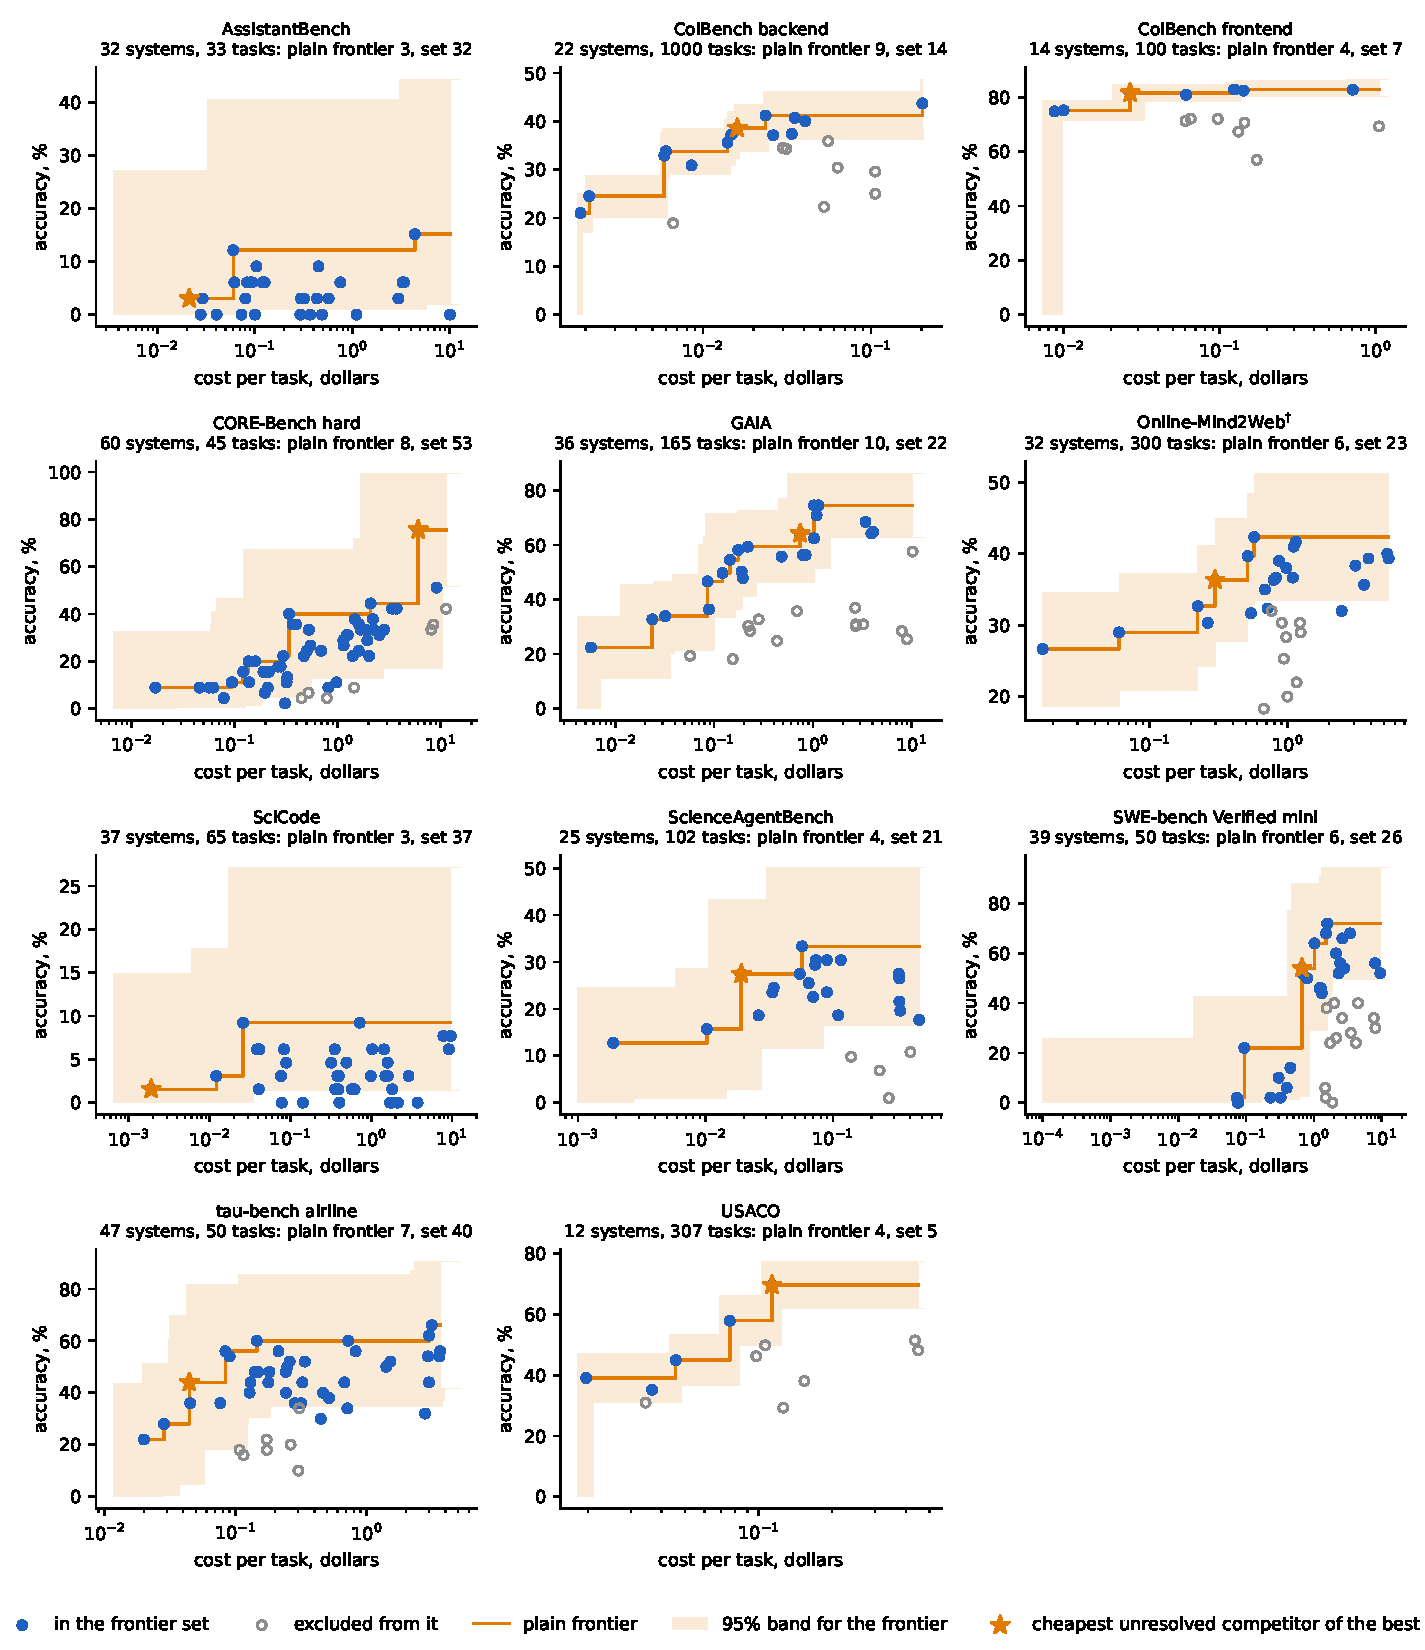
\includegraphics[width=\textwidth]{../figures/figS_all_frontiers.pdf}
\caption{Cost per task against accuracy on every HAL benchmark. The orange staircase is the observed frontier. Filled points are systems that cannot be excluded from the frontier at the 5\% level. The star is the cheapest unresolved competitor of the best. The shaded region is the 95\% simultaneous band for the frontier curve.}
\end{figure}
\begin{figure}[h]
\centering
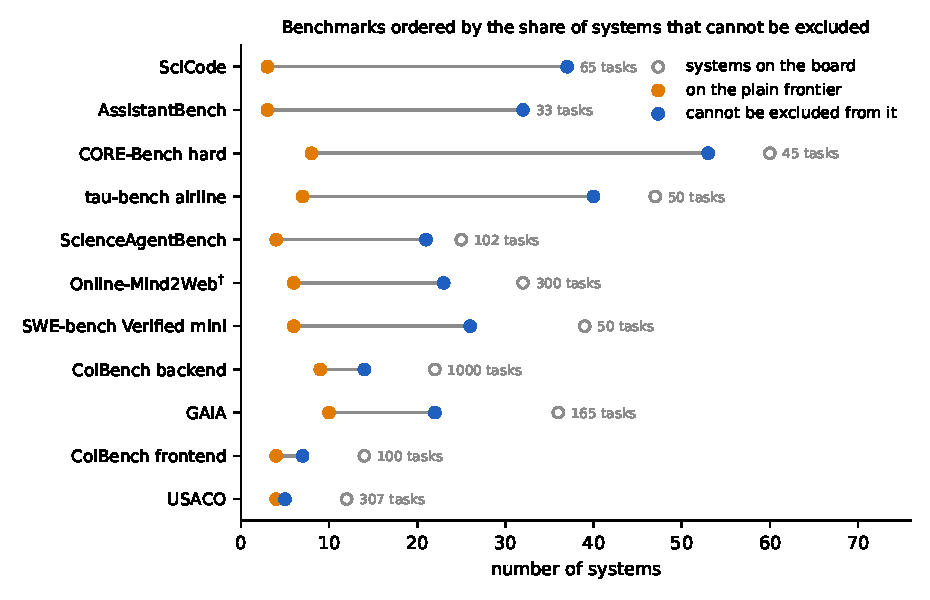
\includegraphics[width=0.75\textwidth]{../figures/fig2_setsizes.pdf}
\caption{For each benchmark, we show three counts. Orange is the number of systems on the plain frontier. Blue is the number that cannot be excluded from it at the 5\% level. Hollow is the number of systems on the board. The task count of each benchmark is shown beside it.}
\end{figure}

\begin{figure}[h]
\centering
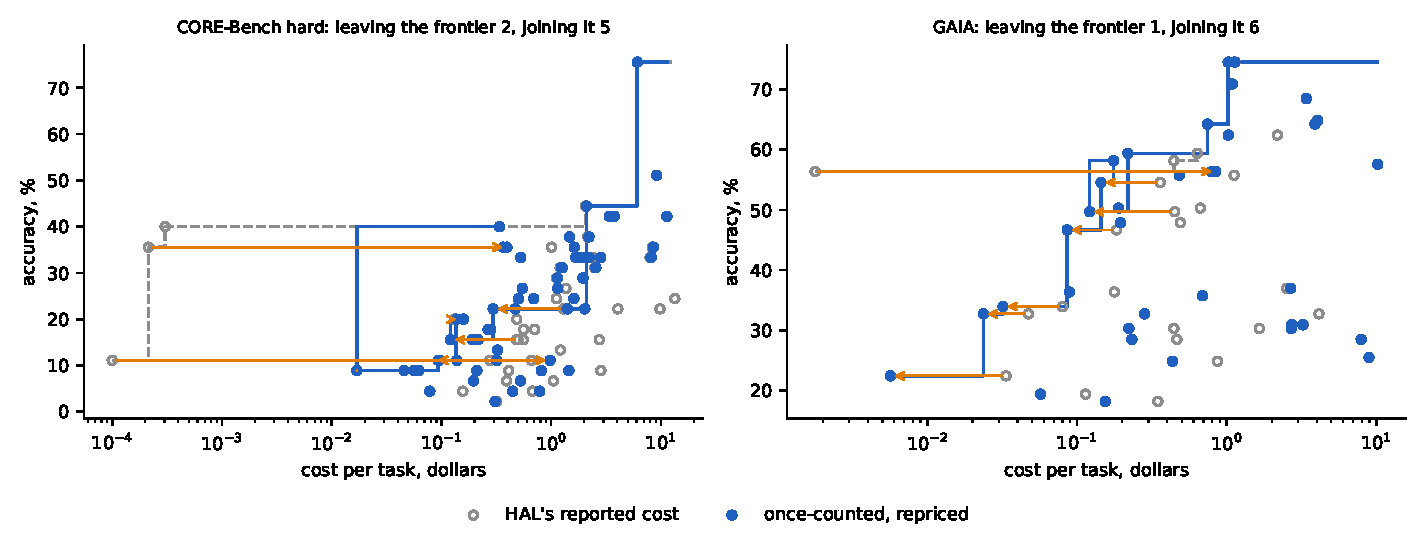
\includegraphics[width=\textwidth]{../figures/fig3_flips.pdf}
\caption{HAL's published frontier (hollow points, dashed staircase, HAL's reported costs) is shown against the frontier under once-counted, repriced costs (filled points, solid staircase), on the two boards that change most. Arrows join the two costs of each system whose frontier status changes. Costs of zero are drawn at $10^{-4}$ dollars.}
\end{figure}

\section*{S9. Every archive: HAL's total, our recount, and the run's status}
{\scriptsize\setlength{\tabcolsep}{3pt}
\begin{longtable}{llrrrl}
\caption{Every HAL archive: the benchmark, the archive's name, HAL's reported total cost, the ratio of HAL's token total to the once-counted token total, our once-counted and repriced total cost, and the run's status. The same table, with agent names and the number of duplicate calls, is in \texttt{results/hal\_reconciliation.csv}.}\label{tab:supp-reconciliation}\\
\toprule
Benchmark & Archive & Reported & Ratio & Recounted & Status \\
\midrule
\endfirsthead
\toprule
Benchmark & Archive & Reported & Ratio & Recounted & Status \\
\midrule
\endhead
\bottomrule
\endfoot
 & \texttt{\scriptsize scicode\_hal\_generalist\_agent\_gem~} &  &  &  & skipped: results member cannot~ \\
 & \texttt{\scriptsize seeact\_gpt-5\_reasoning\_effort\_hi~} &  &  &  & skipped: 12.8 GB upload cannot~ \\
 & \texttt{\scriptsize usaco\_hal\_generalist\_agent\_gpt41~} &  &  &  & skipped: results member (3.9 G~ \\
 & \texttt{\scriptsize usaco\_usaco\_episodic\_\_semantic\_c~} &  &  &  & skipped: MemberTooLarge: resul~ \\
 & \texttt{\scriptsize usaco\_usaco\_episodic\_\_semantic\_g~} &  &  &  & skipped: MemberTooLarge: resul~ \\
assistantbench & \texttt{\scriptsize assistantbench\_assistantbench\_br~} & 56.00 & 3.92 & 14.32 & kept \\
assistantbench & \texttt{\scriptsize assistantbench\_assistantbench\_br~} & 16.13 & 1.00 & 16.13 & kept \\
assistantbench & \texttt{\scriptsize assistantbench\_assistantbench\_br~} & 14.88 & 1.00 & 14.88 & kept \\
assistantbench & \texttt{\scriptsize assistantbench\_assistantbench\_br~} & 385.43 & 3.92 & 98.45 & kept \\
assistantbench & \texttt{\scriptsize assistantbench\_assistantbench\_br~} & 779.72 & 2.34 & 333.11 & kept \\
assistantbench & \texttt{\scriptsize assistantbench\_assistantbench\_br~} & 75.60 & 3.99 & 18.96 & kept \\
assistantbench & \texttt{\scriptsize assistantbench\_assistantbench\_br~} & 0.00 & 3.98 & 24.93 & kept \\
assistantbench & \texttt{\scriptsize assistantbench\_assistantbench\_br~} & 5.30 & 3.97 & 1.34 & kept \\
assistantbench & \texttt{\scriptsize assistantbench\_assistantbench\_br~} & 12.66 & 3.81 & 3.32 & kept \\
assistantbench & \texttt{\scriptsize assistantbench\_assistantbench\_br~} & 86.45 & 2.37 & 36.53 & kept \\
assistantbench & \texttt{\scriptsize assistantbench\_assistantbench\_br~} & 0.00 &  & 0.00 & dropped: no logged model calls~ \\
assistantbench & \texttt{\scriptsize assistantbench\_assistantbench\_br~} & 2.18 & 2.37 & 0.92 & kept \\
assistantbench & \texttt{\scriptsize assistantbench\_assistantbench\_br~} & 14.15 & 3.77 & 2.76 & kept \\
assistantbench & \texttt{\scriptsize assistantbench\_assistantbench\_br~} & 41.84 & 3.72 & 9.68 & kept \\
assistantbench & \texttt{\scriptsize assistantbench\_assistantbench\_br~} & 41.69 & 3.79 & 9.75 & kept \\
assistantbench & \texttt{\scriptsize assistantbench\_assistantbench\_br~} & 60.24 & 3.97 & 2.20 & dropped: outcome coverage 0.00 \\
assistantbench & \texttt{\scriptsize assistantbench\_assistantbench\_br~} & 75.77 & 3.95 & 2.93 & kept \\
assistantbench & \texttt{\scriptsize assistantbench\_assistantbench\_br~} & 12.50 & 3.70 & 3.10 & kept \\
assistantbench & \texttt{\scriptsize assistantbench\_assistantbench\_br~} & 16.39 & 3.86 & 3.95 & kept \\
assistantbench & \texttt{\scriptsize assistantbench\_assistantbench\_br~} & 9.22 & 3.93 & 2.04 & kept \\
assistantbench & \texttt{\scriptsize assistantbench\_hal\_generalist\_ag~} & 9.71 & 1.00 & 9.71 & kept \\
assistantbench & \texttt{\scriptsize assistantbench\_hal\_generalist\_ag~} & 10.56 & 1.00 & 10.56 & kept \\
assistantbench & \texttt{\scriptsize assistantbench\_hal\_generalist\_ag~} & 9.81 & 1.00 & 9.81 & kept \\
assistantbench & \texttt{\scriptsize assistantbench\_hal\_generalist\_ag~} & 108.47 & 1.00 & 108.46 & kept \\
assistantbench & \texttt{\scriptsize assistantbench\_hal\_generalist\_ag~} & 112.61 & 1.00 & 112.61 & kept \\
assistantbench & \texttt{\scriptsize assistantbench\_hal\_generalist\_ag~} & 145.01 & 1.00 & 145.01 & kept \\
assistantbench & \texttt{\scriptsize assistantbench\_hal\_generalist\_ag~} & 24.44 & 2.00 & 12.22 & kept \\
assistantbench & \texttt{\scriptsize assistantbench\_hal\_generalist\_ag~} & 3.98 & 2.00 & 1.99 & kept \\
assistantbench & \texttt{\scriptsize assistantbench\_hal\_generalist\_ag~} & 1.40 & 2.00 & 0.70 & kept \\
assistantbench & \texttt{\scriptsize assistantbench\_hal\_generalist\_ag~} & 10.83 & 2.00 & 3.43 & kept \\
assistantbench & \texttt{\scriptsize assistantbench\_hal\_generalist\_ag~} & 30.93 & 2.00 & 2.41 & kept \\
assistantbench & \texttt{\scriptsize assistantbench\_hal\_generalist\_ag~} & 5.90 & 2.00 & 2.64 & kept \\
assistantbench & \texttt{\scriptsize assistantbench\_hal\_generalist\_ag~} & 8.84 & 2.00 & 4.18 & kept \\
assistantbench & \texttt{\scriptsize assistantbench\_hal\_generalist\_ag~} & 2.11 & 2.00 & 0.96 & kept \\
colbench\_backe & \texttt{\scriptsize colbench\_backend\_programming\_col~} & 23.63 & 1.00 & 23.63 & kept \\
colbench\_backe & \texttt{\scriptsize colbench\_backend\_programming\_col~} & 40.60 & 1.00 & 40.60 & kept \\
colbench\_backe & \texttt{\scriptsize colbench\_backend\_programming\_col~} & 35.15 & 1.00 & 35.15 & kept \\
colbench\_backe & \texttt{\scriptsize colbench\_backend\_programming\_col~} & 2.10 & 1.00 & 2.10 & kept \\
colbench\_backe & \texttt{\scriptsize colbench\_backend\_programming\_col~} & 6.01 & 1.00 & 6.01 & kept \\
colbench\_backe & \texttt{\scriptsize colbench\_backend\_programming\_col~} & 52.55 & 1.00 & 52.55 & kept \\
colbench\_backe & \texttt{\scriptsize colbench\_backend\_programming\_col~} & 106.60 & 1.00 & 26.19 & kept \\
colbench\_backe & \texttt{\scriptsize colbench\_backend\_programming\_col~} & 31.38 & 1.00 & 31.38 & kept \\
colbench\_backe & \texttt{\scriptsize colbench\_backend\_programming\_col~} & 14.73 & 1.00 & 14.72 & kept \\
colbench\_backe & \texttt{\scriptsize colbench\_backend\_programming\_col~} & 204.80 & 1.92 & 105.94 & kept \\
colbench\_backe & \texttt{\scriptsize colbench\_backend\_programming\_col~} & 53.26 & 1.89 & 29.85 & kept \\
colbench\_backe & \texttt{\scriptsize colbench\_backend\_programming\_col~} & 15.99 & 1.00 & 15.99 & kept \\
colbench\_backe & \texttt{\scriptsize colbench\_backend\_programming\_col~} & 143.33 & 1.89 & 55.63 & kept \\
colbench\_backe & \texttt{\scriptsize colbench\_backend\_programming\_col~} & 1,299.27 & 1.96 & 106.11 & kept \\
colbench\_backe & \texttt{\scriptsize colbench\_backend\_programming\_col~} & 138.13 & 1.92 & 63.29 & kept \\
colbench\_backe & \texttt{\scriptsize colbench\_backend\_programming\_col~} & 4.14 & 1.00 & 4.14 & kept \\
colbench\_backe & \texttt{\scriptsize colbench\_backend\_programming\_col~} & 1.49 & 1.00 & 1.49 & kept \\
colbench\_backe & \texttt{\scriptsize colbench\_backend\_programming\_col~} & 5.88 & 1.00 & 5.88 & kept \\
colbench\_backe & \texttt{\scriptsize colbench\_backend\_programming\_col~} & 13.99 & 1.00 & 13.99 & kept \\
colbench\_backe & \texttt{\scriptsize colbench\_backend\_programming\_col~} & 8.55 & 1.00 & 8.55 & kept \\
colbench\_backe & \texttt{\scriptsize colbench\_backend\_programming\_col~} & 33.77 & 1.00 & 33.77 & kept \\
colbench\_backe & \texttt{\scriptsize colbench\_backend\_programming\_hal~} & 202.35 & 1.00 & 202.35 & kept \\
colbench\_front & \texttt{\scriptsize colbench\_frontend\_design\_colbenc~} & 33.28 & 1.92 & 17.24 & kept \\
colbench\_front & \texttt{\scriptsize colbench\_frontend\_design\_colbenc~} & 11.08 & 1.93 & 6.03 & kept \\
colbench\_front & \texttt{\scriptsize colbench\_frontend\_design\_colbenc~} & 15.71 & 1.91 & 6.52 & kept \\
colbench\_front & \texttt{\scriptsize colbench\_frontend\_design\_colbenc~} & 20.62 & 1.92 & 9.70 & kept \\
colbench\_front & \texttt{\scriptsize colbench\_frontend\_design\_colbenc~} & 153.99 & 1.95 & 13.16 & kept \\
colbench\_front & \texttt{\scriptsize colbench\_frontend\_design\_colbenc~} & 29.43 & 1.90 & 14.41 & kept \\
colbench\_front & \texttt{\scriptsize colbench\_frontend\_design\_colbenc~} & 0.85 & 1.00 & 0.85 & kept \\
colbench\_front & \texttt{\scriptsize colbench\_frontend\_design\_colbenc~} & 0.84 & 1.00 & 0.84 & kept \\
colbench\_front & \texttt{\scriptsize colbench\_frontend\_design\_colbenc~} & 2.66 & 1.00 & 2.66 & kept \\
colbench\_front & \texttt{\scriptsize colbench\_frontend\_design\_colbenc~} & 14.57 & 1.00 & 14.23 & kept \\
colbench\_front & \texttt{\scriptsize colbench\_frontend\_design\_colbenc~} & 6.21 & 1.00 & 6.08 & kept \\
colbench\_front & \texttt{\scriptsize colbench\_frontend\_design\_colbenc~} & 12.76 & 1.00 & 12.35 & kept \\
colbench\_front & \texttt{\scriptsize colbench\_frontend\_design\_colbenc~} & 71.30 & 1.00 & 71.30 & kept \\
colbench\_front & \texttt{\scriptsize colbench\_frontend\_design\_halgene~} & 104.84 & 1.00 & 104.84 & kept \\
corebench\_hard & \texttt{\scriptsize corebench\_hard\_claude\_code\_claud~} & 331.79 &  & 0.00 & dropped: no logged model calls~ \\
corebench\_hard & \texttt{\scriptsize corebench\_hard\_claude\_code\_claud~} & 87.16 &  & 0.00 & dropped: no logged model calls~ \\
corebench\_hard & \texttt{\scriptsize corebench\_hard\_claude\_code\_claud~} & 65.58 &  & 0.00 & dropped: no logged model calls~ \\
corebench\_hard & \texttt{\scriptsize corebench\_hard\_claude\_code\_claud~} & 68.33 &  & 0.00 & dropped: no logged model calls~ \\
corebench\_hard & \texttt{\scriptsize corebench\_hard\_core\_agent\_176384~} & 0.01 & 2.00 & 15.22 & kept \\
corebench\_hard & \texttt{\scriptsize corebench\_hard\_core\_agent\_opus\_4~} & 168.99 & 1.00 & 168.97 & kept \\
corebench\_hard & \texttt{\scriptsize corebench\_hard\_core\_agent\_opus\_4~} & 152.66 & 1.00 & 152.56 & kept \\
corebench\_hard & \texttt{\scriptsize corebench\_hard\_coreagent\_1744752~} & 107.36 & 2.00 & 23.73 & kept \\
corebench\_hard & \texttt{\scriptsize corebench\_hard\_coreagent\_1744839~} & 21.86 & 2.00 & 7.15 & kept \\
corebench\_hard & \texttt{\scriptsize corebench\_hard\_coreagent\_1744854~} & 25.26 & 2.00 & 12.63 & kept \\
corebench\_hard & \texttt{\scriptsize corebench\_hard\_coreagent\_1744856~} & 12.46 & 2.00 & 6.23 & kept \\
corebench\_hard & \texttt{\scriptsize corebench\_hard\_coreagent\_1744922~} & 73.04 & 1.00 & 72.99 & kept \\
corebench\_hard & \texttt{\scriptsize corebench\_hard\_coreagent\_1744922~} & 182.34 & 2.00 & 91.17 & kept \\
corebench\_hard & \texttt{\scriptsize corebench\_hard\_coreagent\_1744922~} & 25.06 & 2.00 & 8.63 & kept \\
corebench\_hard & \texttt{\scriptsize corebench\_hard\_coreagent\_1744922~} & 127.57 & 2.00 & 63.78 & kept \\
corebench\_hard & \texttt{\scriptsize corebench\_hard\_coreagent\_1745046~} & 31.79 & 2.00 & 12.00 & kept \\
corebench\_hard & \texttt{\scriptsize corebench\_hard\_coreagent\_1745075~} & 61.35 & 2.00 & 24.57 & kept \\
corebench\_hard & \texttt{\scriptsize corebench\_hard\_coreagent\_1745118~} & 602.37 & 2.00 & 31.16 & kept \\
corebench\_hard & \texttt{\scriptsize corebench\_hard\_coreagent\_1745118~} & 75.19 & 1.00 & 75.19 & kept \\
corebench\_hard & \texttt{\scriptsize corebench\_hard\_coreagent\_1745258~} & 72.47 & 1.00 & 72.40 & kept \\
corebench\_hard & \texttt{\scriptsize corebench\_hard\_coreagent\_1754492~} & 4.21 & 1.00 & 4.21 & kept \\
corebench\_hard & \texttt{\scriptsize corebench\_hard\_coreagent\_1754492~} & 412.42 & 1.00 & 412.40 & kept \\
corebench\_hard & \texttt{\scriptsize corebench\_hard\_coreagent\_1754539~} & 4.21 & 1.00 & 4.20 & kept \\
corebench\_hard & \texttt{\scriptsize corebench\_hard\_coreagent\_1754539~} & 509.95 & 1.00 & 509.89 & kept \\
corebench\_hard & \texttt{\scriptsize corebench\_hard\_coreagent\_1754599~} & 31.76 &  & 0.00 & dropped: no logged model calls~ \\
corebench\_hard & \texttt{\scriptsize corebench\_hard\_coreagentclaudeha~} & 0.00 & 1.00 & 43.93 & kept \\
corebench\_hard & \texttt{\scriptsize corebench\_hard\_coreagentclaudeop~} & 273.74 & 1.00 & 273.69 & kept \\
corebench\_hard & \texttt{\scriptsize corebench\_hard\_coreagentclaudeso~} & 97.15 & 1.00 & 97.14 & kept \\
corebench\_hard & \texttt{\scriptsize corebench\_hard\_coreagentclaudeso~} & 92.34 & 1.00 & 92.33 & kept \\
corebench\_hard & \texttt{\scriptsize corebench\_hard\_coreagentclaudeso~} & 50.27 & 1.00 & 50.18 & kept \\
corebench\_hard & \texttt{\scriptsize corebench\_hard\_coreagentclaudeso~} & 100.48 & 1.00 & 100.42 & kept \\
corebench\_hard & \texttt{\scriptsize corebench\_hard\_coreagentdeepseek~} & 35.43 & 1.00 & 34.66 & kept \\
corebench\_hard & \texttt{\scriptsize corebench\_hard\_coreagentdeepseek~} & 5.91 & 1.00 & 5.87 & kept \\
corebench\_hard & \texttt{\scriptsize corebench\_hard\_hal\_generalist\_ag~} & 54.61 & 2.00 & 13.99 & kept \\
corebench\_hard & \texttt{\scriptsize corebench\_hard\_hal\_generalist\_ag~} & 18.50 & 2.00 & 9.25 & kept \\
corebench\_hard & \texttt{\scriptsize corebench\_hard\_hal\_generalist\_ag~} & 0.16 & 1.00 & 0.16 & dropped: no logged model calls~ \\
corebench\_hard & \texttt{\scriptsize corebench\_hard\_hal\_generalist\_ag~} & 17.68 & 2.00 & 8.84 & kept \\
corebench\_hard & \texttt{\scriptsize corebench\_hard\_hal\_generalist\_ag~} & 21.80 & 2.00 & 9.38 & kept \\
corebench\_hard & \texttt{\scriptsize corebench\_hard\_hal\_generalist\_ag~} & 47.10 & 2.00 & 23.55 & kept \\
corebench\_hard & \texttt{\scriptsize corebench\_hard\_hal\_generalist\_ag~} & 30.38 & 2.00 & 15.19 & kept \\
corebench\_hard & \texttt{\scriptsize corebench\_hard\_hal\_generalist\_ag~} & 50.28 & 2.00 & 22.69 & kept \\
corebench\_hard & \texttt{\scriptsize corebench\_hard\_hal\_generalist\_ag~} & 123.50 & 2.00 & 8.57 & kept \\
corebench\_hard & \texttt{\scriptsize corebench\_hard\_hal\_generalist\_ag~} & 36.67 & 1.00 & 36.67 & kept \\
corebench\_hard & \texttt{\scriptsize corebench\_hard\_hal\_generalist\_ag~} & 63.21 & 1.00 & 63.21 & kept \\
corebench\_hard & \texttt{\scriptsize corebench\_hard\_hal\_generalist\_ag~} & 51.59 & 1.00 & 51.59 & kept \\
corebench\_hard & \texttt{\scriptsize corebench\_hard\_hal\_generalist\_ag~} & 54.37 & 1.00 & 54.37 & kept \\
corebench\_hard & \texttt{\scriptsize corebench\_hard\_hal\_generalist\_ag~} & 2.79 & 1.00 & 2.79 & kept \\
corebench\_hard & \texttt{\scriptsize corebench\_hard\_hal\_generalist\_ag~} & 375.11 & 1.00 & 375.11 & kept \\
corebench\_hard & \texttt{\scriptsize corebench\_hard\_hal\_generalist\_ag~} & 2.05 & 1.00 & 2.05 & kept \\
corebench\_hard & \texttt{\scriptsize corebench\_hard\_hal\_generalist\_ag~} & 358.47 & 1.00 & 358.47 & kept \\
corebench\_hard & \texttt{\scriptsize corebench\_hard\_hal\_generalist\_ag~} & 0.01 & 2.00 & 17.38 & kept \\
corebench\_hard & \texttt{\scriptsize corebench\_hard\_hal\_generalist\_ag~} & 127.41 & 1.00 & 127.40 & kept \\
corebench\_hard & \texttt{\scriptsize corebench\_hard\_hal\_generalist\_ag~} & 112.38 & 1.00 & 112.37 & kept \\
corebench\_hard & \texttt{\scriptsize corebench\_hard\_hal\_generalist\_ag~} & 2.55 & 1.00 & 2.55 & kept \\
corebench\_hard & \texttt{\scriptsize corebench\_hard\_hal\_generalist\_ag~} & 14.37 & 1.00 & 13.87 & kept \\
corebench\_hard & \texttt{\scriptsize corebench\_hard\_hal\_generalist\_ag~} & 0.76 & 1.00 & 0.76 & kept \\
corebench\_hard & \texttt{\scriptsize corebench\_hard\_hal\_generalist\_ag~} & 7.06 & 2.00 & 3.53 & kept \\
corebench\_hard & \texttt{\scriptsize corebench\_hard\_hal\_generalist\_ag~} & 58.32 & 2.00 & 13.32 & kept \\
corebench\_hard & \texttt{\scriptsize corebench\_hard\_hal\_generalist\_ag~} & 29.75 & 2.00 & 14.07 & kept \\
corebench\_hard & \texttt{\scriptsize corebench\_hard\_hal\_generalist\_ag~} & 441.70 & 2.00 & 20.68 & kept \\
corebench\_hard & \texttt{\scriptsize corebench\_hard\_hal\_generalist\_ag~} & 45.37 & 2.00 & 16.44 & kept \\
corebench\_hard & \texttt{\scriptsize corebench\_hard\_hal\_generalist\_ag~} & 22.50 & 2.00 & 5.45 & kept \\
corebench\_hard & \texttt{\scriptsize corebench\_hard\_hal\_generalist\_ag~} & 56.64 & 1.00 & 56.62 & kept \\
corebench\_hard & \texttt{\scriptsize corebench\_hard\_hal\_generalist\_ag~} & 66.15 & 1.00 & 66.11 & kept \\
corebench\_hard & \texttt{\scriptsize corebench\_hard\_halgeneralistagen~} & 85.19 & 1.00 & 85.13 & kept \\
corebench\_hard & \texttt{\scriptsize corebench\_hard\_halgeneralistagen~} & 87.77 & 1.00 & 87.75 & kept \\
gaia & \texttt{\scriptsize gaia\_hal\_generalist\_agent\_claude~} & 130.68 & 1.00 & 130.52 & kept \\
gaia & \texttt{\scriptsize gaia\_hal\_generalist\_agent\_claude~} & 122.49 & 1.00 & 122.39 & kept \\
gaia & \texttt{\scriptsize gaia\_hal\_generalist\_agent\_claude~} & 0.29 & 1.00 & 130.66 & kept \\
gaia & \texttt{\scriptsize gaia\_hal\_generalist\_agent\_claude~} & 562.24 & 1.00 & 562.14 & kept \\
gaia & \texttt{\scriptsize gaia\_hal\_generalist\_agent\_claude~} & 641.86 & 1.00 & 641.73 & kept \\
gaia & \texttt{\scriptsize gaia\_hal\_generalist\_agent\_claude~} & 272.76 & 1.00 & 272.73 & kept \\
gaia & \texttt{\scriptsize gaia\_hal\_generalist\_agent\_claude~} & 665.89 & 1.00 & 665.75 & kept \\
gaia & \texttt{\scriptsize gaia\_hal\_generalist\_agent\_claude~} & 179.86 & 1.00 & 179.61 & kept \\
gaia & \texttt{\scriptsize gaia\_hal\_generalist\_agent\_claude~} & 187.37 & 1.00 & 187.06 & kept \\
gaia & \texttt{\scriptsize gaia\_hal\_generalist\_agent\_claude~} & 169.02 & 1.00 & 168.83 & kept \\
gaia & \texttt{\scriptsize gaia\_hal\_generalist\_agent\_deepse~} & 73.19 & 2.00 & 36.60 & kept \\
gaia & \texttt{\scriptsize gaia\_hal\_generalist\_agent\_deepse~} & 29.27 & 2.00 & 14.63 & kept \\
gaia & \texttt{\scriptsize gaia\_hal\_generalist\_agent\_deepse~} & 5.52 & 1.00 & 0.93 & kept \\
gaia & \texttt{\scriptsize gaia\_hal\_generalist\_agent\_gemini~} & 7.80 & 2.00 & 3.90 & kept \\
gaia & \texttt{\scriptsize gaia\_hal\_generalist\_agent\_gpt412~} & 74.19 & 2.00 & 20.03 & kept \\
gaia & \texttt{\scriptsize gaia\_hal\_generalist\_agent\_gpt520~} & 104.75 & 2.00 & 36.11 & kept \\
gaia & \texttt{\scriptsize gaia\_hal\_generalist\_agent\_o32025~} & 2,828.54 &  & 0.00 & dropped: no logged model calls~ \\
gaia & \texttt{\scriptsize gaia\_hal\_generalist\_agent\_o3mini~} & 13.19 & 2.00 & 5.28 & kept \\
gaia & \texttt{\scriptsize gaia\_hal\_generalist\_agent\_o3mini~} & 30.37 & 2.00 & 14.18 & kept \\
gaia & \texttt{\scriptsize gaia\_hal\_generalist\_agent\_o4mini~} & 59.39 & 2.00 & 23.85 & kept \\
gaia & \texttt{\scriptsize gaia\_hal\_generalist\_agent\_o4mini~} & 73.26 & 2.00 & 28.94 & kept \\
gaia & \texttt{\scriptsize gaia\_hf\_open\_deep\_research\_claud~} & 415.15 & 1.00 & 415.15 & kept \\
gaia & \texttt{\scriptsize gaia\_hf\_open\_deep\_research\_claud~} & 113.65 & 1.00 & 113.65 & kept \\
gaia & \texttt{\scriptsize gaia\_hf\_open\_deep\_research\_claud~} & 1,306.85 & 1.00 & 1,306.85 & kept \\
gaia & \texttt{\scriptsize gaia\_hf\_open\_deep\_research\_claud~} & 1,473.64 & 1.00 & 1,473.64 & kept \\
gaia & \texttt{\scriptsize gaia\_hf\_open\_deep\_research\_claud~} & 1,686.07 & 1.00 & 1,686.07 & kept \\
gaia & \texttt{\scriptsize gaia\_hf\_open\_deep\_research\_claud~} & 535.00 & 1.01 & 532.54 & kept \\
gaia & \texttt{\scriptsize gaia\_hf\_open\_deep\_research\_claud~} & 451.84 & 1.01 & 449.42 & kept \\
gaia & \texttt{\scriptsize gaia\_hf\_open\_deep\_research\_deeps~} & 143.08 & 2.00 & 71.54 & kept \\
gaia & \texttt{\scriptsize gaia\_hf\_open\_deep\_research\_deeps~} & 76.64 & 2.00 & 38.32 & kept \\
gaia & \texttt{\scriptsize gaia\_hf\_open\_deep\_research\_gemin~} & 18.82 & 2.00 & 9.41 & kept \\
gaia & \texttt{\scriptsize gaia\_hf\_open\_deep\_research\_gpt41~} & 109.88 & 2.00 & 31.13 & kept \\
gaia & \texttt{\scriptsize gaia\_hf\_open\_deep\_research\_gpt52~} & 359.83 & 2.00 & 168.92 & kept \\
gaia & \texttt{\scriptsize gaia\_hf\_open\_deep\_research\_o3202~} & 681.97 & 2.00 & 46.66 & kept \\
gaia & \texttt{\scriptsize gaia\_hf\_open\_deep\_research\_o3min~} & 57.24 & 2.00 & 25.31 & kept \\
gaia & \texttt{\scriptsize gaia\_hf\_open\_deep\_research\_o4min~} & 184.87 & 2.00 & 79.56 & kept \\
gaia & \texttt{\scriptsize gaia\_hf\_open\_deep\_research\_o4min~} & 80.80 & 2.00 & 32.03 & kept \\
online\_mind2we & \texttt{\scriptsize browser-use\_DeepSeek-R1} & 280.93 &  & 0.00 & kept \\
online\_mind2we & \texttt{\scriptsize browser-use\_DeepSeek-V3} & 214.74 &  & 0.00 & kept \\
online\_mind2we & \texttt{\scriptsize browser-use\_claude-3-7-sonnet-20~} & 926.48 &  & 0.00 & kept \\
online\_mind2we & \texttt{\scriptsize browser-use\_claude-3-7-sonnet-20~} & 1,151.88 &  & 0.00 & kept \\
online\_mind2we & \texttt{\scriptsize browser-use\_claude-haiku-4-5-202~} & 598.68 &  & 0.00 & dropped: outcome coverage 0.88 \\
online\_mind2we & \texttt{\scriptsize browser-use\_claude-haiku-4-5-202~} & 617.52 &  & 0.00 & dropped: outcome coverage 0.88 \\
online\_mind2we & \texttt{\scriptsize browser-use\_claude-sonnet-4-2025~} & 1,577.26 &  & 0.00 & kept \\
online\_mind2we & \texttt{\scriptsize browser-use\_claude-sonnet-4-2025~} & 1,609.92 &  & 0.00 & kept \\
online\_mind2we & \texttt{\scriptsize browser-use\_claude-sonnet-4-5-20~} & 1,659.81 &  & 0.00 & dropped: outcome coverage 0.88 \\
online\_mind2we & \texttt{\scriptsize browser-use\_claude-sonnet-4-5-20~} & 1,669.28 &  & 0.00 & dropped: outcome coverage 0.88 \\
online\_mind2we & \texttt{\scriptsize browser-use\_gemini-2.0-flash} & 18.01 &  & 0.00 & kept \\
online\_mind2we & \texttt{\scriptsize browser-use\_gemini-2.5-pro-previ~} & 331.37 &  & 0.00 & kept \\
online\_mind2we & \texttt{\scriptsize browser-use\_gpt-4.1-2025-04-14} & 236.62 &  & 0.00 & kept \\
online\_mind2we & \texttt{\scriptsize browser-use\_gpt-5\_reasoning\_effo~} & 1,069.59 &  & 0.00 & kept \\
online\_mind2we & \texttt{\scriptsize browser-use\_gpt-5\_reasoning\_effo~} & 736.31 &  & 0.00 & kept \\
online\_mind2we & \texttt{\scriptsize browser-use\_gpt-5\_reasoning\_effo~} & 347.23 &  & 0.00 & kept \\
online\_mind2we & \texttt{\scriptsize browser-use\_o3-2025-04-16} & 1,857.94 &  & 0.00 & kept \\
online\_mind2we & \texttt{\scriptsize browser-use\_o4-mini\_reasoning\_ef~} & 297.93 &  & 0.00 & kept \\
online\_mind2we & \texttt{\scriptsize browser-use\_o4-mini\_reasoning\_ef~} & 201.44 &  & 0.00 & kept \\
online\_mind2we & \texttt{\scriptsize seeact\_claude-3-7-sonnet-20250219} & 291.97 &  & 0.00 & kept \\
online\_mind2we & \texttt{\scriptsize seeact\_claude-3-7-sonnet-2025021~} & 367.51 &  & 0.00 & kept \\
online\_mind2we & \texttt{\scriptsize seeact\_claude-haiku-4-5-20251001} & 66.78 &  & 0.00 & kept \\
online\_mind2we & \texttt{\scriptsize seeact\_claude-haiku-4-5-20251001~} & 89.17 &  & 0.00 & kept \\
online\_mind2we & \texttt{\scriptsize seeact\_claude-sonnet-4-20250514} & 246.18 &  & 0.00 & kept \\
online\_mind2we & \texttt{\scriptsize seeact\_claude-sonnet-4-20250514\_~} & 326.41 &  & 0.00 & kept \\
online\_mind2we & \texttt{\scriptsize seeact\_claude-sonnet-4-5-20250929} & 204.86 &  & 0.00 & kept \\
online\_mind2we & \texttt{\scriptsize seeact\_claude-sonnet-4-5-2025092~} & 293.15 &  & 0.00 & kept \\
online\_mind2we & \texttt{\scriptsize seeact\_gemini-2.0-flash} & 5.03 &  & 0.00 & kept \\
online\_mind2we & \texttt{\scriptsize seeact\_gemini-2.5-pro-preview-03~} & 153.61 &  & 0.00 & kept \\
online\_mind2we & \texttt{\scriptsize seeact\_gpt-4.1-2025-04-14} & 271.24 &  & 0.00 & kept \\
online\_mind2we & \texttt{\scriptsize seeact\_gpt-5\_reasoning\_effort\_hi~} & 342.93 &  & 0.00 & kept \\
online\_mind2we & \texttt{\scriptsize seeact\_gpt-5\_reasoning\_effort\_me~} & 171.07 &  & 0.00 & kept \\
online\_mind2we & \texttt{\scriptsize seeact\_gpt-5\_reasoning\_effort\_mi~} & 78.86 &  & 0.00 & kept \\
online\_mind2we & \texttt{\scriptsize seeact\_o3-2025-04-16} & 1,293.69 &  & 0.00 & kept \\
online\_mind2we & \texttt{\scriptsize seeact\_o4-mini\_reasoning\_effort\_~} & 228.98 &  & 0.00 & kept \\
online\_mind2we & \texttt{\scriptsize seeact\_o4-mini\_reasoning\_effort\_~} & 162.36 &  & 0.00 & kept \\
scicode & \texttt{\scriptsize scicode\_hal\_generalist\_agent\_cla~} & 60.40 & 1.00 & 60.40 & kept \\
scicode & \texttt{\scriptsize scicode\_hal\_generalist\_agent\_cla~} & 188.15 & 1.00 & 188.15 & kept \\
scicode & \texttt{\scriptsize scicode\_hal\_generalist\_agent\_dee~} & 486.78 & 2.00 & 243.39 & kept \\
scicode & \texttt{\scriptsize scicode\_hal\_generalist\_agent\_dee~} & 219.36 & 2.00 & 109.68 & kept \\
scicode & \texttt{\scriptsize scicode\_hal\_generalist\_agent\_gpt~} & 73.87 & 2.00 & 23.32 & kept \\
scicode & \texttt{\scriptsize scicode\_hal\_generalist\_agent\_o32~} & 291.50 & 2.00 & 23.06 & kept \\
scicode & \texttt{\scriptsize scicode\_hal\_generalist\_agent\_o32~} & 334.88 & 2.00 & 24.83 & kept \\
scicode & \texttt{\scriptsize scicode\_hal\_generalist\_agent\_o4m~} & 87.69 & 2.00 & 37.47 & kept \\
scicode & \texttt{\scriptsize scicode\_hal\_generalist\_agent\_o4m~} & 92.10 & 2.00 & 39.89 & kept \\
scicode & \texttt{\scriptsize scicode\_hal\_generalist\_agent\_o4m~} & 165.90 & 2.00 & 66.87 & kept \\
scicode & \texttt{\scriptsize scicode\_scicode-tool\_calling\_age~} & 507.73 & 1.00 & 507.73 & kept \\
scicode & \texttt{\scriptsize scicode\_scicode\_tool\_calling\_age~} & 191.41 & 1.98 & 97.46 & kept \\
scicode & \texttt{\scriptsize scicode\_scicode\_tool\_calling\_age~} & 204.37 & 1.98 & 103.96 & kept \\
scicode & \texttt{\scriptsize scicode\_scicode\_tool\_calling\_age~} & 232.36 & 1.99 & 117.48 & kept \\
scicode & \texttt{\scriptsize scicode\_scicode\_tool\_calling\_age~} & 625.13 & 1.00 & 625.13 & kept \\
scicode & \texttt{\scriptsize scicode\_scicode\_tool\_calling\_age~} & 593.35 & 1.00 & 593.35 & kept \\
scicode & \texttt{\scriptsize scicode\_scicode\_tool\_calling\_age~} & 104.29 & 1.00 & 104.29 & kept \\
scicode & \texttt{\scriptsize scicode\_scicode\_tool\_calling\_age~} & 0.00 & 1.00 & 118.14 & kept \\
scicode & \texttt{\scriptsize scicode\_scicode\_tool\_calling\_age~} & 52.11 & 1.98 & 26.29 & kept \\
scicode & \texttt{\scriptsize scicode\_scicode\_tool\_calling\_age~} & 273.98 & 1.98 & 139.21 & kept \\
scicode & \texttt{\scriptsize scicode\_scicode\_tool\_calling\_age~} & 5.23 & 1.98 & 2.65 & kept \\
scicode & \texttt{\scriptsize scicode\_scicode\_tool\_calling\_age~} & 69.39 & 1.99 & 25.59 & kept \\
scicode & \texttt{\scriptsize scicode\_scicode\_tool\_calling\_age~} & 193.52 & 2.00 & 93.70 & kept \\
scicode & \texttt{\scriptsize scicode\_scicode\_tool\_calling\_age~} & 555.57 & 1.97 & 46.93 & kept \\
scicode & \texttt{\scriptsize scicode\_scicode\_tool\_calling\_age~} & 55.86 & 1.97 & 25.91 & kept \\
scicode & \texttt{\scriptsize scicode\_scicode\_tool\_calling\_age~} & 66.20 & 1.97 & 32.14 & kept \\
scicode & \texttt{\scriptsize scicode\_scicode\_tool\_calling\_age~} & 46.30 & 1.98 & 20.83 & kept \\
scicode & \texttt{\scriptsize scicode\_scicode\_zero\_shot\_agent\_~} & 5.10 & 1.00 & 5.10 & kept \\
scicode & \texttt{\scriptsize scicode\_scicode\_zero\_shot\_agent\_~} & 4.99 & 1.00 & 4.99 & kept \\
scicode & \texttt{\scriptsize scicode\_scicode\_zero\_shot\_agent\_~} & 9.18 & 1.00 & 9.18 & kept \\
scicode & \texttt{\scriptsize scicode\_scicode\_zero\_shot\_agent\_~} & 0.79 & 1.00 & 0.79 & kept \\
scicode & \texttt{\scriptsize scicode\_scicode\_zero\_shot\_agent\_~} & 0.12 & 1.00 & 0.12 & kept \\
scicode & \texttt{\scriptsize scicode\_scicode\_zero\_shot\_agent\_~} & 2.82 & 1.00 & 2.52 & kept \\
scicode & \texttt{\scriptsize scicode\_scicode\_zero\_shot\_agent\_~} & 30.16 & 1.00 & 5.79 & kept \\
scicode & \texttt{\scriptsize scicode\_scicode\_zero\_shot\_agent\_~} & 2.72 & 1.00 & 2.70 & kept \\
scicode & \texttt{\scriptsize scicode\_scicode\_zero\_shot\_agent\_~} & 5.37 & 1.00 & 5.34 & kept \\
scicode & \texttt{\scriptsize scicode\_scicode\_zero\_shot\_agent\_~} & 1.74 & 1.00 & 1.70 & kept \\
scienceagentbe & \texttt{\scriptsize scienceagentbench\_hal\_generalist~} & 41.22 & 1.00 & 41.22 & kept \\
scienceagentbe & \texttt{\scriptsize scienceagentbench\_hal\_generalist~} & 48.28 & 1.00 & 48.28 & kept \\
scienceagentbe & \texttt{\scriptsize scienceagentbench\_hal\_generalist~} & 55.73 & 2.00 & 27.87 & kept \\
scienceagentbe & \texttt{\scriptsize scienceagentbench\_hal\_generalist~} & 68.95 & 2.00 & 23.63 & kept \\
scienceagentbe & \texttt{\scriptsize scienceagentbench\_hal\_generalist~} & 155.42 & 2.00 & 14.12 & kept \\
scienceagentbe & \texttt{\scriptsize scienceagentbench\_hal\_generalist~} & 76.30 & 2.00 & 33.80 & kept \\
scienceagentbe & \texttt{\scriptsize scienceagentbench\_hal\_generalist~} & 77.32 & 2.00 & 34.32 & kept \\
scienceagentbe & \texttt{\scriptsize scienceagentbench\_sab\_selfdebug\_~} & 7.12 & 1.00 & 7.12 & kept \\
scienceagentbe & \texttt{\scriptsize scienceagentbench\_sab\_selfdebug\_~} & 11.74 & 1.00 & 11.74 & kept \\
scienceagentbe & \texttt{\scriptsize scienceagentbench\_sab\_selfdebug\_~} & 6.56 & 1.00 & 6.56 & kept \\
scienceagentbe & \texttt{\scriptsize scienceagentbench\_sab\_selfdebug\_~} & 2.66 & 1.00 & 2.66 & kept \\
scienceagentbe & \texttt{\scriptsize scienceagentbench\_sab\_selfdebug\_~} & 3.41 & 1.00 & 3.41 & kept \\
scienceagentbe & \texttt{\scriptsize scienceagentbench\_sab\_selfdebug\_~} & 33.37 & 1.00 & 33.37 & kept \\
scienceagentbe & \texttt{\scriptsize scienceagentbench\_sab\_selfdebug\_~} & 33.75 & 1.00 & 33.75 & kept \\
scienceagentbe & \texttt{\scriptsize scienceagentbench\_sab\_selfdebug\_~} & 7.39 & 1.00 & 7.39 & kept \\
scienceagentbe & \texttt{\scriptsize scienceagentbench\_sab\_selfdebug\_~} & 7.47 & 1.00 & 7.47 & kept \\
scienceagentbe & \texttt{\scriptsize scienceagentbench\_sab\_selfdebug\_~} & 18.24 & 2.00 & 9.12 & kept \\
scienceagentbe & \texttt{\scriptsize scienceagentbench\_sab\_selfdebug\_~} & 2.09 & 2.00 & 1.05 & kept \\
scienceagentbe & \texttt{\scriptsize scienceagentbench\_sab\_selfdebug\_~} & 0.19 & 1.00 & 0.19 & kept \\
scienceagentbe & \texttt{\scriptsize scienceagentbench\_sab\_selfdebug\_~} & 11.20 & 1.00 & 11.20 & kept \\
scienceagentbe & \texttt{\scriptsize scienceagentbench\_sab\_selfdebug\_~} & 18.26 & 2.00 & 9.12 & kept \\
scienceagentbe & \texttt{\scriptsize scienceagentbench\_sab\_selfdebug\_~} & 7.42 & 2.00 & 3.49 & kept \\
scienceagentbe & \texttt{\scriptsize scienceagentbench\_sab\_selfdebug\_~} & 58.44 & 2.00 & 5.83 & kept \\
scienceagentbe & \texttt{\scriptsize scienceagentbench\_sab\_selfdebug\_~} & 11.18 & 2.00 & 5.59 & kept \\
scienceagentbe & \texttt{\scriptsize scienceagentbench\_sab\_selfdebug\_~} & 3.95 & 2.00 & 1.94 & kept \\
swebench\_verif & \texttt{\scriptsize swebench\_verified\_mini\_1743738168} & 350.72 & 2.00 & 175.36 & kept \\
swebench\_verif & \texttt{\scriptsize swebench\_verified\_mini\_1743879454} & 113.33 & 2.00 & 33.31 & dropped: outcome coverage 0.92 \\
swebench\_verif & \texttt{\scriptsize swebench\_verified\_mini\_1743903907} & 447.78 & 2.00 & 223.89 & kept \\
swebench\_verif & \texttt{\scriptsize swebench\_verified\_mini\_1744145062} & 182.30 & 2.00 & 59.37 & kept \\
swebench\_verif & \texttt{\scriptsize swebench\_verified\_mini\_1744313672} & 64.18 & 2.00 & 18.28 & dropped: outcome coverage 0.92 \\
swebench\_verif & \texttt{\scriptsize swebench\_verified\_mini\_1744335342} & 34.07 & 1.00 & 34.07 & kept \\
swebench\_verif & \texttt{\scriptsize swebench\_verified\_mini\_1744384313} & 489.29 & 1.00 & 39.69 & kept \\
swebench\_verif & \texttt{\scriptsize swebench\_verified\_mini\_1744397462} & 33.34 & 1.00 & 33.34 & kept \\
swebench\_verif & \texttt{\scriptsize swebench\_verified\_mini\_1744505272} & 4.72 & 1.00 & 4.72 & kept \\
swebench\_verif & \texttt{\scriptsize swebench\_verified\_mini\_hal\_gener~} & 117.43 & 1.00 & 117.43 & kept \\
swebench\_verif & \texttt{\scriptsize swebench\_verified\_mini\_hal\_gener~} & 146.71 & 2.00 & 73.35 & kept \\
swebench\_verif & \texttt{\scriptsize swebench\_verified\_mini\_hal\_gener~} & 30.17 & 2.00 & 15.08 & kept \\
swebench\_verif & \texttt{\scriptsize swebench\_verified\_mini\_hal\_gener~} & 7.33 & 2.00 & 3.67 & kept \\
swebench\_verif & \texttt{\scriptsize swebench\_verified\_mini\_hal\_gener~} & 51.80 & 2.00 & 16.18 & kept \\
swebench\_verif & \texttt{\scriptsize swebench\_verified\_mini\_hal\_gener~} & 149.59 & 2.00 & 74.80 & kept \\
swebench\_verif & \texttt{\scriptsize swebench\_verified\_mini\_hal\_gener~} & 8.09 & 2.00 & 3.76 & kept \\
swebench\_verif & \texttt{\scriptsize swebench\_verified\_mini\_hal\_gener~} & 11.08 & 2.00 & 3.87 & kept \\
swebench\_verif & \texttt{\scriptsize swebench\_verified\_mini\_hal\_gener~} & 32.02 & 2.00 & 11.45 & kept \\
swebench\_verif & \texttt{\scriptsize swebench\_verified\_mini\_hal\_gener~} & 87.03 & 2.00 & 19.89 & kept \\
swebench\_verif & \texttt{\scriptsize swebench\_verified\_mini\_hal\_gener~} & 76.81 & 1.00 & 76.81 & kept \\
swebench\_verif & \texttt{\scriptsize swebench\_verified\_mini\_hal\_gener~} & 65.31 & 1.00 & 65.31 & kept \\
swebench\_verif & \texttt{\scriptsize swebench\_verified\_mini\_hal\_gener~} & 87.22 & 1.00 & 87.22 & kept \\
swebench\_verif & \texttt{\scriptsize swebench\_verified\_mini\_hal\_gener~} & 208.56 & 1.00 & 208.56 & kept \\
swebench\_verif & \texttt{\scriptsize swebench\_verified\_mini\_hal\_gener~} & 399.93 & 1.00 & 399.93 & kept \\
swebench\_verif & \texttt{\scriptsize swebench\_verified\_mini\_hal\_gener~} & 477.65 & 1.00 & 477.65 & kept \\
swebench\_verif & \texttt{\scriptsize swebench\_verified\_mini\_hal\_gener~} & 403.42 & 1.00 & 403.42 & kept \\
swebench\_verif & \texttt{\scriptsize swebench\_verified\_mini\_hal\_gener~} & 382.39 & 1.00 & 382.39 & kept \\
swebench\_verif & \texttt{\scriptsize swebench\_verified\_mini\_hal\_gener~} & 95.97 & 1.00 & 95.97 & kept \\
swebench\_verif & \texttt{\scriptsize swebench\_verified\_mini\_hal\_gener~} & 128.19 & 1.00 & 128.19 & kept \\
swebench\_verif & \texttt{\scriptsize swebench\_verified\_mini\_hal\_gener~} & 45.09 & 2.00 & 22.54 & kept \\
swebench\_verif & \texttt{\scriptsize swebench\_verified\_mini\_hal\_gener~} & 2,928.55 & 2.00 & 94.18 & kept \\
swebench\_verif & \texttt{\scriptsize swebench\_verified\_mini\_my\_agentc~} & 105.97 & 1.00 & 105.97 & kept \\
swebench\_verif & \texttt{\scriptsize swebench\_verified\_mini\_my\_agentg~} & 126.50 & 2.00 & 63.25 & kept \\
swebench\_verif & \texttt{\scriptsize swebench\_verified\_mini\_my\_agento~} & 421.79 & 2.00 & 37.96 & dropped: outcome coverage 0.68 \\
swebench\_verif & \texttt{\scriptsize swebench\_verified\_mini\_my\_agento~} & 234.69 & 2.00 & 117.35 & kept \\
swebench\_verif & \texttt{\scriptsize swebench\_verified\_mini\_my\_agento~} & 227.20 & 2.00 & 113.60 & kept \\
swebench\_verif & \texttt{\scriptsize swebench\_verified\_mini\_my\_agentt~} & 4.16 & 2.00 & 2.08 & dropped: outcome coverage 0.02 \\
swebench\_verif & \texttt{\scriptsize swebench\_verified\_mini\_my\_agentt~} & 11.77 & 2.00 & 5.89 & dropped: outcome coverage 0.62 \\
swebench\_verif & \texttt{\scriptsize swebench\_verified\_mini\_sweagentc~} & 131.15 & 1.00 & 131.15 & kept \\
swebench\_verif & \texttt{\scriptsize swebench\_verified\_mini\_sweagentc~} & 1,789.67 & 1.00 & 140.53 & kept \\
swebench\_verif & \texttt{\scriptsize swebench\_verified\_mini\_sweagentc~} & 170.13 & 1.00 & 170.13 & kept \\
swebench\_verif & \texttt{\scriptsize swebench\_verified\_mini\_sweagentc~} & 78.67 & 1.00 & 78.67 & kept \\
swebench\_verif & \texttt{\scriptsize swebench\_verified\_mini\_sweagentc~} & 75.43 & 1.00 & 75.43 & kept \\
swebench\_verif & \texttt{\scriptsize swebench\_verified\_mini\_sweagentg~} & 102.00 & 2.00 & 51.00 & kept \\
swebench\_verif & \texttt{\scriptsize swebench\_verified\_mini\_sweagento~} & 182.61 & 2.00 & 91.31 & dropped: outcome coverage 0.94 \\
taubench\_airli & \texttt{\scriptsize taubench\_airline\_1743961943} & 46.47 & 2.00 & 23.23 & kept \\
taubench\_airli & \texttt{\scriptsize taubench\_airline\_1743969279} & 20.56 & 2.00 & 7.01 & kept \\
taubench\_airli & \texttt{\scriptsize taubench\_airline\_1743970420} & 20.05 & 2.00 & 6.40 & kept \\
taubench\_airli & \texttt{\scriptsize taubench\_airline\_1743994890} & 36.45 & 1.03 & 35.62 & kept \\
taubench\_airli & \texttt{\scriptsize taubench\_airline\_1744000536} & 37.23 & 1.03 & 36.29 & kept \\
taubench\_airli & \texttt{\scriptsize taubench\_airline\_hal\_generalist\_~} & 42.11 & 1.03 & 41.18 & kept \\
taubench\_airli & \texttt{\scriptsize taubench\_airline\_hal\_generalist\_~} & 34.58 & 1.03 & 33.84 & kept \\
taubench\_airli & \texttt{\scriptsize taubench\_airline\_hal\_generalist\_~} & 30.18 & 2.00 & 15.09 & kept \\
taubench\_airli & \texttt{\scriptsize taubench\_airline\_hal\_generalist\_~} & 10.73 & 2.00 & 5.36 & kept \\
taubench\_airli & \texttt{\scriptsize taubench\_airline\_hal\_generalist\_~} & 2.00 & 2.00 & 1.00 & kept \\
taubench\_airli & \texttt{\scriptsize taubench\_airline\_hal\_generalist\_~} & 17.85 & 2.00 & 5.76 & kept \\
taubench\_airli & \texttt{\scriptsize taubench\_airline\_hal\_generalist\_~} & 221.59 & 2.00 & 13.15 & kept \\
taubench\_airli & \texttt{\scriptsize taubench\_airline\_hal\_generalist\_~} & 20.57 & 2.00 & 8.69 & kept \\
taubench\_airli & \texttt{\scriptsize taubench\_airline\_hal\_generalist\_~} & 20.16 & 2.00 & 8.65 & kept \\
taubench\_airli & \texttt{\scriptsize taubench\_airline\_hal\_generalist\_~} & 150.15 & 1.03 & 149.36 & kept \\
taubench\_airli & \texttt{\scriptsize taubench\_airline\_hal\_generalist\_~} & 52.78 & 2.00 & 22.37 & kept \\
taubench\_airli & \texttt{\scriptsize taubench\_airline\_hal\_generalist\_~} & 140.28 & 1.03 & 139.64 & kept \\
taubench\_airli & \texttt{\scriptsize taubench\_airline\_hal\_generalist\_~} & 150.29 & 1.03 & 149.61 & kept \\
taubench\_airli & \texttt{\scriptsize taubench\_airline\_hal\_generalist\_~} & 62.11 & 2.00 & 25.85 & kept \\
taubench\_airli & \texttt{\scriptsize taubench\_airline\_hal\_generalist\_~} & 180.49 & 1.03 & 179.67 & kept \\
taubench\_airli & \texttt{\scriptsize taubench\_airline\_taubench\_few\_sh~} & 363.30 & 2.00 & 181.65 & kept \\
taubench\_airli & \texttt{\scriptsize taubench\_airline\_taubench\_few\_sh~} & 313.83 & 2.00 & 156.92 & kept \\
taubench\_airli & \texttt{\scriptsize taubench\_airline\_taubench\_fewsho~} & 31.75 & 2.00 & 15.87 & kept \\
taubench\_airli & \texttt{\scriptsize taubench\_airline\_taubench\_fewsho~} & 30.60 & 2.00 & 15.30 & kept \\
taubench\_airli & \texttt{\scriptsize taubench\_airline\_taubench\_fewsho~} & 4.44 & 2.00 & 2.22 & kept \\
taubench\_airli & \texttt{\scriptsize taubench\_airline\_taubench\_fewsho~} & 42.58 & 2.00 & 10.63 & kept \\
taubench\_airli & \texttt{\scriptsize taubench\_airline\_taubench\_fewsho~} & 298.58 & 2.00 & 149.29 & kept \\
taubench\_airli & \texttt{\scriptsize taubench\_airline\_taubench\_fewsho~} & 35.49 & 2.00 & 12.94 & kept \\
taubench\_airli & \texttt{\scriptsize taubench\_airline\_taubench\_fewsho~} & 33.05 & 2.00 & 12.42 & kept \\
taubench\_airli & \texttt{\scriptsize taubench\_airline\_taubench\_fewsho~} & 294.17 & 2.00 & 147.08 & kept \\
taubench\_airli & \texttt{\scriptsize taubench\_airline\_taubench\_fewsho~} & 237.93 & 2.00 & 8.91 & kept \\
taubench\_airli & \texttt{\scriptsize taubench\_airline\_taubench\_fewsho~} & 170.28 & 2.00 & 12.08 & kept \\
taubench\_airli & \texttt{\scriptsize taubench\_airline\_taubench\_fewsho~} & 32.23 & 2.00 & 12.14 & kept \\
taubench\_airli & \texttt{\scriptsize taubench\_airline\_taubench\_fewsho~} & 18.92 & 2.00 & 7.27 & kept \\
taubench\_airli & \texttt{\scriptsize taubench\_airline\_taubench\_fewsho~} & 18.81 & 2.00 & 7.45 & kept \\
taubench\_airli & \texttt{\scriptsize taubench\_airline\_taubench\_toolca~} & 15.45 & 1.05 & 16.19 & kept \\
taubench\_airli & \texttt{\scriptsize taubench\_airline\_taubench\_toolca~} & 31.94 & 2.00 & 16.90 & kept \\
taubench\_airli & \texttt{\scriptsize taubench\_airline\_taubench\_toolca~} & 69.78 & 1.08 & 70.73 & kept \\
taubench\_airli & \texttt{\scriptsize taubench\_airline\_taubench\_toolca~} & 149.98 & 2.00 & 75.88 & kept \\
taubench\_airli & \texttt{\scriptsize taubench\_airline\_taubench\_toolca~} & 0.90 & 1.07 & 14.16 & kept \\
taubench\_airli & \texttt{\scriptsize taubench\_airline\_taubench\_toolca~} & 0.83 & 1.08 & 6.38 & kept \\
taubench\_airli & \texttt{\scriptsize taubench\_airline\_taubench\_toolca~} & 0.31 & 1.12 & 1.42 & kept \\
taubench\_airli & \texttt{\scriptsize taubench\_airline\_taubench\_toolca~} & 8.18 & 1.10 & 3.84 & kept \\
taubench\_airli & \texttt{\scriptsize taubench\_airline\_taubench\_toolca~} & 18.17 & 2.00 & 9.08 & kept \\
taubench\_airli & \texttt{\scriptsize taubench\_airline\_taubench\_toolca~} & 32.24 & 2.00 & 4.52 & kept \\
taubench\_airli & \texttt{\scriptsize taubench\_airline\_taubench\_toolca~} & 8.38 & 2.00 & 4.19 & kept \\
taubench\_airli & \texttt{\scriptsize taubench\_airline\_taubench\_toolca~} & 4.51 & 2.00 & 2.26 & kept \\
usaco & \texttt{\scriptsize usaco\_usaco\_episodic\_\_semantic\_c~} & 38.70 & 1.00 & 38.70 & kept \\
usaco & \texttt{\scriptsize usaco\_usaco\_episodic\_\_semantic\_c~} & 276.19 & 2.00 & 138.09 & kept \\
usaco & \texttt{\scriptsize usaco\_usaco\_episodic\_\_semantic\_c~} & 267.72 & 2.00 & 133.86 & kept \\
usaco & \texttt{\scriptsize usaco\_usaco\_episodic\_\_semantic\_d~} & 80.04 & 2.00 & 40.02 & kept \\
usaco & \texttt{\scriptsize usaco\_usaco\_episodic\_\_semantic\_d~} & 12.08 & 2.00 & 6.04 & kept \\
usaco & \texttt{\scriptsize usaco\_usaco\_episodic\_\_semantic\_g~} & 28.10 & 2.00 & 14.05 & kept \\
usaco & \texttt{\scriptsize usaco\_usaco\_episodic\_\_semantic\_g~} & 64.13 & 2.00 & 32.07 & kept \\
usaco & \texttt{\scriptsize usaco\_usaco\_episodic\_\_semantic\_o~} & 286.50 & 2.00 & 28.65 & kept \\
usaco & \texttt{\scriptsize usaco\_usaco\_episodic\_\_semantic\_o~} & 61.86 & 2.00 & 30.93 & kept \\
usaco & \texttt{\scriptsize usaco\_usaco\_episodic\_\_semantic\_o~} & 22.49 & 2.00 & 11.25 & kept \\
usaco & \texttt{\scriptsize usaco\_usaco\_episodic\_\_semantic\_o~} & 44.04 & 2.00 & 22.02 & kept \\
usaco & \texttt{\scriptsize usaco\_usaco\_episodic\_\_semantic\_o~} & 21.14 & 2.00 & 10.57 & kept \\
\end{longtable}
}


\section*{S10. The eight rerun pairs}
These are runs of one configuration (same agent, model and settings) on the same tasks. They are the data behind the run-to-run noise paragraph of the main text.
{\scriptsize\setlength{\tabcolsep}{3pt}\begin{longtable}{llrrrrrrrr}
\caption{The eight pairs of runs of one configuration. Acc. A, Acc. B: accuracy of the two runs, in per cent; Diff.: A minus B in points; Agree: share of tasks on which the two runs have the same outcome; Pred. sd: standard deviation of the difference in points if every task flipped independently at the observed rate of disagreement; $z$: the difference over that standard deviation. The sum of the squared $z$ is the chi-square statistic of the main text.}\label{tab:supp-rerun}\\
\toprule
Benchmark & Configuration & Tasks & Acc. A & Acc. B & Diff. & Agree & Pred. sd & $z$ & Cost ratio \\
\midrule
\endfirsthead
\toprule
Benchmark & Configuration & Tasks & Acc. A & Acc. B & Diff. & Agree & Pred. sd & $z$ & Cost ratio \\
\midrule
\endhead
\bottomrule
\endfoot
CORE-Bench hard & HAL Generalist Agent & 45 & 8.9 & 22.2 & -13.3 & 82 & 6.3 & -2.1 & 1.72 \\
GAIA & HAL Generalist Agent (claude-sonnet-4.5) & 165 & 74.5 & 74.5 & +0.0 & 82 & 3.3 & +0.0 & 1.11 \\
SWE-bench Verified mini & SWE-Agent(claude-3-7-sonnet-20250219) & 50 & 52.0 & 54.0 & -2.0 & 86 & 5.3 & -0.4 & 1.02 \\
SWE-bench Verified mini & SWE-Agent(o4-mini-2025-04-16) & 50 & 56.0 & 52.0 & +4.0 & 88 & 4.9 & +0.8 & 1.05 \\
SWE-bench Verified mini & SWE-Agent(claude-opus-4-1-20250805) & 50 & 66.0 & 54.0 & +12.0 & 72 & 7.5 & +1.6 & 1.07 \\
SWE-bench Verified mini & SWE-Agent(claude-opus-4-1-20250805) & 50 & 66.0 & 68.0 & -2.0 & 86 & 5.3 & -0.4 & 1.30 \\
SWE-bench Verified mini & SWE-Agent(claude-opus-4-1-20250805) & 50 & 54.0 & 68.0 & -14.0 & 78 & 6.6 & -2.1 & 1.21 \\
SWE-bench Verified mini & SWE-Agent(claude-sonnet-4-5-20250929) & 50 & 72.0 & 68.0 & +4.0 & 92 & 4.0 & +1.0 & 1.04 \\
\end{longtable}
}


\section*{S11. The frontier set against six alternatives}
\begin{table}[h]
\centering\scriptsize
\resizebox{\textwidth}{!}{\begin{tabular}{lrrrrrrrrrr}
\toprule
 & \multicolumn{2}{c}{$K=20$, $T=50$} & \multicolumn{2}{c}{$K=20$, $T=150$} & \multicolumn{2}{c}{$K=20$, $T=500$} & \multicolumn{2}{c}{$K=60$, $T=45$} & \multicolumn{2}{c}{$K=20$, $T=65$} \\
Set & kept, all & size & kept, all & size & kept, all & size & kept, all & size & kept, all & size \\
\midrule
Confidence set (joint margin) & 0.98 & 16.9 & 0.98 & 13.3 & 0.93 & 10.1 & 0.98 & 48.5 & 0.99 & 18.2 \\
Largest per-system margin & 0.95 & 14.9 & 0.96 & 11.8 & 0.91 & 9.1 & 0.94 & 39.9 & 0.97 & 16.7 \\
Per-system margins & 0.91 & 14.2 & 0.92 & 11.1 & 0.89 & 8.7 & 0.87 & 35.8 & 0.92 & 15.8 \\
Exact, per system & 0.95 & 15.8 & 0.94 & 11.8 & 0.90 & 9.0 & 0.93 & 43.5 & 0.96 & 17.1 \\
Exact, joint & 0.99 & 18.2 & 0.98 & 14.0 & 0.94 & 10.4 & 1.00 & 55.3 & 0.99 & 19.0 \\
Unadjusted pairwise tests & 0.89 & 12.6 & 0.90 & 9.7 & 0.88 & 7.8 & 0.78 & 26.7 & 0.91 & 13.8 \\
Frequency $\ge\alpha$ & 0.81 & 10.4 & 0.94 & 9.1 & 0.96 & 7.9 & 0.55 & 16.9 & 0.70 & 10.4 \\
\midrule
True frontier &  & 5.8 &  & 5.8 &  & 5.9 &  & 7.9 &  & 5.8 \\
\bottomrule
\end{tabular}
}
\caption{Seven ways to turn the same board into a set, tested on known truth (\NumValR{} boards per scenario, per-task costs). Kept, all: the share of boards on which every truly undominated system is kept (the joint guarantee, with target 0.95), with its Monte Carlo standard error in brackets. Size: mean number of systems kept. The confidence set of Section 3.3 of the main text is the first row. The next two rows are its per-system variants. The exact rows use one-sided paired tests with Bonferroni over each system's rivals or over every rival pair. ``Unadjusted'' keeps a system unless some cheaper rival beats it at the 5\% level with no correction. ``Frequency'' keeps a system that is on the observed frontier in at least 5\% of the task resamples.}
\end{table}

\section*{S12. The tie-robust constructions on known truth}
This section shows the standard set and three tie-robust constructions in the scenarios of the main text. It also shows the least favourable check for the gated set.
{\tiny\setlength{\tabcolsep}{2pt}\begin{longtable}{lrrrrrrrrrrr}
\caption{The standard set and three tie-robust constructions on known truth, 300 boards per scenario. Kept: share of boards on which every truly undominated system is kept; size: mean number of systems kept; True: size of the true frontier. Gated: the gated step-down of Section 3.3; Step-down: the same without the gate, the version proved with no condition on the dependence of cost and accuracy errors; Interval: the interval construction of honestboard 0.5.1.}\label{tab:supp-tierobust}\\
\toprule
Scenario & $K$ & $T$ & True & Std kept & size & Gated kept & size & Step-down kept & size & Interval kept & size \\
\midrule
\endfirsthead
\toprule
Scenario & $K$ & $T$ & True & Std kept & size & Gated kept & size & Step-down kept & size & Interval kept & size \\
\midrule
\endhead
\bottomrule
\endfoot
Base & 8 & 50 & 4.0 & 0.98 & 7.1 & 1.00 & 7.6 & 1.00 & 7.6 & 1.00 & 7.8 \\
Base & 8 & 150 & 3.9 & 0.97 & 6.2 & 1.00 & 6.7 & 1.00 & 6.8 & 1.00 & 7.0 \\
Base & 8 & 500 & 3.9 & 0.97 & 5.2 & 1.00 & 5.6 & 1.00 & 5.7 & 1.00 & 5.9 \\
Base & 20 & 50 & 5.8 & 0.98 & 16.9 & 1.00 & 18.5 & 1.00 & 18.8 & 1.00 & 19.1 \\
Base & 20 & 150 & 5.6 & 0.95 & 13.4 & 1.00 & 15.2 & 1.00 & 15.5 & 1.00 & 16.1 \\
Base & 20 & 500 & 5.7 & 0.96 & 9.9 & 1.00 & 11.2 & 1.00 & 11.3 & 1.00 & 11.9 \\
Fixed costs & 20 & 150 & 5.9 & 1.00 & 13.6 & 1.00 & 13.5 & 1.00 & 13.8 & 1.00 & 14.4 \\
Weak cost link & 20 & 150 & 4.6 & 0.96 & 10.5 & 1.00 & 12.2 & 1.00 & 12.5 & 1.00 & 13.2 \\
Crowded board & 60 & 45 & 8.3 & 0.99 & 49.0 & 1.00 & 55.8 & 1.00 & 56.4 & 1.00 & 57.4 \\
Low accuracy & 20 & 65 & 5.9 & 0.98 & 18.0 & 1.00 & 19.2 & 1.00 & 19.3 & 1.00 & 19.5 \\
Near-copies & 20 & 150 & 4.9 & 0.98 & 13.1 & 1.00 & 15.4 & 1.00 & 15.8 & 1.00 & 16.4 \\
Cost-outcome dep. & 20 & 150 & 5.3 & 0.94 & 12.4 & 1.00 & 14.5 & 1.00 & 14.8 & 1.00 & 15.5 \\
Near-tied costs & 20 & 150 & 5.7 & 0.26 & 11.1 & 1.00 & 20.0 & 1.00 & 20.0 & 1.00 & 20.0 \\
Clustered tasks & 20 & 200 & 5.6 & 0.95 & 12.7 & 1.00 & 14.4 & 1.00 & 14.7 & 1.00 & 15.4 \\
Cheaper near-copies & 20 & 150 & 6.4 & 0.83 & 13.4 & 1.00 & 15.5 & 1.00 & 15.8 & 1.00 & 16.5 \\
\end{longtable}
}
{\scriptsize\setlength{\tabcolsep}{3pt}\begin{longtable}{rrrrrrrrr}
\caption{Least favourable check: every system has the same true accuracy, so every system is in $F$ and any exclusion is an error; true costs are spread so that their gaps are of the order of the critical value (cost spread, the standard deviation of the log true cost); failed tasks cost the failed-task multiple times as much as passed ones. Columns: share of boards on which the set keeps every system, at the nominal 0.95.}\label{tab:supp-stress}\\
\toprule
Cost spread & Failed-task multiple & $K$ & $T$ & Boards & Standard & Interval & Step-down & Gated \\
\midrule
\endfirsthead
\toprule
Cost spread & Failed-task multiple & $K$ & $T$ & Boards & Standard & Interval & Step-down & Gated \\
\midrule
\endhead
\bottomrule
\endfoot
0.1 & 3 & 10 & 150 & 300 & 0.933 & 1.000 & 0.990 & 0.983 \\
0.2 & 1 & 10 & 150 & 300 & 0.947 & 0.997 & 0.987 & 0.980 \\
0.2 & 3 & 10 & 150 & 300 & 0.933 & 0.987 & 0.977 & 0.977 \\
0.4 & 3 & 10 & 150 & 300 & 0.940 & 0.980 & 0.977 & 0.970 \\
\end{longtable}
}

\section*{S13. The second leaderboard: prices, left-out models and frontiers}
{\scriptsize\setlength{\tabcolsep}{3pt}\begin{longtable}{lrrp{7cm}}
\caption{The price table of the HELM audit: list prices in dollars per million tokens, with the source key of the price. Models from OpenAI and Anthropic that the HAL audit also prices use the HAL table; the others use a public price list fetched on 14 October 2026.}\label{tab:supp-helm-prices}\\
\toprule
Model & Input (\$/M) & Output (\$/M) & Source \\
\midrule
\endfirsthead
\toprule
Model & Input (\$/M) & Output (\$/M) & Source \\
\midrule
\endhead
\bottomrule
\endfoot
amazon\_nova-lite-v1:0 & 0.06 & 0.24 & LiteLLM list: amazon.nova-lite-v1:0 \\
amazon\_nova-micro-v1:0 & 0.035 & 0.14 & LiteLLM list: amazon.nova-micro-v1:0 \\
amazon\_nova-premier-v1:0 & 2.5 & 12.5 & LiteLLM list: amazon.nova-premier-v1:0 \\
amazon\_nova-pro-v1:0 & 0.8 & 3.2 & LiteLLM list: amazon.nova-pro-v1:0 \\
anthropic\_claude-3-5-haiku-20241022 & 1 & 5 & HAL price table: claude-3-5-haiku-20241022 \\
anthropic\_claude-3-5-sonnet-20241022 & 3 & 15 & HAL price table: claude-3-5-sonnet-20241022 \\
anthropic\_claude-3-7-sonnet-20250219 & 3 & 15 & HAL price table: claude-3-7-sonnet-20250219 \\
anthropic\_claude-haiku-4-5-20251001 & 1 & 5 & LiteLLM list: claude-haiku-4-5-20251001 \\
anthropic\_claude-opus-4-20250514 & 15 & 75 & HAL price table: claude-opus-4-20250514 \\
anthropic\_claude-sonnet-4-20250514 & 3 & 15 & HAL price table: claude-sonnet-4-20250514 \\
anthropic\_claude-sonnet-4-5-20250929 & 3 & 15 & HAL price table: claude-sonnet-4-5-20250929 \\
meta\_llama-3.1-405b-instruct-turbo & 3.5 & 3.5 & LiteLLM list: together\_ai/meta-llama/Llama-3.1-405B-Instruct \\
meta\_llama-3.1-70b-instruct-turbo & 0.88 & 0.88 & LiteLLM list: together\_ai/meta-llama/Meta-Llama-3.1-70B-Instruct-Turbo \\
meta\_llama-3.1-8b-instruct-turbo & 0.18 & 0.18 & LiteLLM list: together\_ai/meta-llama/Meta-Llama-3.1-8B-Instruct-Turbo \\
meta\_llama-4-scout-17b-16e-instruct & 0.18 & 0.59 & LiteLLM list: together\_ai/meta-llama/Llama-4-Scout-17B-16E-Instruct \\
mistralai\_mistral-7b-instruct-v0.3 & 0.2 & 0.2 & LiteLLM list: together\_ai/mistralai/Mistral-7B-Instruct-v0.3 \\
mistralai\_mixtral-8x7b-instruct-v0.1 & 0.6 & 0.6 & LiteLLM list: together\_ai/mistralai/Mixtral-8x7B-Instruct-v0.1 \\
moonshotai\_kimi-k2-instruct & 1 & 3 & LiteLLM list: together\_ai/moonshotai/Kimi-K2-Instruct \\
openai\_gpt-4.1-2025-04-14 & 2 & 8 & HAL price table: gpt-4.1-2025-04-14 \\
openai\_gpt-4.1-mini-2025-04-14 & 0.4 & 1.6 & HAL price table: gpt-4.1-mini-2025-04-14 \\
openai\_gpt-4.1-nano-2025-04-14 & 0.1 & 0.4 & HAL price table: gpt-4.1-nano-2025-04-14 \\
openai\_gpt-4o-2024-11-20 & 2.5 & 10 & HAL price table: gpt-4o-2024-11-20 \\
openai\_gpt-4o-mini-2024-07-18 & 0.15 & 0.6 & HAL price table: gpt-4o-mini-2024-07-18 \\
openai\_gpt-oss-120b & 0.15 & 0.6 & LiteLLM list: together\_ai/openai/gpt-oss-120b \\
openai\_gpt-oss-20b & 0.05 & 0.2 & LiteLLM list: together\_ai/openai/gpt-oss-20b \\
qwen\_qwen2.5-72b-instruct-turbo & 1.2 & 1.2 & LiteLLM list: together\_ai/Qwen/Qwen2.5-72B-Instruct-Turbo \\
qwen\_qwen2.5-7b-instruct-turbo & 0.3 & 0.3 & LiteLLM list: together\_ai/Qwen/Qwen2.5-7B-Instruct-Turbo \\
zai-org\_glm-4.5-air-fp8 & 0.2 & 1.1 & LiteLLM list: together\_ai/zai-org/GLM-4.5-Air-FP8 \\
\end{longtable}
}
{\scriptsize\setlength{\tabcolsep}{3pt}\begin{longtable}{lp{7cm}}
\caption{HELM Capabilities models left out of every board, with the reason. WildBench is left out of the audit altogether because it records no prompt tokens.}\label{tab:supp-helm-dropped}\\
\toprule
Model & Why it is left out \\
\midrule
\endfirsthead
\toprule
Model & Why it is left out \\
\midrule
\endhead
\bottomrule
\endfoot
deepseek-ai\_deepseek-r1-0528 & completion tokens are not recorded \\
deepseek-ai\_deepseek-v3 & completion tokens are not recorded \\
google\_gemini-1.5-flash-002 & completion tokens are not recorded \\
google\_gemini-1.5-pro-002 & completion tokens are not recorded \\
google\_gemini-2.0-flash-001 & completion tokens are not recorded \\
google\_gemini-2.0-flash-lite-preview-02-05 & completion tokens are not recorded \\
google\_gemini-2.5-flash-lite & completion tokens are not recorded \\
google\_gemini-2.5-flash-preview-04-17 & completion tokens are not recorded \\
google\_gemini-2.5-pro-preview-03-25 & completion tokens are not recorded \\
google\_gemini-3-pro-preview & completion tokens are not recorded \\
writer\_palmyra-med & completion tokens are not recorded \\
writer\_palmyra-x5 & completion tokens are not recorded \\
anthropic\_claude-opus-4-20250514-thinking-10k & hidden reasoning tokens are not recorded \\
anthropic\_claude-sonnet-4-20250514-thinking-10k & hidden reasoning tokens are not recorded \\
openai\_gpt-5-2025-08-07 & hidden reasoning tokens are not recorded \\
openai\_gpt-5-mini-2025-08-07 & hidden reasoning tokens are not recorded \\
openai\_gpt-5-nano-2025-08-07 & hidden reasoning tokens are not recorded \\
openai\_gpt-5.1-2025-11-13 & hidden reasoning tokens are not recorded \\
openai\_o3-2025-04-16 & hidden reasoning tokens are not recorded \\
openai\_o4-mini-2025-04-16 & hidden reasoning tokens are not recorded \\
qwen\_qwen3-next-80b-a3b-thinking & hidden reasoning tokens are not recorded \\
xai\_grok-3-mini-beta & hidden reasoning tokens are not recorded \\
xai\_grok-4-0709 & hidden reasoning tokens are not recorded \\
allenai\_olmo-2-0325-32b-instruct & no price under the pricing rule \\
allenai\_olmo-2-1124-13b-instruct & no price under the pricing rule \\
allenai\_olmo-2-1124-7b-instruct & no price under the pricing rule \\
allenai\_olmoe-1b-7b-0125-instruct & no price under the pricing rule \\
ibm\_granite-3.3-8b-instruct & no price under the pricing rule \\
ibm\_granite-4.0-h-small & no price under the pricing rule \\
ibm\_granite-4.0-micro & no price under the pricing rule \\
marin-community\_marin-8b-instruct & no price under the pricing rule \\
meta\_llama-4-maverick-17b-128e-instruct-fp8 & no price under the pricing rule \\
mistralai\_mistral-large-2411 & no price under the pricing rule \\
mistralai\_mistral-small-2503 & no price under the pricing rule \\
mistralai\_mixtral-8x22b-instruct-v0.1 & no price under the pricing rule \\
qwen\_qwen3-235b-a22b-fp8-tput & no price under the pricing rule \\
qwen\_qwen3-235b-a22b-instruct-2507-fp8 & no price under the pricing rule \\
writer\_palmyra-fin & no price under the pricing rule \\
writer\_palmyra-x-004 & no price under the pricing rule \\
xai\_grok-3-beta & no price under the pricing rule \\
\end{longtable}
}
{\scriptsize\setlength{\tabcolsep}{1.5pt}\begin{longtable}{lrrrrrrrr}
\caption{Sensitivity of the HELM audit to the host of the open-weight prices: the models that LiteLLM also lists at DeepInfra are repriced there from the same recorded tokens. Frontier and set: sizes under the Together AI prices of the audit and at DeepInfra; moved: systems that enter or leave; cost ratio: mean ratio of the repriced models' cost per task.}\label{tab:supp-helm-pricesens}\\
\toprule
Benchmark & Systems & Frontier & at DeepInfra & moved & Set & at DeepInfra & moved & Cost ratio \\
\midrule
\endfirsthead
\toprule
Benchmark & Systems & Frontier & at DeepInfra & moved & Set & at DeepInfra & moved & Cost ratio \\
\midrule
\endhead
\bottomrule
\endfoot
GPQA & 28 & 6 & 6 & 4 & 17 & 14 & 5 & 0.46 \\
IFEval & 28 & 5 & 6 & 1 & 11 & 13 & 2 & 0.46 \\
MMLU-Pro & 28 & 6 & 5 & 5 & 13 & 13 & 4 & 0.45 \\
Omni-MATH & 28 & 6 & 3 & 3 & 10 & 5 & 5 & 0.47 \\
\end{longtable}
}
\begin{figure}[h]
\centering
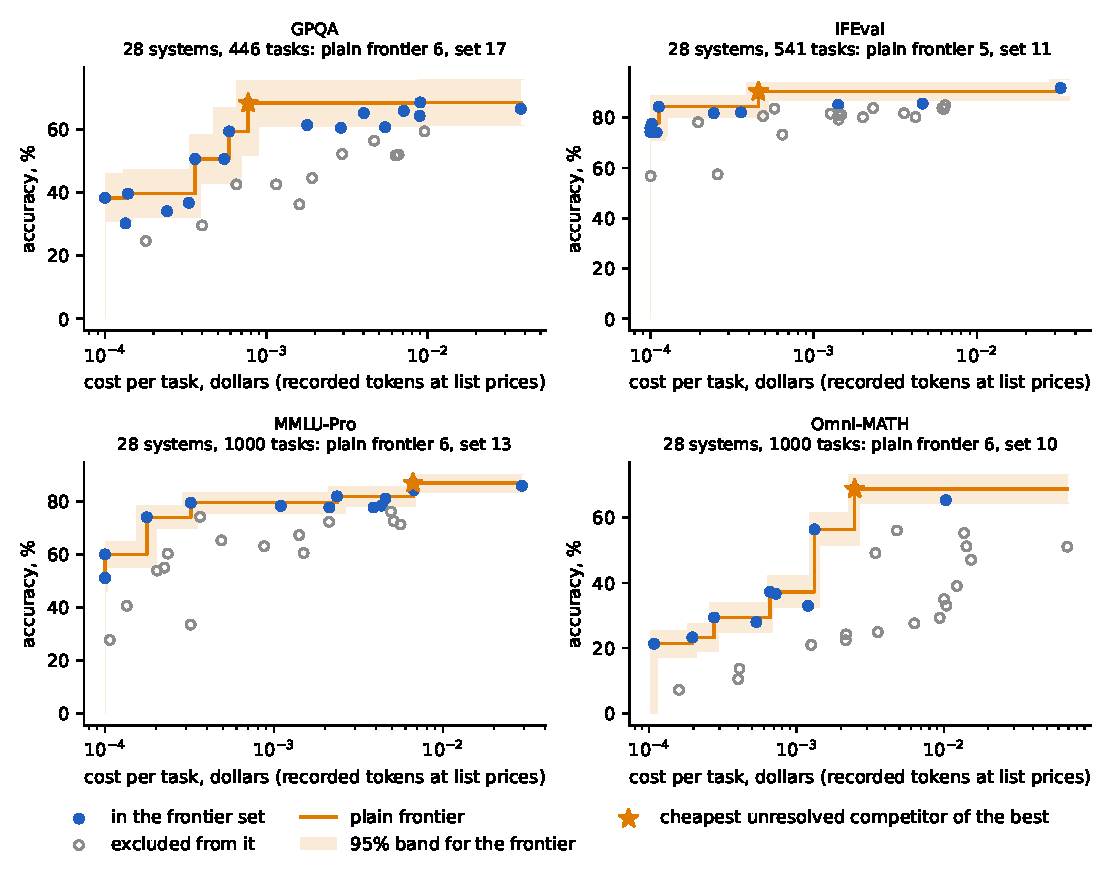
\includegraphics[width=\textwidth]{../figures/figS_helm_frontiers.pdf}
\caption{Cost per task against accuracy on the four HELM Capabilities boards. The orange staircase is the observed frontier. Filled points are systems that cannot be excluded from the frontier at the 5\% level. The star is the cheapest unresolved competitor of the best. The shaded region is the 95\% simultaneous band. Costs below $10^{-4}$ dollars are drawn at $10^{-4}$.}
\end{figure}

\section*{S14. Fresh-task replication of the certificates, board by board}
{\scriptsize\setlength{\tabcolsep}{1.5pt}\begin{longtable}{llrrrrrrr}
\caption{Fresh-task replication of the entrant certificates, board by board. Cases: entrant-holder pairs tested over the random splits; distinct pairs: how many different entrant-holder pairs they are; leads in points. Groups as in Table 9 of the main text.}\label{tab:supp-replication}\\
\toprule
Leaderboard & Board & Group & Cases & Distinct pairs & Lead on D & Lead on V & Positive & Significant \\
\midrule
\endfirsthead
\toprule
Leaderboard & Board & Group & Cases & Distinct pairs & Lead on D & Lead on V & Positive & Significant \\
\midrule
\endhead
\bottomrule
\endfoot
HAL & ColBench backend programming & certified & 14 & 7 & 9.4 & 5.1 & 0.86 & 0.43 \\
HAL & ColBench backend programming & nominal only & 49 & 8 & 5.9 & 4.6 & 1.00 & 0.59 \\
HAL & ColBench backend programming & neither & 212 & 17 & 2.9 & 3.0 & 0.86 & 0.40 \\
HAL & ColBench frontend design & nominal only & 1 & 1 & 3.0 & -2.3 & 0.00 & 0.00 \\
HAL & ColBench frontend design & neither & 32 & 3 & 0.8 & -0.2 & 0.53 & 0.00 \\
HAL & GAIA & nominal only & 6 & 6 & 16.3 & 4.8 & 0.50 & 0.33 \\
HAL & GAIA & neither & 337 & 56 & 5.2 & 6.2 & 0.79 & 0.21 \\
HAL & Online-Mind2Web & certified & 34 & 1 & 14.9 & 13.1 & 1.00 & 1.00 \\
HAL & Online-Mind2Web & nominal only & 5 & 1 & 11.7 & 16.3 & 1.00 & 1.00 \\
HAL & Online-Mind2Web & neither & 266 & 38 & 3.5 & 2.6 & 0.76 & 0.11 \\
HAL & ScienceAgentBench & nominal only & 3 & 3 & 18.3 & 1.3 & 0.67 & 0.00 \\
HAL & ScienceAgentBench & neither & 173 & 25 & 7.9 & 7.3 & 0.87 & 0.20 \\
HAL & USACO & certified & 48 & 4 & 13.8 & 9.2 & 0.98 & 0.83 \\
HAL & USACO & nominal only & 46 & 5 & 10.6 & 10.0 & 0.96 & 0.76 \\
HAL & USACO & neither & 90 & 6 & 4.4 & 4.8 & 0.83 & 0.43 \\
HELM & GPQA & certified & 88 & 13 & 14.1 & 14.0 & 0.99 & 0.92 \\
HELM & GPQA & nominal only & 52 & 12 & 10.5 & 10.6 & 0.98 & 0.90 \\
HELM & GPQA & neither & 189 & 19 & 4.7 & 6.0 & 0.77 & 0.49 \\
HELM & IFEval & certified & 67 & 7 & 7.2 & 6.2 & 1.00 & 0.87 \\
HELM & IFEval & nominal only & 29 & 6 & 5.8 & 7.1 & 0.97 & 0.97 \\
HELM & IFEval & neither & 58 & 4 & 2.5 & 3.5 & 0.90 & 0.43 \\
HELM & MMLU-Pro & certified & 148 & 10 & 13.5 & 14.0 & 1.00 & 0.97 \\
HELM & MMLU-Pro & nominal only & 93 & 9 & 4.6 & 4.4 & 1.00 & 0.62 \\
HELM & MMLU-Pro & neither & 116 & 8 & 2.9 & 4.0 & 1.00 & 0.85 \\
HELM & Omni-MATH & certified & 203 & 9 & 17.1 & 17.6 & 1.00 & 1.00 \\
HELM & Omni-MATH & nominal only & 3 & 2 & 4.7 & 0.6 & 0.33 & 0.33 \\
HELM & Omni-MATH & neither & 63 & 4 & 2.1 & 1.1 & 0.76 & 0.08 \\
\end{longtable}
}
{\scriptsize\setlength{\tabcolsep}{1.5pt}\begin{longtable}{lp{2.4cm}p{3.5cm}p{3.5cm}rrrr}
\caption{The distinct entrant-holder pairs behind the certified cases of the replication. Splits: the number of random splits in which the pair was certified on the discovery half; positive on V: the share of those splits in which the entrant's lead on the fresh half is positive; leads are means over those splits, in points.}\label{tab:supp-replication-pairs}\\
\toprule
Leaderboard & Board & Entrant & Holder & Splits & Positive on V & Lead on D & Lead on V \\
\midrule
\endfirsthead
\toprule
Leaderboard & Board & Entrant & Holder & Splits & Positive on V & Lead on D & Lead on V \\
\midrule
\endhead
\bottomrule
\endfoot
HAL & ColBench backend programming & Hal Generalist Agent (Sonnet3.7) & Hal Generalist Agent (GPT4.1) & 2 & 1.00 & 10.1 & 5.5 \\
HAL & ColBench backend programming & Hal Generalist Agent (Sonnet3.7) & colbench\_\allowbreak text\_\allowbreak sonnet37 & 1 & 1.00 & 9.2 & 3.4 \\
HAL & ColBench backend programming & colbench\_\allowbreak backend\_\allowbreak programming colb~ & colbench\_\allowbreak text\_\allowbreak gpt41 & 2 & 1.00 & 8.1 & 3.1 \\
HAL & ColBench backend programming & colbench\_\allowbreak backend\_\allowbreak programming colb~ & colbench\_\allowbreak text\_\allowbreak deepseekv3 & 2 & 1.00 & 5.7 & 1.3 \\
HAL & ColBench backend programming & colbench\_\allowbreak backend\_\allowbreak programming colb~ & colbench\_\allowbreak text\_\allowbreak deepseekv3 & 4 & 1.00 & 14.1 & 11.5 \\
HAL & ColBench backend programming & colbench\_\allowbreak text\_\allowbreak gpt41 & colbench\_\allowbreak text\_\allowbreak gemmini2flash & 2 & 0.00 & 6.3 & -0.9 \\
HAL & ColBench backend programming & colbench\_\allowbreak text\_\allowbreak gpt41 & colbench\_\allowbreak text\_\allowbreak o4mini & 1 & 1.00 & 6.0 & 3.4 \\
HAL & Online-Mind2Web & Browser-Use\_\allowbreak test(DeepSeek-V3) & Browser-Use(o4-mini-2025-04-16\_\allowbreak lo~ & 34 & 1.00 & 14.9 & 13.1 \\
HAL & USACO & USACO Episodic + Semantic (gpt-5-~ & USACO Episodic + Semantic (o4-min~ & 11 & 1.00 & 14.5 & 9.0 \\
HAL & USACO & USACO Episodic + Semantic (o4-min~ & usaco\_\allowbreak episodic & 29 & 1.00 & 14.8 & 11.3 \\
HAL & USACO & usaco\_\allowbreak episodic & usaco\_\allowbreak episodic & 7 & 1.00 & 9.5 & 2.2 \\
HAL & USACO & usaco\_\allowbreak episodic & usaco\_\allowbreak episodic & 1 & 0.00 & 10.5 & -0.6 \\
HELM & GPQA & meta\_\allowbreak llama-4-scout-17b-16e-instru~ & amazon\_\allowbreak nova-lite-v1:0 & 19 & 1.00 & 10.6 & 11.4 \\
HELM & GPQA & meta\_\allowbreak llama-4-scout-17b-16e-instru~ & amazon\_\allowbreak nova-micro-v1:0 & 8 & 1.00 & 10.7 & 14.0 \\
HELM & GPQA & meta\_\allowbreak llama-4-scout-17b-16e-instru~ & openai\_\allowbreak gpt-4o-mini-2024-07-18 & 4 & 1.00 & 11.0 & 16.8 \\
HELM & GPQA & meta\_\allowbreak llama-4-scout-17b-16e-instru~ & qwen\_\allowbreak qwen2.5-7b-instruct-turbo & 1 & 1.00 & 16.1 & 17.0 \\
HELM & GPQA & openai\_\allowbreak gpt-4.1-2025-04-14 & anthropic\_\allowbreak claude-3-7-sonnet-20250~ & 2 & 0.50 & 10.5 & -0.2 \\
HELM & GPQA & openai\_\allowbreak gpt-4.1-mini-2025-04-14 & meta\_\allowbreak llama-4-scout-17b-16e-instru~ & 8 & 1.00 & 14.2 & 7.3 \\
HELM & GPQA & openai\_\allowbreak gpt-4.1-nano-2025-04-14 & amazon\_\allowbreak nova-lite-v1:0 & 3 & 1.00 & 14.2 & 7.8 \\
HELM & GPQA & openai\_\allowbreak gpt-4.1-nano-2025-04-14 & amazon\_\allowbreak nova-micro-v1:0 & 1 & 1.00 & 12.6 & 12.1 \\
HELM & GPQA & openai\_\allowbreak gpt-4.1-nano-2025-04-14 & openai\_\allowbreak gpt-4o-mini-2024-07-18 & 1 & 1.00 & 13.0 & 14.8 \\
HELM & GPQA & openai\_\allowbreak gpt-oss-120b & meta\_\allowbreak llama-4-scout-17b-16e-instru~ & 19 & 1.00 & 17.0 & 18.4 \\
HELM & GPQA & openai\_\allowbreak gpt-oss-120b & openai\_\allowbreak gpt-4.1-nano-2025-04-14 & 19 & 1.00 & 16.9 & 18.6 \\
HELM & GPQA & openai\_\allowbreak gpt-oss-20b & meta\_\allowbreak llama-4-scout-17b-16e-instru~ & 1 & 1.00 & 14.8 & 2.7 \\
HELM & GPQA & openai\_\allowbreak gpt-oss-20b & openai\_\allowbreak gpt-4.1-nano-2025-04-14 & 2 & 1.00 & 15.0 & 2.5 \\
HELM & IFEval & meta\_\allowbreak llama-4-scout-17b-16e-instru~ & amazon\_\allowbreak nova-lite-v1:0 & 4 & 1.00 & 4.4 & 3.9 \\
HELM & IFEval & meta\_\allowbreak llama-4-scout-17b-16e-instru~ & openai\_\allowbreak gpt-4o-mini-2024-07-18 & 16 & 1.00 & 4.3 & 2.9 \\
HELM & IFEval & openai\_\allowbreak gpt-4.1-mini-2025-04-14 & meta\_\allowbreak llama-3.1-70b-instruct-turbo & 18 & 1.00 & 8.1 & 8.4 \\
HELM & IFEval & openai\_\allowbreak gpt-4.1-mini-2025-04-14 & meta\_\allowbreak llama-4-scout-17b-16e-instru~ & 14 & 1.00 & 8.5 & 8.7 \\
HELM & IFEval & openai\_\allowbreak gpt-4.1-nano-2025-04-14 & amazon\_\allowbreak nova-lite-v1:0 & 13 & 1.00 & 8.7 & 4.8 \\
HELM & IFEval & openai\_\allowbreak gpt-4.1-nano-2025-04-14 & amazon\_\allowbreak nova-micro-v1:0 & 1 & 1.00 & 7.8 & 8.9 \\
HELM & IFEval & openai\_\allowbreak gpt-4.1-nano-2025-04-14 & meta\_\allowbreak llama-3.1-8b-instruct-turbo & 1 & 1.00 & 9.5 & 10.6 \\
HELM & MMLU-Pro & anthropic\_\allowbreak claude-opus-4-20250514 & openai\_\allowbreak gpt-4.1-2025-04-14 & 17 & 1.00 & 5.7 & 3.9 \\
HELM & MMLU-Pro & anthropic\_\allowbreak claude-sonnet-4-5-20250~ & openai\_\allowbreak gpt-4.1-2025-04-14 & 6 & 1.00 & 6.1 & 5.5 \\
HELM & MMLU-Pro & meta\_\allowbreak llama-4-scout-17b-16e-instru~ & amazon\_\allowbreak nova-lite-v1:0 & 18 & 1.00 & 13.3 & 15.1 \\
HELM & MMLU-Pro & meta\_\allowbreak llama-4-scout-17b-16e-instru~ & openai\_\allowbreak gpt-4o-mini-2024-07-18 & 22 & 1.00 & 13.1 & 14.7 \\
HELM & MMLU-Pro & moonshotai\_\allowbreak kimi-k2-instruct & openai\_\allowbreak gpt-4.1-mini-2025-04-14 & 1 & 1.00 & 5.8 & 1.4 \\
HELM & MMLU-Pro & openai\_\allowbreak gpt-4.1-2025-04-14 & anthropic\_\allowbreak claude-3-7-sonnet-20250~ & 1 & 1.00 & 5.2 & 0.2 \\
HELM & MMLU-Pro & openai\_\allowbreak gpt-4.1-mini-2025-04-14 & meta\_\allowbreak llama-4-scout-17b-16e-instru~ & 3 & 1.00 & 6.5 & 1.7 \\
HELM & MMLU-Pro & openai\_\allowbreak gpt-oss-120b & amazon\_\allowbreak nova-lite-v1:0 & 18 & 1.00 & 18.7 & 20.3 \\
HELM & MMLU-Pro & openai\_\allowbreak gpt-oss-120b & openai\_\allowbreak gpt-4o-mini-2024-07-18 & 22 & 1.00 & 18.7 & 19.7 \\
HELM & MMLU-Pro & openai\_\allowbreak gpt-oss-20b & amazon\_\allowbreak nova-lite-v1:0 & 40 & 1.00 & 13.9 & 14.1 \\
HELM & Omni-MATH & meta\_\allowbreak llama-4-scout-17b-16e-instru~ & openai\_\allowbreak gpt-4o-mini-2024-07-18 & 2 & 1.00 & 9.4 & 9.2 \\
HELM & Omni-MATH & meta\_\allowbreak llama-4-scout-17b-16e-instru~ & qwen\_\allowbreak qwen2.5-7b-instruct-turbo & 38 & 1.00 & 7.9 & 7.9 \\
HELM & Omni-MATH & moonshotai\_\allowbreak kimi-k2-instruct & openai\_\allowbreak gpt-4.1-mini-2025-04-14 & 40 & 1.00 & 16.2 & 16.3 \\
HELM & Omni-MATH & openai\_\allowbreak gpt-4.1-2025-04-14 & meta\_\allowbreak llama-4-scout-17b-16e-instru~ & 3 & 1.00 & 10.3 & 9.3 \\
HELM & Omni-MATH & openai\_\allowbreak gpt-4.1-mini-2025-04-14 & meta\_\allowbreak llama-4-scout-17b-16e-instru~ & 40 & 1.00 & 11.9 & 11.8 \\
HELM & Omni-MATH & openai\_\allowbreak gpt-oss-120b & meta\_\allowbreak llama-4-scout-17b-16e-instru~ & 29 & 1.00 & 31.0 & 32.1 \\
HELM & Omni-MATH & openai\_\allowbreak gpt-oss-120b & openai\_\allowbreak gpt-4.1-nano-2025-04-14 & 11 & 1.00 & 31.3 & 33.1 \\
HELM & Omni-MATH & openai\_\allowbreak gpt-oss-20b & meta\_\allowbreak llama-4-scout-17b-16e-instru~ & 29 & 1.00 & 18.9 & 19.4 \\
HELM & Omni-MATH & openai\_\allowbreak gpt-oss-20b & openai\_\allowbreak gpt-4.1-nano-2025-04-14 & 11 & 1.00 & 18.5 & 21.1 \\
\end{longtable}
}

\section*{S15. Resampling task groups on the real boards}
{\scriptsize\setlength{\tabcolsep}{2pt}\begin{longtable}{lp{2.6cm}rrrrrrr}
\caption{Resampling task groups instead of tasks on the real boards with groups we could name (ScienceAgentBench twice: by source repository and by science domain). Set and best set: number of systems that cannot be excluded from the frontier and from the best, when tasks and when groups are resampled; margin: the bootstrap margin in standard-error units; factor: the ratio of the two margins, which can be read as a common factor on every standard error when the departure from independence is a design effect (Section 6 of the main text). The group labels of ScienceAgentBench are the github\_name and domain columns of its public task dataset.}\label{tab:supp-cluster}\\
\toprule
Board & Groups are & Groups & Tasks & Set (tasks) & Set (groups) & Margin (tasks) & Margin (groups) & Factor \\
\midrule
\endfirsthead
\toprule
Board & Groups are & Groups & Tasks & Set (tasks) & Set (groups) & Margin (tasks) & Margin (groups) & Factor \\
\midrule
\endhead
\bottomrule
\endfoot
SWE-bench Verified mini & repository & 2 & 50 & 26 & 24 & 3.66 & 3.36 & 0.92 \\
USACO & division & 4 & 307 & 5 & 8 & 3.04 & 5.52 & 1.82 \\
ScienceAgentBench & source repository & 30 & 102 & 21 & 21 & 3.46 & 4.11 & 1.19 \\
ScienceAgentBench & science domain & 4 & 102 & 21 & 22 & 3.46 & 4.56 & 1.32 \\
\end{longtable}
}

\end{document}
